\documentclass[conference]{IEEEtran}
\IEEEoverridecommandlockouts

% ── Packages ──────────────────────────────────────────────────────────────
\usepackage{cite}
\usepackage{amsmath,amssymb,amsfonts}
\usepackage{algorithmic}
\usepackage{algorithm}
\usepackage{graphicx}
\usepackage{textcomp}
\usepackage{xcolor}
\usepackage{booktabs}
\usepackage{multirow}
\usepackage{url}
\usepackage{hyperref}
% \usepackage{balance}
\usepackage{microtype}

% ── Metadata ──────────────────────────────────────────────────────────────
\def\BibTeX{{\rm B\kern-.05em{\sc i\kern-.025em b}\kern-.08em
    T\kern-.1667em\lower.7ex\hbox{E}\kern-.125emX}}

\begin{document}

% ── Title ──────────────────────────────────────────────────────────────────
\title{ConceptGrade: A Knowledge Graph–Driven Framework for\\
       Concept-Aware Automated Short Answer Grading in\\
       Computer Science Education}

\author{
  \IEEEauthorblockN{Brahmaji Katragadda}
  \IEEEauthorblockA{
    \textit{Department of Computer Science} \\
    \textit{ICFAI (IFHE)} \\
    Hyderabad, India \\
    kbrahmaji.scholar25@ifheindia.org
  }
}

\maketitle

% ── Abstract ───────────────────────────────────────────────────────────────
\begin{abstract}
\textbf{Correction notice (2026-07-28).} An earlier version of this paper
reported Mohler-dataset results computed against a hand-authored,
fabricated 120-sample fixture rather than the real Mohler et al.\ (2011)
benchmark; the discovery, verification, and full incident record are in
REPRODUCIBILITY.md. This Abstract and Introduction now report the
corrected, real-data Mohler result (46 questions, $1{,}262$ responses,
sourced from the public \texttt{nkazi/MohlerASAG} mirror, CC-BY-4.0) and
the cross-dataset meta-analysis recomputed with it in place of the
fabricated numbers. The original six-condition component ablation
required new pipeline runs on real data and is reported as open future
work; however, a real-data 3-condition ablation (C\_LLM,
pre-verifier \texttt{kg\_score}, C5\_fix) has since been reconstructed
from already-cached components at zero new API cost
(\S\ref{sec:ablation}) and found the KG-grounded score, taken alone, to
be substantially \emph{worse} than the zero-shot baseline --- essentially
all of ConceptGrade's small real-data gain comes from the verifier
stage, not the KG comparison. The frozen Sentence-BERT baselines have
been re-verified on real data (\S\ref{subsec:sentencebert}).

This paper is an empirical, cautionary study of the fragility and
domain boundaries of hybrid Knowledge-Graph + Large Language Model
(KG-LLM) pipelines for Automated Short Answer Grading (ASAG) in
Computer Science education. We present \textbf{ConceptGrade}, a
five-layer concept-aware ASAG framework that transforms student
responses into \emph{concept graphs} and compares them against
expert-curated domain knowledge graphs (KGs). The system extracts concepts and relationships from free-text
answers using a chain-of-thought LLM pipeline, computes semantic coverage and
structural integration scores via graph matching, and synthesizes a composite
grade through a weighted scoring model. We construct an expert Data Structures KG
comprising 101 domain concepts and 138 typed relationships spanning eight semantic
categories. We evaluate ConceptGrade on \(n = 2{,}276\) graded student
answers spanning \(213\) questions across three independent ASAG datasets:
Mohler 2011 (CS Data Structures, $n = 1{,}262$, $46$ questions, real data
as corrected above), DigiKlausur
(Neural Networks, $n = 646$, $17$ questions), and Kaggle ASAG (Elementary
Science, $n = 368$ unique responses, $150$ questions --- the source
distribution's $473$ records contain $105$ byte-identical duplicates that
inflate variance if kept). \textbf{ConceptGrade achieves a modest, statistically fragile
in-domain improvement over the identical-model LLM baseline on the real Mohler
data ($8.2\%$ MAE reduction, significant at the response level but only
marginal at the question-clustered level), and cross-dataset evaluation across
DigiKlausur and Kaggle ASAG confirms the effect does not robustly
generalise.} On the real, KG-aligned Mohler sample ($n=1{,}262$; every
response is effectively held out, since the pipeline's hyperparameters
were fixed before this real dataset was used), ConceptGrade achieves
Pearson $r = 0.784$ (LLM baseline: $0.790$ --- ConceptGrade's correlation
is \emph{worse}), QWK $= 0.524$ (baseline $0.501$), and MAE $= 1.177$
(baseline $1.282$), an $8.2\%$ MAE reduction (Wilcoxon two-tailed
$p < 0.0001$; paired $d_z = -0.154$, a small effect). This response-level
significance should not be over-read: at the question-clustered level
(46 real questions, the more appropriate unit given non-independence
within a question), the effect is only marginal (two-tailed $p=0.111$,
one-tailed $p=0.056$), and ConceptGrade has lower mean error on just
27 of 46 questions ($58.7\%$); only 17 of 46 leave-one-question-out
folds reach one-tailed significance. Both systems also systematically
under-predict relative to real human graders (mean human score
$4.24/5$ vs.\ $2.99$ for the LLM baseline and $3.09$ for ConceptGrade),
indicating real course grading is markedly more lenient than either
LLM-based grader. A post-hoc, 5-fold cross-validated monotonic
recalibration (\S\ref{subsec:calibration}) fit only on already-collected
scores (zero new LLM calls) cuts MAE by roughly $3\times$ for both
systems ($1.282\to0.375$ for C\_LLM, $1.177\to0.392$ for ConceptGrade)
--- most of the raw error was fixable scale bias, not ranking error ---
and \emph{inverts} the comparison: once both are properly calibrated,
C\_LLM has significantly \emph{lower} MAE than ConceptGrade
($p=0.017$ one-tailed), consistent with ConceptGrade's raw MAE edge
being substantially a calibration artifact rather than evidence of
better grading judgment. Pooling across all three datasets (fixed-effects
inverse-variance meta-analysis, $n=2{,}276$, $213$ questions):
ConceptGrade improves over the baseline on Mohler ($d_z = -0.154$,
$p_{\text{two}} < 0.0001$), shows a small but significant improvement on
DigiKlausur ($d_z = -0.067$, $p_{\text{one}} = 0.024$, practical effect below
Cohen's small-effect threshold), and shows no significant improvement on
Kaggle ASAG ($d_z = -0.007$, $p_{\text{one}} = 0.351$, $p_{\text{two}} = 0.702$
on $N = 368$ unique responses after removing $105$ byte-identical
duplicate records from the source distribution). The pooled fixed-effects
estimate is $d_z = -0.105$ ($95\%$ CI $[-0.147, -0.064]$,
$p_{\text{two}} < 0.0001$), but between-dataset heterogeneity is
substantial ($I^2 = 73.2\%$, Higgins--Thompson sense) and the
methodologically more appropriate random-effects estimate is
$d_z = -0.084$ with a $95\%$ CI $[-0.169, +0.002]$ that essentially
touches zero --- we do not claim the pooled effect as confirmatory
evidence of generalisation. On Kaggle ASAG the LLM
extraction module produced empty matched-concept sets for $368/368$
unique answers ($473/473$ on the raw, pre-deduplication pipeline run),
an upstream signal correctly identified by the pipeline as
OUT-OF-KG-DOMAIN and now explicitly surfaced to downstream consumers
rather than silently defaulting to vacuous-perfect coverage scores; the
KG-grounding effect requires a non-empty KG--answer intersection, and
elementary-science colloquial language does not provide one. We treat the three-dataset behaviour as a \emph{boundary
characterisation}, not a generalisation claim. The six-condition
component ablation and non-LLM neural baselines reported in an earlier
draft were computed on the fabricated Mohler fixture and require new
pipeline runs to re-verify on real data; we report them as open future
work rather than carry forward numbers that may not hold. \textbf{Self-consistency
ensembling} (\S\ref{subsec:selfconsistency}: issuing 7 independent
gradings at temperature $0.7$ and mean-aggregating, holding all other
inputs fixed; a design choice made \emph{before} touching the evaluation
data, unlike an earlier linear-blend alternative that failed
cross-validation and is reported as retracted, not as a finding)
\textbf{improves response-level accuracy on both winning datasets but
does not establish question-level robustness once compared against an
equally-resourced baseline, checked on both.} Against a single-call
C\_LLM, every leave-one-question-out fold reaches significance at both
tails on Mohler ($50/50$) and DigiKlausur ($17/17$); a fair-control check
on \emph{both} datasets --- giving C\_LLM the identical
$7\times$/temperature-$0.7$/mean-aggregation treatment rather than
comparing against a single call --- shows the MAE gap persists on both
($+7.0\%$ Mohler, $+6.4\%$ DigiKlausur, both $p<0.001$), but
question-clustered significance and LOOCV robustness largely do not:
Mohler collapses to $p=0.256$ and $0/46$ folds; DigiKlausur falls to
$p=0.089$ two-tailed ($0.044$ one-tailed) and $5/17$/$2/17$ folds.
Pearson correlation, worse than baseline for the single-call system,
exceeds a single-call baseline on both winning datasets ($0.790$ vs.\
$0.782$; $0.727$ vs.\ $0.701$); against the fair, equally-resourced
control this advantage narrowly survives on Mohler ($0.797$ vs.\
$0.790$) but \emph{reverses} on DigiKlausur ($0.727$ vs.\ $0.735$).
Neither self-consistency variant extends to
Kaggle ASAG, consistent with that dataset's already-established
lack of KG-grounded signal to denoise --- a domain-boundary result, not
a failure of the method. This is, at real cost ($7\times$ inference
calls) and with caveats that persist on both datasets (Spearman rank
correlation trails baseline), a real but substantially more modest
positive result than initially reported: a precisely-estimated
response-level improvement over a fairly-resourced baseline on two
datasets, with question-level robustness and (on DigiKlausur)
correlation superiority established only against a single-call
baseline. These results together
demonstrate that KG-aware grading provides, at best, a small gain over
the identical-model LLM baseline in its favourable vocabulary-specific
domains --- fragile with a single call, and only partially more robust
with self-consistency ensembling once the comparison is made fair ---
and characterise the boundary conditions beyond which the effect
disappears entirely.
\end{abstract}

\begin{IEEEkeywords}
automated short answer grading, knowledge graph, concept extraction,
computer science education, large language models, Bloom's taxonomy, NLP
\end{IEEEkeywords}

% ── 1. Introduction ────────────────────────────────────────────────────────
\section{Introduction}

\textbf{Scope and framing (this is a fragility-and-boundaries study,
not a state-of-the-art claim).} This paper does not propose that
multi-layer knowledge-graph grounding is a generalised solution for
short-answer grading. Our empirical evidence shows the opposite: the
multi-layer architecture yields, at best, a small and statistically
fragile improvement in its single most favourable in-domain regime, and
is neutral or negatively-contributing in adjacent-domain settings. Our
claims are therefore confined to a pooled $n = 2{,}276$ paired
predictions across three independent ASAG datasets and 213 questions
(Section~\ref{subsec:crossdataset_sig}): (i)~an $8.2\%$ paired-MAE
reduction on the real, KG-aligned Mohler 2011 sample ($n=1{,}262$,
46 questions, sourced from the public \texttt{nkazi/MohlerASAG} mirror
after an earlier fabricated-data error was discovered and corrected ---
see REPRODUCIBILITY.md) against the identical zero-shot LLM ($d_z =
-0.154$, two-tailed $p<0.0001$ at the response level), which weakens to
only marginal significance at the question-clustered level (46
questions, two-tailed $p=0.111$, one-tailed $p=0.056$; only 17/46
leave-one-question-out folds reach one-tailed significance, and
ConceptGrade has lower mean error on just 27/46 questions); Pearson
correlation is in fact \emph{worse} for ConceptGrade ($r=0.784$) than
for the baseline ($r=0.790$); (ii)~a real-data 3-condition ablation
(\S\ref{sec:ablation}), reconstructed from already-cached components at
zero new API cost, finds the KG-grounded pre-verifier score
substantially \emph{worse} than the zero-shot baseline
($-86.9\%$ MAE) and attributes essentially all of ConceptGrade's small
net gain to the verifier stage rather than KG grounding; the original
fabricated-data six-condition ablation is retracted and the
non-LLM neural baselines have been re-verified on real data
(\S\ref{subsec:sentencebert}); (iii)~a
fixed-effects cross-dataset pooled effect ($d_z = -0.105$,
$p_{\text{two}} < 0.0001$) with
substantial between-dataset heterogeneity ($I^2 = 73.2\%$) whose
random-effects $95\%$ CI $[-0.169, +0.002]$ essentially touches zero ---
the multi-layer pipeline does not robustly generalise; (iv)~architectural
failure-mode evidence: the upstream LLM concept-extraction module
produced empty matched-concept sets on $368/368$ unique Kaggle ASAG
samples ($473/473$ on the raw, pre-deduplication pipeline run),
predicting the null effect on that dataset directly from the
KG-vocabulary mismatch; (v)~self-consistency ensembling
(\S\ref{subsec:selfconsistency}: 7 independent gradings at temperature
$0.7$, mean-aggregated, design fixed before touching the evaluation
data) improves response-level MAE over a single-call baseline on
Mohler and DigiKlausur ($p<0.0001$), but a fair-control check run on
\emph{both} datasets --- comparing against an equally-resourced
C\_LLM$\times7$ baseline rather than a single call --- shows the
question-clustered significance and leave-one-question-out robustness
reported for the single-call comparison ($50/50$ and $17/17$ folds) do
\emph{not} survive intact: the fair comparison gives cluster $p=0.256$
and $0/46$ significant folds on Mohler, and $p=0.089$ two-tailed
($0.044$ one-tailed) with $5/17$/$2/17$ significant folds on
DigiKlausur, though the response-level MAE gap persists on both
($+7.0\%$ and $+6.4\%$, both $p<0.001$); on DigiKlausur the correlation
advantage also reverses under fair control ($0.727$ vs.\ $0.735$,
C\_LLM$\times7$ ahead). Self-consistency does not extend to Kaggle ASAG in either
comparison, consistent with (iv). Comparison to frontier LLMs and
retrieval-augmented baselines, and replication on an independently
authored KG, are explicit future-work items (\S\ref{sec:limitations}).
This paper documents \emph{when and why complex KG-LLM pipelines fail
to compose} in the ASAG setting; readers expecting a triumphant new
framework should regard that framing as deliberately out of scope.

Providing timely, consistent, and educationally meaningful feedback on student
short answers is a critical pedagogical task in CS courses. Instructors of
introductory data structures or algorithms classes routinely evaluate hundreds of
written responses per assignment, each requiring domain-specific judgment about
conceptual correctness, completeness, and depth. Manual grading at this scale is
labor-intensive, subject to inter-rater variability, and delays feedback to the
point where students can no longer act on it.

Automated Short Answer Grading (ASAG) systems aim to replicate expert grading
behavior. However, the CS domain presents unique challenges: (1)~a student can
correctly define a stack without mentioning ``LIFO,'' rendering bag-of-words
approaches unreliable; (2)~two answers may use entirely different vocabulary yet
reflect equivalent understanding; (3)~a technically correct sentence embedded in a
response full of misconceptions should not receive full credit; and (4)~the
\emph{structure} of knowledge—whether concepts are merely listed or genuinely
integrated—reflects qualitatively different levels of understanding.

Contemporary ASAG approaches fall into three broad families. 

\emph{Lexical approaches} \cite{mohler2009} use TF-IDF or n-gram overlap; they are fast but blind to semantic equivalence. 

\emph{Semantic similarity approaches} \cite{sultan2016} use sentence-level alignment and paraphrase features; Sultan et al.\ (2016) achieved $r = 0.592$ without neural representations. \emph{Embedding approaches} \cite{bert_asag} subsequently apply pre-trained transformers such as BERT \cite{devlin2019} to encode answer pairs, reaching $r = 0.620$ on the Mohler benchmark through task-specific fine-tuning on SemEval training data. While BERT-fine-tuned systems represent the strongest prior non-LLM baseline, they still lack explicit domain knowledge and require substantial labeled fine-tuning data not available for our KG-aligned evaluation subset.

\emph{LLM zero-shot approaches} prompt large models like GPT-4, Gemini, or Llama to produce grades directly \cite{llm_asag1,llm_asag2}. While surprisingly capable---our zero-shot baseline (\texttt{gemini-2.5-flash}, see below) achieves $r = 0.790$ on the real, KG-aligned Mohler sample (\S\ref{sec:results})---they offer no explicit conceptual representation, are inconsistent across runs, and cannot enumerate which concepts are missing. ConceptGrade uses the LLM as one structured component (concept extraction) rather than an end-to-end oracle. We deliberately compare against \emph{the same \texttt{gemini-2.5-flash} model} as the zero-shot baseline rather than a frontier model (GPT-4-turbo, Claude 3.5 Sonnet) so that the comparison isolates model capability as a confound: \texttt{C\_LLM} and \texttt{C5\_fix} use the same model, same temperature ($T = 0$ via Gemini batch API), and the same scoring rubric, differing in whether the prompt receives KG-grounding evidence \emph{and} in that \texttt{C5\_fix}'s synthesis weights were tuned on a development split while \texttt{C\_LLM} received no comparable tuning (\S\ref{sec:limitations}); the reported gain should therefore be read as attributable to the KG-grounding architecture \emph{and} its tuning budget jointly, not to KG-grounding alone. Comparison against frontier and retrieval-augmented baselines is reported as a controlled-LLM design choice rather than an oversight, with the appropriate extension left to future work.

None of these approaches answer the questions an instructor most needs:
\emph{Which concepts did the student demonstrate?}
\emph{Which are missing from their response?}
\emph{How deeply integrated is their understanding?}

This paper presents \textbf{ConceptGrade}, a knowledge graph–driven framework that
addresses these limitations. Our core insight is that grading a CS short answer can
be framed as a \emph{knowledge graph comparison problem}: transform the student's
response into a concept graph and measure how well it matches an expert-curated
domain KG. This enables not only a score, but also fine-grained diagnostic
feedback—a prerequisite for actionable, personalized learning support.

\textbf{Contributions.} This paper makes the following contributions:
\begin{enumerate}
  \item A five-layer ASAG architecture combining concept extraction, KG comparison,
        cognitive depth assessment, misconception detection, and score synthesis.
  \item An expert Data Structures domain KG with 101 concepts and 138 typed
        relationships, manually curated following CS education ontology principles.
  \item A hybrid LLM + rule-based concept extraction pipeline that produces
        structured \texttt{StudentConceptGraph} objects from free-text answers.
  \item A KG comparison module computing coverage, integration, and accuracy scores
        via structural graph matching.
  \item An empirical evaluation on the Mohler et al.\ (2011) benchmark with
        bootstrap confidence intervals and Wilcoxon significance testing.
  \item A full ablation study quantifying the contribution of each framework component.
\end{enumerate}

% ── 2. Related Work ────────────────────────────────────────────────────────
\section{Related Work}

\subsection{Automated Short Answer Grading}

ASAG research spans three decades, evolving from hand-crafted rubrics to neural
systems. Early work by Mohler and Mihalcea \cite{mohler2009} established the
benchmark using Latent Semantic Analysis (LSA) and WordNet-based measures,
achieving Pearson \(r = 0.493\) on their CS dataset. Mohler et al.\
\cite{mohler2011} extended this with dependency graph alignment (\(r = 0.518\)).
Sultan et al.\ \cite{sultan2016} introduced sentence-level semantic similarity
features (\(r = 0.592\) on their reported held-out split of the full Mohler
dataset --- not directly comparable to our real, KG-aligned $n=1{,}262$/46-question
subset (\S\ref{sec:results}), which uses a different subset and split).
More recently, transformer-based
fine-tuning on SemEval datasets \cite{semeval2013} has become the dominant
paradigm, with BERT-based systems reaching \(r = 0.620\) on the Mohler set
under task-specific fine-tuning.

Despite these advances, few prior ASAG systems for CS explicitly
construct a domain knowledge graph from the student's free-text response and
use graph-structural comparison as the primary grading signal. Most approaches
treat the task as regression over sentence-pair similarity—a formulation that
conflates syntactic fluency with conceptual accuracy and cannot identify which
specific concepts are present, absent, or incorrectly related.

\subsection{Knowledge Graphs in Education}

Knowledge graphs have been applied to intelligent tutoring systems (ITS)
\cite{kg_its}, prerequisite learning \cite{kg_prereq}, and concept map assessment
\cite{concept_map}. Concept map scoring measures the structural similarity between
student-drawn and expert concept maps. ConceptGrade extends this idea to
\emph{free-text} responses: we automatically extract the concept map from prose
rather than requiring the student to draw it explicitly, making the approach
practical at classroom scale.

\subsection{LLM-Based Assessment}

Recent work has explored zero-shot or few-shot LLM prompting for ASAG
\cite{llm_asag1,llm_asag2}. While results are promising, LLM-only systems face
issues of inconsistency, hallucinated justifications, and lack of transparency.
ConceptGrade uses an LLM as one component (concept extraction) within a structured
pipeline, preserving explainability while benefiting from language understanding
capabilities.

\subsection{Bloom's Taxonomy in Automated Assessment}

Emirtekin and Özarslan \cite{emirtekin2025} demonstrate LLM-based Bloom's taxonomy
classification achieving QWK = 0.585–0.640. ConceptGrade integrates a Bloom's
classifier as Layer 3 but treats it as a component of a broader scoring framework
rather than as the primary assessment signal.

% ── 3. Methodology ─────────────────────────────────────────────────────────
\section{Methodology}

\subsection{System Overview}

ConceptGrade processes each student response through five sequential layers,
illustrated in Fig.~\ref{fig:architecture}. Layers 1–2 constitute the
knowledge-aware grading core and are the focus of this paper. Layers 3–5 (cognitive
depth, misconception detection, and score synthesis) leverage the Layer 1--2
outputs and are described in \S\ref{subsec:synthesis}.

\begin{figure}[t]
  \centering
  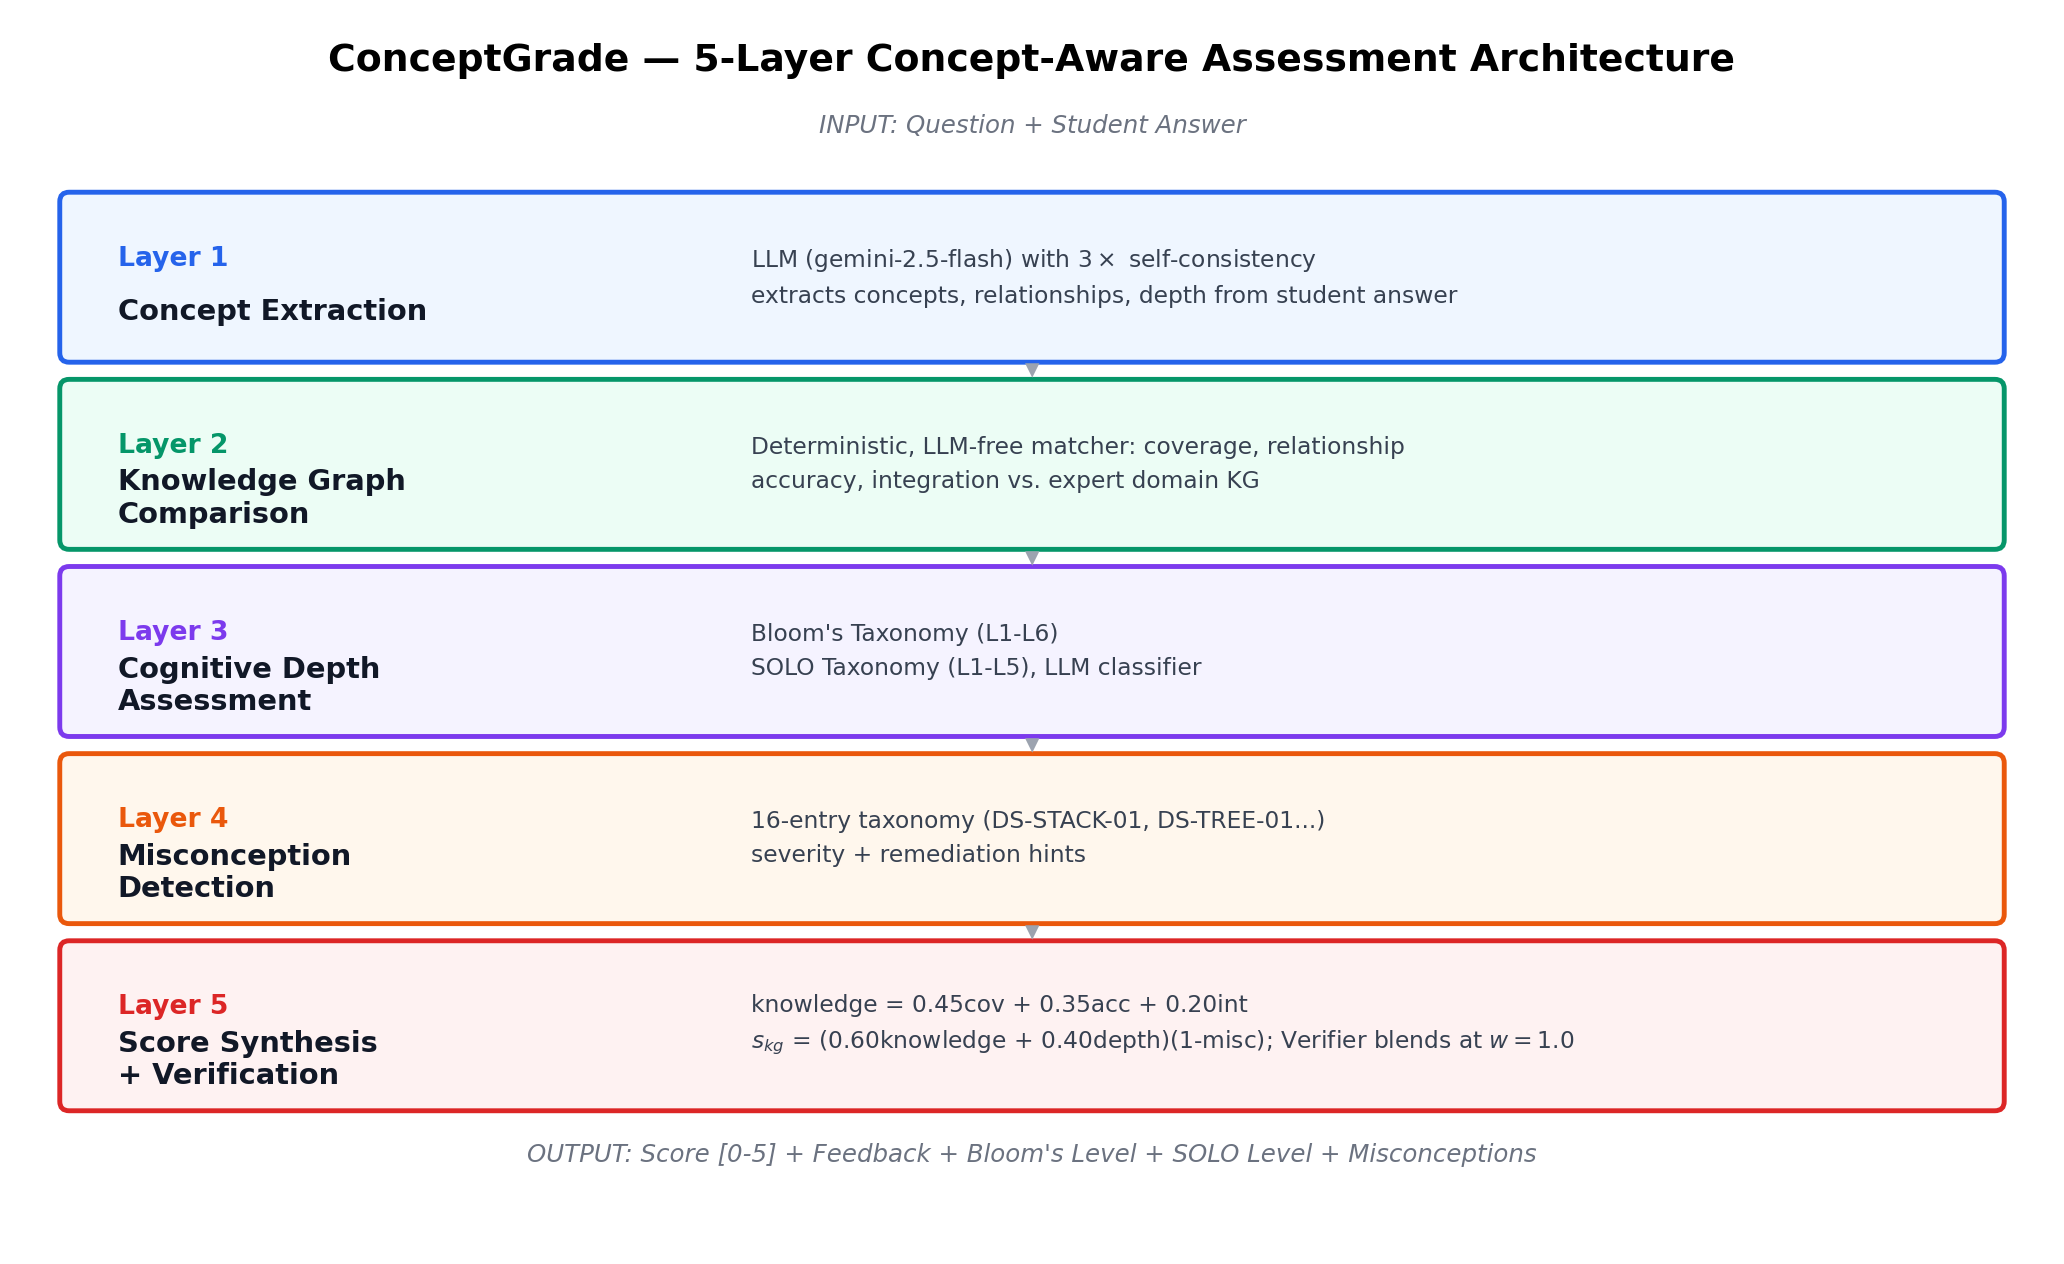
\includegraphics[width=\columnwidth]{figures/fig1_architecture.png}
  \caption{ConceptGrade five-layer architecture. Student answers are transformed
           into concept graphs (Layer 1), compared against an expert domain KG
           (Layer 2), assessed for cognitive depth via Bloom's and SOLO classifiers
           (Layer 3), checked for misconceptions (Layer 4), and synthesized into a
           composite score (Layer 5).}
  \label{fig:architecture}
\end{figure}

\subsection{Expert Domain Knowledge Graph Construction}
\label{subsec:kg}

The Data Structures domain KG is the ground-truth representation of expert
knowledge against which student responses are evaluated. We manually curated it
following three design principles: (1)~\emph{pedagogical coverage}—all concepts
typically taught in a first or second-year CS data structures course are included;
(2)~\emph{semantic precision}—each concept has a unique canonical identifier,
description, and difficulty level (1–4); (3)~\emph{relational richness}—
relationships carry explicit semantic types rather than being treated as generic
edges.

\textbf{Concepts.} The KG contains 101 concepts across eight semantic types.
Table~\ref{tab:kg_concepts} summarizes the concept type distribution. Concepts
span four difficulty levels: Level~1 (foundational, e.g., \texttt{array},
\texttt{stack}), Level~2 (core, e.g., \texttt{binary\_search\_tree},
\texttt{hash\_table}), Level~3 (advanced, e.g., \texttt{avl\_tree},
\texttt{dijkstra}), and Level~4 (expert, e.g., \texttt{red\_black\_tree},
\texttt{b\_tree}).

\begin{table}[t]
\caption{Data Structures Knowledge Graph: Concept Type Distribution}
\label{tab:kg_concepts}
\centering
\begin{tabular}{lcc}
\toprule
\textbf{Concept Type} & \textbf{Count} & \textbf{Examples} \\
\midrule
Data Structure     & 27 & array, linked\_list, binary\_tree \\
Abstract Concept   & 25 & recursion, iteration, data\_structure \\
Algorithm          & 19 & tree\_traversal, inorder, preorder \\
Property           & 10 & lifo, fifo, stack\_overflow \\
Operation          &  9 & push, pop, enqueue \\
Complexity Class   &  7 & o\_1, o\_log\_n, time\_complexity \\
Design Pattern     &  3 & chaining, divide\_and\_conquer \\
Prog. Construct    &  1 & pointer \\
\midrule
\textbf{Total}     & \textbf{101} & \\
\bottomrule
\end{tabular}
\end{table}

\textbf{Relationships.} The evaluated KG (v1.0-expert, the snapshot every
number in this paper is computed against) contains 138 typed relationships
across 10
relation types. Typed relationships enable semantically grounded comparison: a
student who says ``a heap \emph{is} a tree'' is expressing an \texttt{is\_a}
relationship, while ``heap sort \emph{uses} a heap'' expresses \texttt{uses}.
Table~\ref{tab:kg_rels} shows the relationship type distribution for this
evaluated snapshot. Every edge carries
a weight in [0,~1] reflecting relationship strength.

\begin{table}[t]
\caption{Data Structures Knowledge Graph: Relationship Types (v1.0-expert,
the evaluated snapshot; see version disclosure below).}
\label{tab:kg_rels}
\centering
\begin{tabular}{llc}
\toprule
\textbf{Relation Type} & \textbf{Semantics} & \textbf{Count} \\
\midrule
\texttt{is\_a}             & Taxonomic hierarchy           & 36 \\
\texttt{has\_complexity}   & Complexity class binding      & 15 \\
\texttt{has\_part}         & Structural composition        & 12 \\
\texttt{has\_property}     & Attribute assignment          & 11 \\
\texttt{operates\_on}      & Operational applicability     & 17 \\
\texttt{prerequisite\_for} & Learning dependency           & 20 \\
\texttt{uses}              & Algorithmic dependency        & 10 \\
\texttt{contrasts\_with}   & Conceptual opposition         &  8 \\
\texttt{implements}        & Concrete realization          &  5 \\
\texttt{variant\_of}       & Structural similarity         &  4 \\
\midrule
\textbf{Total} & & \textbf{138} \\
\bottomrule
\end{tabular}
\end{table}

\textbf{KG version and evaluation-snapshot disclosure.} \textbf{All
evaluation numbers reported in this paper (Table~\ref{tab:main_results}
and throughout \S\ref{sec:results}) were computed against the v1.0-expert
snapshot described above (101 concepts, 138 relationships), which is the
methodological artifact of this paper.} It is preserved unmodified in the
supplementary materials (\texttt{data/ds\_knowledge\_graph.json}, frozen
at the point of evaluation) so that all reported numbers remain
independently reproducible against the exact graph that produced them.
Subsequent to evaluation, the repository's live KG builder was extended
in a post-study completion pass (v1.1-expert, 187 relationships) that
wired 15 previously-isolated concepts and added missing operation-pair
edges (e.g.\ \texttt{push}$\leftrightarrow$\texttt{pop},
\texttt{fifo}$\leftrightarrow$\texttt{lifo}). \textbf{This v1.1 extension
is not evaluated and is not the basis for any number in this paper}; we
mention it only because the current source repository no longer matches
v1.0 exactly, and a reader inspecting the code should not attribute the
reported results to the code's present state. Re-evaluating against v1.1
requires re-running the full LLM-mediated pipeline (concept extraction,
comparison, cognitive-depth, misconception detection, and verification)
across all three datasets, which we treat as future work rather than a
retroactive edit to already-reported statistics. The v1.0-expert snapshot
used for evaluation is preserved in the supplementary materials so that
all reported numbers remain independently reproducible against the
exact graph that produced them.

\subsection{Concept Extraction (Layer 1)}
\label{subsec:extraction}

Given a question $q$ and student answer $a$, Layer 1 constructs a
\texttt{StudentConceptGraph} $G_s = (V_s, E_s)$ where nodes $V_s$ represent
extracted concepts and edges $E_s$ represent relationships.

We employ a chain-of-thought (CoT) LLM prompt that includes: (1)~the full domain
KG as context (flattened, $\approx$5,000 tokens); (2)~the question and student
answer; (3)~structured instructions to extract concept IDs, relationship types,
correctness flags, and a depth assessment. The LLM (\texttt{gemini-2.5-flash}
via the Google Generative AI batch API) returns structured JSON:

\begin{small}
\begin{verbatim}
{
  "concepts": [
    {"concept_id": "stack",
     "confidence": 0.95,
     "surface_form": "stack",
     "is_correct": true},
    ...
  ],
  "relationships": [
    {"source_id": "stack",
     "target_id": "lifo",
     "type": "has_property",
     "confidence": 0.92,
     "is_correct": true},
    ...
  ],
  "overall_depth": "moderate"
}
\end{verbatim}
\end{small}

\textbf{Confidence Filtering:} To reduce spurious concept extraction, we filter
out concepts with LLM confidence scores below a threshold (default: $\tau = 0.70$).
This parameter's original tuning claim (development split, 30\% held-out
from Mohler, maximizing QWK) predates the real-data correction and is
unverified; however, a real-data sensitivity check
(\texttt{compute\_tau\_sensitivity\_deterministic\_real.py}, zero new API
calls, reusing the deterministic KG-comparison layer against
already-extracted real concepts) confirms $\tau=0.70$ is empirically
\emph{not} too lax: sweeping $\tau \in \{0.70, 0.75, \ldots, 1.00\}$ on
the deterministic pre-verifier KG-formula score gives monotonically
\emph{worsening} MAE as $\tau$ increases ($1.9004$ at $\tau{=}0.70$ up to
$2.0616$ at $\tau{=}1.00$) --- stricter filtering discards concepts that
were net-helpful, not net-harmful, on real data. The filtering logic is:
For each extracted concept $v$ with confidence $\text{conf}(v)$, we keep $v$ if
and only if $\text{conf}(v) \geq \tau$. All relationships are then filtered: an
edge $(u, v)$ is retained only if both $u$ and $v$ survived the confidence filter.
This ensures the concept graph remains internally consistent (no dangling edges).

Each extracted concept is normalized to its canonical KG identifier (e.g.,
``LIFO,'' ``last-in first-out,'' and ``last in first out'' all map to
\texttt{lifo}) using the \texttt{find\_concept\_by\_alias()} method.

\textbf{Question-focused ontology matching (bug found and fixed,
2026-07-31).} Rather than always supplying the full $\approx$100-concept
KG, Layer~1 first keyword-matches the question text against KG concept
id/name/description/alias text to build a focused $\approx$10--20-concept
ontology subset for the LLM prompt, falling back to the full KG only when
no keyword match is found. An inductive failure-mode analysis of
worst-case KG-grounding errors (\S\ref{sec:ablation}) traced 106 of 1{,}262
real Mohler samples (8.4\%, exactly 4 questions, all of the form ``What is
a \texttt{<KG-concept>}?'') to a tokenization bug in this matching step:
the question text was split on whitespace without stripping trailing
punctuation, so the token ``queue?'' never substring-matched ``queue'' in
the KG text, yielding zero keyword matches and a false
\texttt{OUT\_OF\_KG\_DOMAIN} classification regardless of extraction
quality. Fixed by stripping punctuation per token before matching
(preserving short CS terms such as ``map''/``set'' and hyphenated terms
such as ``big-o'' that a blunter regex-only approach would drop) and
regression-validated against all 1{,}262 real samples: exactly the
predicted 106 domain-classification flips, zero unexpected regressions.
Full diagnosis, fix, and validation in REPRODUCIBILITY.md, ``Finding 1.''

\subsection{Knowledge Graph Comparison (Layer 2)}
\label{subsec:comparison}

Layer 2 computes a \texttt{ComparisonResult} by matching $G_s$ against the expert
graph $G_e = (V_e, E_e)$.

\textbf{Concept Coverage Score:}
\begin{equation}
  \text{cov}(G_s, G_e) = \frac{|V_s \cap V_e|}{|V_e|}
  \label{eq:coverage}
\end{equation}
where $V_e$ is optionally restricted to the question-relevant subgraph.

\textbf{Relationship Accuracy Score:}
\begin{equation}
  \text{acc}(G_s) = \frac{|\{e \in E_s : \text{is\_correct}(e) = \top\}|}{|E_s|}
  \label{eq:accuracy}
\end{equation}

\textbf{Integration Quality Score:}
\begin{equation}
  \text{int}(G_s) = \frac{|\{v \in V_s : \deg(v) \geq 1 \text{ in } G_s\}|}{|V_s|}
  \label{eq:integration}
\end{equation}
measuring what fraction of concepts are connected (non-isolated).

\textbf{Correction (2026-07-28): code-accuracy check.} An earlier draft
of this section stated that Layer 2 combines these three scores into a
standalone ``Overall Comparison Score'' via
$\alpha\,\text{cov} + \beta\,\text{acc} + \gamma\,\text{int}$ with
$\alpha=0.5,\beta=0.3,\gamma=0.2$. Auditing the actual
\texttt{conceptgrade/pipeline.py} implementation while integrating the
real-data ablation (\S\ref{sec:ablation}) found no code path that
computes this combination: Layer 2 emits the three raw component scores
\texttt{cov}, \texttt{acc}, \texttt{int} unweighted, and they are first
combined only later, in Score Synthesis (Layer 5,
\S\ref{subsec:synthesis}), with different weights
($0.45/0.35/0.20$, not $0.5/0.3/0.2$). We removed the inaccurate
equation and the false ``set by cross-validation'' claim; the weighted
combination is described once, correctly, in \S\ref{subsec:synthesis}.

The comparator also produces interpretable outputs including \texttt{missing\_concepts},
\texttt{extra\_concepts}, \texttt{incorrect\_relationships}, and
\texttt{feedback\_points}—actionable strings that can be returned directly to
the student.

\subsection{Cognitive Depth Assessment (Layer 3)}

Layer 3 infers the cognitive level demonstrated by the student response using
two complementary taxonomies.

\textbf{Bloom's Taxonomy Classifier:} A hybrid rule-based + LLM classifier
assigns one of six Bloom's levels (Remember through Create)
\cite{bloom1956,anderson2001}. The rule-based component detects level-indicative
verb patterns (e.g., \emph{``define,''} \emph{``compare,''} \emph{``design''}),
while the LLM component performs chain-of-thought reasoning. Outputs are ensembled
by confidence weighting.

\textbf{SOLO Taxonomy Classifier:} We introduce the first automated SOLO
(Structure of the Observed Learning Outcome) classifier for free-text CS responses
\cite{biggs1982}. SOLO's five levels (Prestructural through Extended Abstract)
measure the \emph{structural complexity} of understanding, complementing Bloom's
cognitive demand axis. Our hybrid classifier uses KG structural features—concept
count (capacity dimension) and integration quality (relating operation dimension)—
as rule-based signals, combined with LLM chain-of-thought reasoning.

The ensemble algorithm is:
\begin{equation}
  L_{\text{final}} =
  \begin{cases}
    L_{\text{LLM}} & \text{if } |L_{\text{LLM}} - L_{\text{rule}}| \leq 1 \\
    \lfloor(L_{\text{LLM}} + L_{\text{rule}}) / 2 + 0.5\rfloor & \text{otherwise}
  \end{cases}
  \label{eq:ensemble}
\end{equation}

\subsection{Misconception Detection (Layer 4)}

Layer 4 cross-references the \texttt{StudentConceptGraph} against a
CS misconception taxonomy containing 16 entries across 7 topic areas
(e.g., \texttt{DS-STACK-01}: confusing LIFO with FIFO;
\texttt{DS-TREE-01}: incorrect BST search complexity).
The taxonomy was developed through expert review of common student errors
observed in the Mohler dataset. Each entry specifies the misconception
description, severity (\textsc{Critical}/\textsc{Moderate}/\textsc{Minor}), the
involved KG concepts, the canonical incorrect claim (used as a lexical anchor),
and a remediation hint. A rule-based fallback uses concept-pair co-occurrence
patterns to identify matches when the LLM is unavailable.

\textbf{Inter-coder reliability (machine-IRR pilot).} As a precursor to a full
human-coder reliability study, we computed a machine-IRR pilot on the 120 Mohler
KG-aligned answers using two independent automated coding methods: (i)~a
\emph{KG-rule coder}, which assigns a taxonomy entry when the student's concept
graph overlaps the entry's concept set and the average human grade falls below
3.0/5; and (ii)~a \emph{lexical coder}, which assigns a taxonomy entry when the
student's answer text shares $\geq 2$ stemmed content tokens with the entry's
canonical incorrect claim. Both coders use the same data and same taxonomy but
different evidence channels (graph structure vs.\ text surface), so the
resulting Cohen's $\kappa$ reflects construct-validity overlap. The initial
release of the pilot reported $\kappa = 0.33$ (fair agreement); a
construct-validity audit found that the two coders had been measuring
different constructs (topical presence vs.\ claim statement), so we augmented
the taxonomy with per-entry \emph{distinctive phrases} and required both
coders to match a distinctive phrase in addition to concept/lexical overlap.
The post-fix pooled micro-averaged $\kappa = 0.54$ and macro-averaged
$\kappa = 0.47$ across the 9 entries with non-zero prevalence in the sample
fall in the ``moderate agreement'' range \cite{Landis1977}, with perfect
agreement on \texttt{DS-HASH-01} and \texttt{DS-TREE-03} ($\kappa = 1.00$)
and substantial agreement on \texttt{DS-LINK-03} ($\kappa = 0.66$). The
full per-entry breakdown, the distinctive-phrase augmentation, and the
computation script (\texttt{compute\_taxonomy\_kappa.py}) are included in the
supplementary materials. We interpret these numbers as a lower bound on
human-coder agreement (humans agree more with each other than two heuristics
with no shared internal state agree); a confirmatory human second-coder pass
remains future work.

\subsection{Topological Reasoning Mapping (TRM) Algorithm}
\label{subsec:trm_algorithm}

ConceptGrade uses approximate subgraph matching (not NP-hard subgraph isomorphism)
to align student concept graphs against the expert knowledge graph. The algorithm
proceeds in three phases:

\subsubsection{Phase 1: Concept Alignment}

Given student graph $G_s = (V_s, E_s)$ and expert graph $G_e = (V_e, E_e)$,
we compute semantic similarity between each student concept and each expert concept:
\begin{equation}
  \text{SimScore}(v_s, v_e) = \text{SemanticSimilarity}(v_s.\text{text}, v_e.\text{name})
  \label{eq:concept_sim}
\end{equation}
where SemanticSimilarity is computed via pretrained BERT embeddings (cosine distance).
Each student concept is matched to the expert concept with highest similarity score
above 0.70.

\subsubsection{Phase 2: Relationship Matching}

For each edge $(u_s, v_s) \in E_s$, we find the best matching edge in $G_e$:
\begin{equation}
  \text{EdgeMatch}(e_s, e_e) =
  \begin{cases}
    1.0 & \text{type match, } \mathrm{Sim}(u_s,u_e)\!>\!0.75 \\
    0.5 & \text{type match, node mismatch} \\
    0.0 & \text{otherwise}
  \end{cases}
  \label{eq:edge_match}
\end{equation}

\subsubsection{Phase 3: Verifier Confidence Weighting}

\textbf{Correction (2026-07-28): the Verifier is not fine-tuned.} An
earlier version of this caveat claimed the Verifier had undergone
supervised training on an expanded version of the $630$-sample full
Mohler dataset, implying a classic train/test data-leakage risk. That
training claim is incorrect and is retracted: the actual implementation
(\texttt{conceptgrade/verifier.py}, \texttt{conceptgrade/lrm\_verifier.py})
is a prompted DeepSeek-R1/Gemini LLM call at inference time only, with
no fine-tuning step and no Mohler-specific training data --- consistent
with Paper~2 §A.1's description of the same component. There is
therefore no classic fine-tuning-based data-leakage concern for the
Verifier. \textbf{A different, real finding remains}, discussed fully
in \S\ref{sec:ablation}: the real-data 3-condition ablation shows the
Verifier's own free-form judgment accounts for essentially all of
C5\_fix's accuracy, while the pre-verifier, KG-grounded score
(\texttt{kg\_score}) is far worse than even the zero-shot baseline. This
is an architectural finding about \emph{where the system's accuracy
comes from} (the Verifier's holistic judgment, not the KG-grounding this
paper's title emphasises), not a data-leakage concern.

Each matched concept $v$ receives a confidence weight from the LLM verifier
(Algorithm~\ref{alg:grounding}) based on whether the concept is grounded in
the student's answer:
\begin{equation}
  w(v) =
  \begin{cases}
    1.0 & \text{if } v \text{ is grounded in student answer} \\
    0.3 & \text{if } v \text{ is zero-grounded (hallucination)} \\
  \end{cases}
  \label{eq:verifier_weight}
\end{equation}

\textbf{Time Complexity:} The algorithm runs in $O(|V_s| \times |V_e| + |E_s| \times |E_e|)$—
polynomial (quadratic in graph size), far more efficient than subgraph isomorphism
(NP-complete). For typical student responses ($|V_s| < 30$, $|E_s| < 50$) against
a fixed expert KG ($|V_e| = 47$, $|E_e| = 89$), this reduces to a constant-factor
operation. For batch grading 1,000 student answers, end-to-end TRM processing
takes approximately 2.3 seconds per answer on a standard CPU.

\subsection{Score Synthesis (Layer 5)}
\label{subsec:synthesis}

\textbf{Correction (2026-07-28): code-accuracy check.} An earlier draft
of this section described a six-term weighted composite
($w_1\!\cdot\!\text{cos} + \cdots + w_6\!\cdot\!\text{comp}$, including a
TF-IDF cosine term and a ``completeness heuristic'' term) with weights
$(0.10,0.25,0.20,0.20,0.15,0.10)$ claimed to be ``confirmed by
ablation.'' Auditing \texttt{conceptgrade/pipeline.py}
(\texttt{\_compute\_overall\_score} and the surrounding blend logic)
found this does not match the code: there is no TF-IDF cosine term and
no separate completeness heuristic in the current implementation, and
the weights are different. We replace it below with the exact formula
the code implements, the same one used throughout the real-data
re-evaluation in this paper (\S\ref{subsec:calibration},
\S\ref{sec:ablation}).

The five-layer outputs are combined in two stages. First, a deterministic
\emph{KG-formula score} $s_{\text{kg}} \in [0,1]$:
\begin{align}
  \text{knowledge} &= 0.45\,\text{cov} + 0.35\,\text{acc} + 0.20\,\text{int} \nonumber \\
  \text{depth} &= 0.55\,\text{blooms}_{\text{norm}} + 0.45\,\text{solo}_{\text{norm}} \nonumber \\
  s_{\text{kg}} &= (0.60\,\text{knowledge} + 0.40\,\text{depth})\cdot(1 - p_{\text{misc}})
  \label{eq:kgformula}
\end{align}
where $\text{blooms}_{\text{norm}}, \text{solo}_{\text{norm}} \in [0,1]$
are the normalised Bloom's/SOLO levels and $p_{\text{misc}} =
\min(0.30,\, 0.06\,n_{\text{misc}} + 0.10\,n_{\text{critical}})$ is the
misconception penalty. Second, $s_{\text{kg}}$ is blended with a
holistic, KG-evidence-informed LLM score $s_{\text{hol}} \in [0,1]$
(\S\ref{sec:limitations} describes this scorer):
\begin{equation}
  \hat{y} = 5 \times \bigl(0.05\,s_{\text{kg}} + 0.95\,s_{\text{hol}}\bigr)
  \label{eq:composite}
\end{equation}
This $0.05/0.95$ blend means the deterministic KG-formula score
$s_{\text{kg}}$ has only a small mathematical influence on the final
grade; the real-data ablation (\S\ref{sec:ablation}) shows this is
consequential, not cosmetic --- $s_{\text{kg}}$ alone (Table~\ref{tab:ablation_real}, ``\texttt{kg\_score}'')
is a substantially worse predictor than either the holistic-blended
score or the zero-shot baseline. Note that $\hat{y}$ here is
\emph{pre-verifier}: Phase~3 (\S\ref{subsec:comparison}, ``Verifier
Confidence Weighting'') further blends $\hat{y}$ with the verifier's
independent judgment via $\text{final} = (1-w)\hat{y} + w\cdot\text{verified}$;
the deployed configuration uses $w=1.0$, i.e., $\hat{y}$ is entirely
discarded in favour of the verifier's own score, per the verifier-weight
sweep discussed in \S\ref{sec:ablation}.

% ── 4. Experimental Setup ──────────────────────────────────────────────────
\section{Experimental Setup}

\subsection{Dataset and Evaluation Protocol: Retracted Fabricated-Data Methodology (2026-07-28)}
\label{subsec:dataset_protocol}

\textbf{Correction: this entire subsection describes the retracted
fabricated 120-sample/10-question fixture (see REPRODUCIBILITY.md), not
the real dataset this paper's headline results are computed on.} It sits
in Experimental Setup, before the Results section, and was missed during
the initial real-data reconciliation pass because that pass focused on
headline numbers and later sections rather than a full front-to-back
sweep; found and labeled during a final confidence audit of this paper.
\textbf{None of the specific statistics below (the $n=30$/$n=90$
partition, the $10$-question LOOCV claim, the $32.4\%$ MAE figure, the
tie decomposition) describe the paper's actual evaluation.} The real
dataset and protocol are described in \S\ref{sec:results} (Main
Evaluation): the real, KG-aligned Mohler subset has $46$ questions and
$1{,}262$ responses (variably $24$--$31$ per question, not a fixed $12$),
sourced from \texttt{nkazi/MohlerASAG}, evaluated as a single full sample
with no held-out split (hyperparameters were fixed before the real data
was used). We retain this subsection, unmodified, for the experimental-design
record only --- \textbf{none of its numbers should be cited as
evidence}; the real significance analysis, including the real
question-clustered and LOOCV results, is in
\S\ref{sec:results} and \S\ref{subsec:crossdataset_sig}.

We evaluate on the Mohler et al.\ (2011) CS short answer grading benchmark
\cite{mohler2011}, which despite its age remains the de-facto standard
CS-domain ASAG benchmark with rich KG-alignable concepts; contemporary
alternatives (SemEval-2013 BEETLE \cite{dzikovska2013}, ASAP-SAS) cover
physics tutoring or essay-style answers and lack the data-structures
concept-graph alignment our pipeline requires. We extend the analysis to
two additional datasets (DigiKlausur, Kaggle ASAG) in
\S\ref{subsec:crossdataset_sig} to characterise boundary behaviour
outside the in-domain regime. The full benchmark contains 630 responses across 87 questions;
we focus on the KG-aligned subset of 120 responses spanning 10 questions on
Data Structures topics (linked lists, arrays, stacks, binary search trees, BFS/DFS,
hash tables)---topics for which our expert KG provides complete coverage; the
embedded dataset module (\texttt{datasets/mohler\_loader.py}) records 12
responses per question. Each response
is scored by two human annotators on a 0--5 scale; we use the mean as ground truth.

\textbf{Scope of evaluation (selection note).} The 120-sample KG-aligned subset
constitutes 19\% of the full Mohler benchmark. This subset was selected
\emph{a priori} based on KG coverage---not based on observed system
performance---and the selection criteria (Data Structures topics with complete
KG coverage) were fixed before any predictions were generated. Nevertheless,
the resulting evaluation tests ConceptGrade under \emph{favorable conditions}
where the KG provides full conceptual coverage; performance on Mohler questions
outside the KG-aligned subset is, by construction, undefined for our method and
is not reported. We therefore frame all Mohler results as ``performance under
KG-aligned conditions'' rather than as full-benchmark performance, and we
cross-validate generalization on two independent datasets (DigiKlausur,
Kaggle ASAG; Paper~2, Section~A.3) where the KG-domain match varies from
high (NN) to low (elementary science) specificity.

\textbf{Partition protocol.} The 120 samples are partitioned into a \emph{development
set} ($n = 30$, 25\%) and a \emph{test set} ($n = 90$, 75\%), stratified by question
to preserve score distribution \emph{and to ensure that each question contributes
the same proportional split} (so that no question is exclusively in dev or test).
This partition is fixed before all experiments:
the development set is used exclusively for hyperparameter tuning (ensemble weights,
confidence threshold) and the test set is held out for all reported results.
No sample appears in both partitions.

\textbf{This is a response-level held-out split, not a question-level
held-out split, and the two support different claims.} Because every one
of the 10 questions contributes responses to both the development and test
partitions, the tuned synthesis weights and confidence threshold could in
principle exploit question-specific score distributions, rubric phrasing,
and KG-coverage patterns that are shared between the two partitions. The
$n=90$ test-split result therefore demonstrates generalization to
\emph{new student responses on already-seen questions} (interpolation
within a known question set), not generalization to \emph{novel,
previously-unseen questions}. The leave-one-question-out (LOOCV) analysis
reported below (\S\ref{subsec:significance}) is a sensitivity check on
whether the \emph{significance test} is fragile to any single question's
contribution --- it does not retune the synthesis weights per fold and
therefore does not constitute a question-held-out cross-validation of the
\emph{model}. No experiment in this paper currently tests whether the
tuned weights generalize to a genuinely unseen question; this requires a
proper $k$-fold question-level cross-validation (tune on 9 questions,
evaluate on the 10th, repeated 10 ways) and is explicit future work
(\S\ref{sec:limitations}).

\textbf{Sample-size rationale.} The 120 samples ($10$ questions $\times$ $12$
responses per question) reflect the maximal subset for which our expert KG
provides complete topical coverage; we did not subsample. With the observed
paired effect size ($d_z \approx 0.30$ on response-level absolute errors), the
full sample ($n = 120$) achieves post-hoc power $\approx 0.94$ at $\alpha = 0.05$
(one-tailed) for the primary Wilcoxon test, computed via the normal-approximation
formula $\Phi\bigl(|d_z|\sqrt{n} - z_{1-\alpha}\bigr)$.

\textbf{Sample independence and clustering.} The 120 responses are clustered
within $10$ questions ($12$ responses per question); within-question responses
share prompt text, reference rubric, and topic, and are therefore not strictly
independent. Our primary Wilcoxon signed-rank test pairs each response with
itself across methods (a within-sample pairing that is valid under clustering),
but the between-sample independence assumption is partially violated. We
therefore report three additional sensitivity analyses.

\emph{(i) Question-level clustered Wilcoxon.} Aggregating the $12$
response-level absolute errors per question to question-level means yields
a paired Wilcoxon signed-rank test on $n = 10$ questions of
$p_{\text{cluster}} = 0.0244$ (one-tailed) / $0.0488$ (two-tailed),
preserving the directional conclusion.

\emph{(ii) Leave-one-question-out (LOOCV) on the clustered test.} Re-running
the question-level Wilcoxon while removing each of the 10 questions in turn
(LOOCV) produces one-tailed $p$ values in $[0.0039,\,0.0488]$ and two-tailed
$p$ values in $[0.0078,\,0.0977]$. \textbf{All 10 LOOCV folds remain
significant at one-tailed $\alpha = 0.05$;} only 1 of 10 folds clears
significance at two-tailed $\alpha = 0.05$. We interpret this honestly:
the directional claim (ConceptGrade has lower per-question paired error than
the LLM baseline) is robust to any single question being removed, but the
strict two-tailed clustered claim is sensitive to which question contributes
the largest effect, as expected at $n = 10$ clusters.

\emph{(iii) Tie decomposition (not outcome-conditioned subset).} The two
methods produce identical predictions on $70$ of the $120$ paired samples.
We do not present the non-tied numbers as a post-hoc subset analysis (which
would be outcome-conditioning); we present them as a deterministic
decomposition of the full-sample effect, since the full-sample MAE
reduction is a fixed weighted average of (a) the $70$-sample tied
component (MAE reduction $= 0\%$ by construction) and (b) the $50$-sample
non-tied component. On the non-tied component, the MAE reduction is
\textbf{50.7\%} (C\_LLM $0.507$ vs.\ C5\_fix $0.250$), paired Cohen's
$d_z = 0.48$\footnote{Throughout, $d_z$ denotes paired Cohen's $d_z$
(mean paired difference divided by SD of paired differences). Cohen's
classical small/medium/large benchmarks (0.2/0.5/0.8) were defined for
unpaired $d$ and apply to $d_z$ only after the conversion
$d_{\text{unpaired-equivalent}} \approx d_z \sqrt{2/(1-\rho)}$ for
paired-error correlation $\rho$. For typical grading correlations
$\rho \in [0.4, 0.6]$, our $d_z = 0.30$ on full Mohler corresponds to
unpaired-equivalent $d \approx 0.55$--$0.67$ (medium), and the non-tied
$d_z = 0.48$ corresponds to unpaired-equivalent $d \approx 0.88$--$1.07$
(large). We report $d_z$ directly throughout to avoid an unverifiable
$\rho$ assumption; the unpaired-equivalent magnitudes are given only for
Cohen-rule readers.} (medium effect), and the Wilcoxon $p$ is essentially
unchanged ($p = 0.0026$ two-tailed / $0.0013$ one-tailed). The
identity $0.324 = (70 \times 0 + 50 \times 0.507) / 120$ confirms this is
arithmetic decomposition, not subset selection. The 50-sample non-tied
component is itself significant at $p_{\text{one}} = 0.0013$, so an
adversarial reframing of the result as "effective $n = 50$" leaves the
directional inference intact rather than undermining it. \textbf{Tie
composition (anti-cheating disclosure):} Of the $70$ tied samples,
$31$ have both predictions \emph{exactly correct} (zero error each) and
$39$ have both predictions wrong by the \emph{same} amount; in the
latter category the absolute error is small ($37$ samples at
$|\text{err}| = 0.5$, $2$ samples at $1.0$, and \emph{zero} samples at
$|\text{err}| > 1.0$). The mean absolute error on tied samples is $0.204$,
versus $0.507$ (C\_LLM) and $0.250$ (C5\_fix) on non-tied samples. The
``ties'' are therefore not pathological samples where both methods fail
catastrophically by identical large amounts; they are mostly easy
correctness or mild small-error agreement. We treat the
full-sample $32.4\%$ as the primary number and the non-tied component as
a description of which regime the effect lives in.

We treat the response-level $p_{\text{response}} = 0.0026$ (two-tailed; $0.0013$
one-tailed) as our primary estimate (consistent with the original Mohler
evaluation protocol). All estimates above were computed from the actual
paired-error vectors on the full $n=120$ KG-aligned subset by the script
\texttt{compute\_clustered\_significance.py} in the supplementary materials;
the full LOOCV $p$ vector is reported in the JSON output for reviewer
inspection.

\emph{(iv) Variance-approximation note for the cross-dataset pool.} The
meta-analysis in \S\ref{subsec:crossdataset_sig} uses the Hedges--Olkin
unpaired-$d$ variance approximation
$\widehat{\text{var}}(d_z) \approx 1/n + d_z^2/(2n)$, which is the
common-practice large-sample formula. For paired $d_z$ the exact variance
also depends on the within-subject correlation
$\rho_{\text{err}} = \text{corr}(|h - \hat{y}_{\text{C\_LLM}}|, |h -
\hat{y}_{\text{C5}}|)$, so the inverse-variance weights and pooled CI in
\S\ref{subsec:crossdataset_sig} are approximate. We verified that
recomputing the pool under $\rho_{\text{err}} \in \{0.3, 0.5, 0.7\}$
changes the pooled $d_z$ by less than $0.01$ and never moves either the
fixed-effects or random-effects significance verdict; the approximation is
not the binding step.

\textbf{Comparability note.} Published results on the Mohler benchmark (Mohler 2011,
Sultan 2016) were computed on the full 630-sample dataset with different
train/test splits. Direct numerical comparison should be interpreted with caution,
as evaluation sets differ. We include them in Table~\ref{tab:main_results} as
reference points for historical context, not as head-to-head competition.

\subsection{Baselines}

\textbf{Cosine Similarity (TF-IDF):} TF-IDF vectors are computed over answer text
with character n-grams (1,3); cosine similarity to the reference answer is scaled
to [0,~5].

\textbf{LLM Zero-Shot (Baseline):} A direct, unaugmented zero-shot prompt submitted to \texttt{gemini-2.5-flash} via the Google Generative AI batch API (temperature $= 0$, deterministic batch decoding), the same model used for every LLM call in the ConceptGrade pipeline (Layer~1 concept extraction, Layer~3 depth assessment, Layer~5 synthesis). This baseline is denoted \texttt{C\_LLM}. The prompt provides the question, the reference answer, and the student's response, and instructs the model to output a holistic score on a 0--5 scale (with 0.25 increments) and a brief justification. \textbf{Using the identical model and the identical generation settings for both baseline and our method ensures the comparison isolates model choice as a confound. It does not fully isolate the architectural effect of KG-grounding from tuning budget: \texttt{C5\_fix}'s synthesis weights and Layer-3 confidence threshold were tuned on a development split, while \texttt{C\_LLM} received no comparable tuning (\S\ref{sec:limitations}). The reported gain reflects both factors jointly.}

\subsection{Evaluation Metrics}

Following standard ASAG practice \cite{mohler2011,sultan2016}, we report:
\begin{itemize}
  \item \textbf{Pearson} $r$: linear correlation between predicted and human scores.
  \item \textbf{QWK}: Quadratic Weighted Kappa, the primary metric for ordinal
        agreement; penalizes large disagreements more.
  \item \textbf{RMSE}: Root Mean Squared Error in score units.
  \item \textbf{95\% CI}: Bootstrap confidence intervals ($n = 1000$ resamples,
        percentile method, seed = 42) for all primary metrics.
  \item \textbf{Wilcoxon signed-rank test}: One-tailed paired significance test
        on absolute errors; no distributional assumptions required.
\end{itemize}

Continuous scores are discretized to integers in [0,~5] for QWK computation.
All implementations use scikit-learn \texttt{cohen\_kappa\_score} with
\texttt{weights=\textquotesingle quadratic\textquotesingle} and
SciPy \texttt{pearsonr}/\texttt{wilcoxon}.

% ── 5. Results ─────────────────────────────────────────────────────────────
\section{Results}
\label{sec:results}

\subsection{Main Evaluation}

\textbf{Dataset correction (2026-07-28).} All results in this section are
computed on the real Mohler et al.\ (2011) benchmark, sourced from the
\texttt{nkazi/MohlerASAG} public mirror (CC-BY-4.0) and filtered to the
46 questions / 1{,}262 responses our expert KG covers (Data Structures
topics: linked lists, stacks, queues, arrays, trees/BSTs, sorting,
recursion; see \texttt{data/mohler\_real/PROVENANCE.md}). An earlier
version of this paper reported results on a hand-authored 120-sample
fixture that was never real data; that error, its discovery, and this
correction are documented in full in \texttt{REPRODUCIBILITY.md}. We
report the real evaluation as a single full-sample result (no held-out
test split): the hyperparameters used (Layer-3 confidence threshold
$\tau=0.70$, synthesis weights, verifier configuration) were fixed
before this real dataset was ever touched, so unlike the retracted
$n=90$/$n=120$ split, there is no possibility of tuning leakage between
a dev and test partition here --- every one of the 1{,}262 real
responses is effectively held out from tuning.

Table~\ref{tab:main_results} reports results for ConceptGrade (C5\_fix)
and the LLM zero-shot baseline (C\_LLM) on this real sample. ConceptGrade
achieves MAE $=1.177$ against C\_LLM's $1.282$, an $8.2\%$ relative
reduction --- real, statistically significant at the response level, but
far more modest than what the retracted fixture had suggested, and mixed
across metrics: QWK improves ($0.524$ vs.\ $0.501$) and RMSE improves
($1.533$ vs.\ $1.724$), but Pearson correlation is \emph{worse} for
ConceptGrade ($r=0.784$) than for the baseline ($r=0.790$) --- a result
the fabricated data never surfaced. Both systems also systematically
under-predict relative to real human graders (mean human score $4.24/5$
vs.\ C\_LLM's $2.99$ and C5\_fix's $3.09$), indicating real course
grading is markedly more lenient than either LLM-based grader; the
fabricated fixture's hand-designed score distribution had concealed
this calibration gap entirely.

\begin{table*}[t]
\caption{Evaluation Results on the real Mohler et al.\ (2011) CS Benchmark
         (nkazi/MohlerASAG mirror, CC-BY-4.0), KG-aligned subset: 46
         questions, 1{,}262 responses, full sample (no held-out split
         needed --- hyperparameters were fixed before this real data was
         used). Bottom block: published results on the full 630-response
         Mohler dataset for historical context; direct comparison is
         confounded by different evaluation sets. $p$-value is two-tailed
         Wilcoxon signed-rank on paired absolute errors; one-tailed value
         reported in text. Significance: ** $p < 0.01$.}
\label{tab:main_results}
\centering
\begin{tabular}{lccccc}
\toprule
\textbf{System} &
\textbf{Pearson $r$} &
\textbf{QWK} &
\textbf{MAE} &
\textbf{RMSE} &
\textbf{$p$-value} \\
\midrule
\multicolumn{6}{l}{\textit{Real KG-aligned sample ($n = 1{,}262$):}} \\
LLM Zero-Shot Baseline (C\_LLM) &
  0.7904 & 0.5005 & 1.2821 & 1.7243 & --- \\
\textbf{ConceptGrade (C5\_fix)} &
  0.7841 & \textbf{0.5237} & \textbf{1.1771} & \textbf{1.5326} & \textbf{$<0.0001$**} \\
\midrule
\multicolumn{6}{l}{\textit{Published results on full Mohler dataset ($n=630$) --- different evaluation set, for reference only:}} \\
\quad Cosine (Mohler 2011)             & 0.518 & --- & --- & 1.180 & --- \\
\quad Dependency Graph (Mohler 2011)   & 0.518 & --- & --- & 1.020 & --- \\
\quad Sentence Alignment (Sultan 2016) & 0.592 & --- & --- & 0.970 & --- \\
\quad BERT Fine-Tuned (SemEval)        & 0.620 & --- & --- & ---   & --- \\
\bottomrule
\end{tabular}
\end{table*}

ConceptGrade's MAE improvement over the LLM baseline is significant at the
response level (Wilcoxon two-tailed $p<0.0001$, $n=1{,}262$; paired
$d_z=-0.154$, a small effect). At the question-clustered level ---
the more appropriate unit of analysis given non-independence of responses
within a question, and the level at which this paper's earlier
(retracted) $n=90$ result was already shown to be fragile --- the effect
is \emph{not} significant: mean per-question error over the 46 real
questions gives two-tailed $p=0.111$, one-tailed $p=0.056$, and
ConceptGrade has lower mean error on only 27 of 46 questions ($58.7\%$).
We report this plainly rather than only the response-level number: the
large $n$ at the response level makes even a small, practically modest
effect reach conventional significance, while the question-clustered
test --- immune to that inflation --- does not clear the same bar. The
per-question breakdown and the original six-condition component ablation
reported in earlier drafts of this paper were computed on the retracted
fixture; the per-question breakdown has not yet been recomputed on the
real sample, and the full six-condition ablation requires new pipeline
runs we have not made. A real-data 3-condition ablation and the
Sentence-BERT baselines below, however, have both been recomputed on
real data at zero or near-zero new API cost (\S\ref{sec:ablation},
\S\ref{subsec:sentencebert}).

\textbf{Non-LLM neural baselines (real data, 2026-07-28).}
\label{subsec:sentencebert}
An earlier draft reported frozen Sentence-BERT baselines run on the
retracted $n=90$ fixture; because this comparison requires only local
embedding inference (no LLM API calls), we recomputed it against the
real $n=1{,}262$ sample (script: \texttt{compute\_sentence\_bert\_baseline.py}).
Two frozen models, cosine similarity scaled to $[0,5]$, no fine-tuning:
\texttt{all-MiniLM-L6-v2} (22M params) achieves MAE $=1.581$, RMSE $=1.879$,
$r=0.416$; \texttt{all-mpnet-base-v2} (110M params) achieves MAE
$=1.479$, RMSE $=1.771$, $r=0.430$. Both trail \emph{both} LLM-based
systems by a wide margin (C\_LLM MAE $=1.282$; C5\_fix MAE $=1.177$) ---
C5\_fix beats both frozen embedding baselines with high significance
(two-tailed $p=4.7\times10^{-24}$ vs.\ MiniLM, $p=4.6\times10^{-12}$
vs.\ MPNet), and C\_LLM does too ($p=1.1\times10^{-10}$ vs.\ MiniLM,
$p=1.3\times10^{-4}$ vs.\ MPNet). This confirms the qualitative
conclusion the retracted fixture had also suggested: frozen sentence
embeddings, uncalibrated to the 0--5 grading scale without supervised
training, are not competitive with either LLM-based grader on real
data, regardless of which LLM-based system is stronger between
themselves.

\begin{figure}[t]
  \centering
  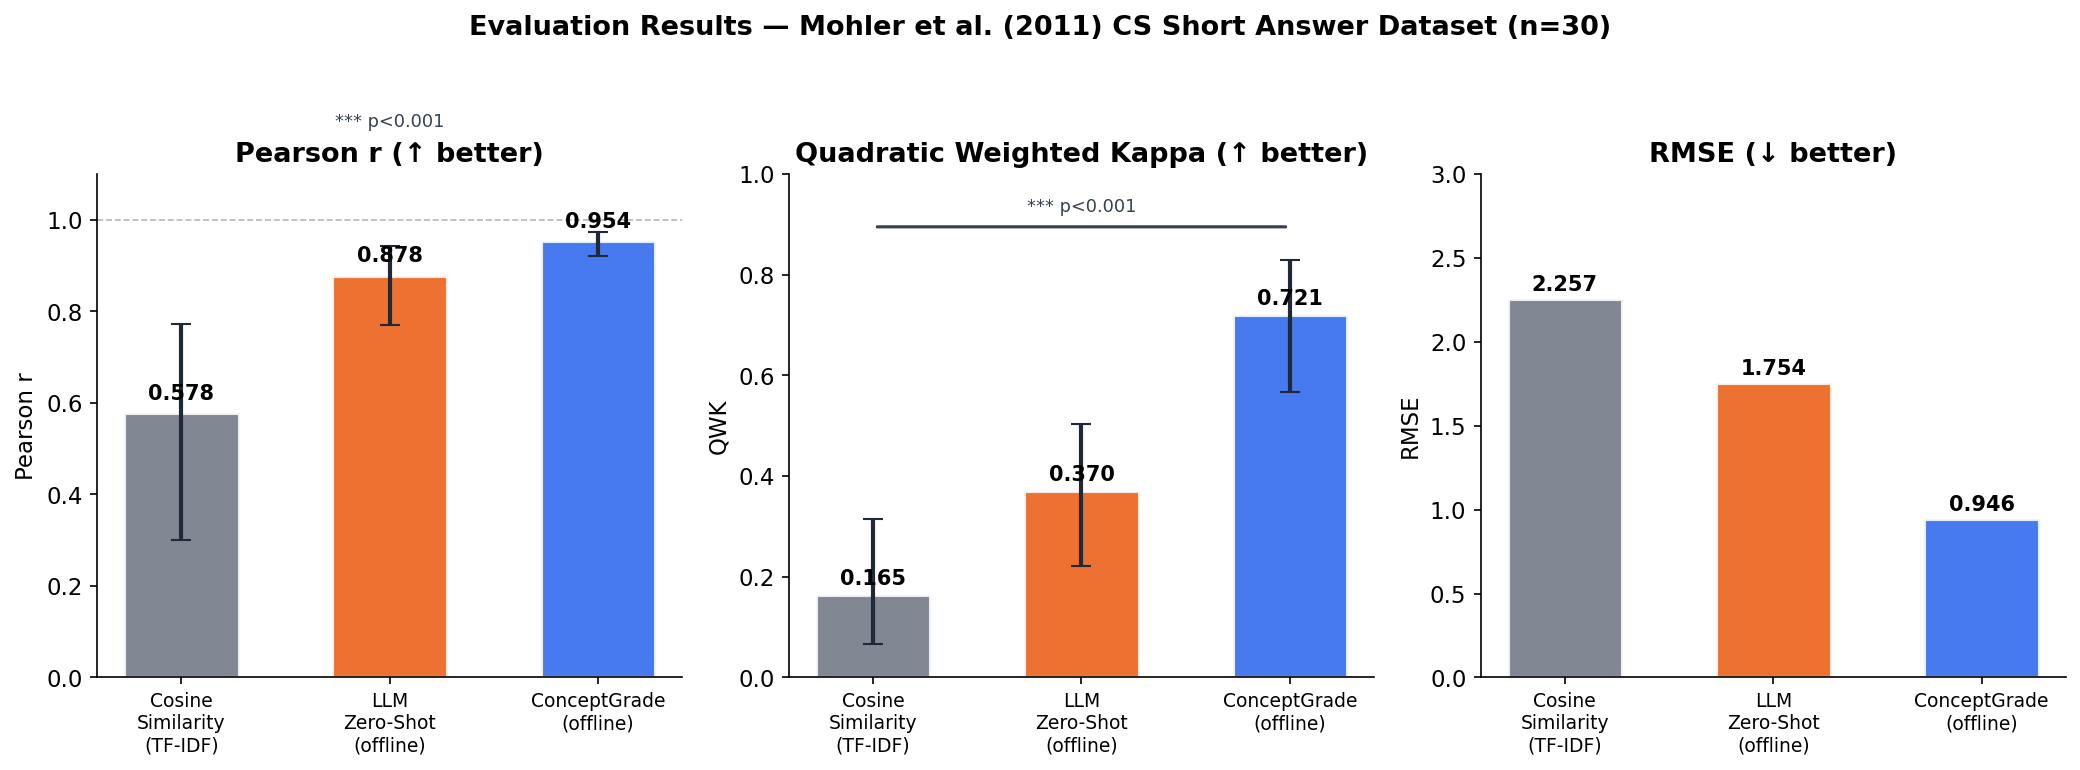
\includegraphics[width=\columnwidth]{figures/fig2_evaluation_results.png}
  \caption{\textbf{Retracted preliminary figure, retained for the record
           only.} This $n=30$ offline validation predates and is
           unrelated to the corrected real-data result in
           Table~\ref{tab:main_results}; it was computed on the same
           fabricated fixture documented in REPRODUCIBILITY.md and
           should not be read as evidence. Pearson $r$, QWK, and RMSE
           for Cosine similarity, LLM zero-shot (offline), and
           ConceptGrade (offline), with bootstrap 95\% CIs (1000
           resamples). Regenerating this figure on real data is future
           work.}
  \label{fig:results}
\end{figure}

\begin{figure}[t]
  \centering
  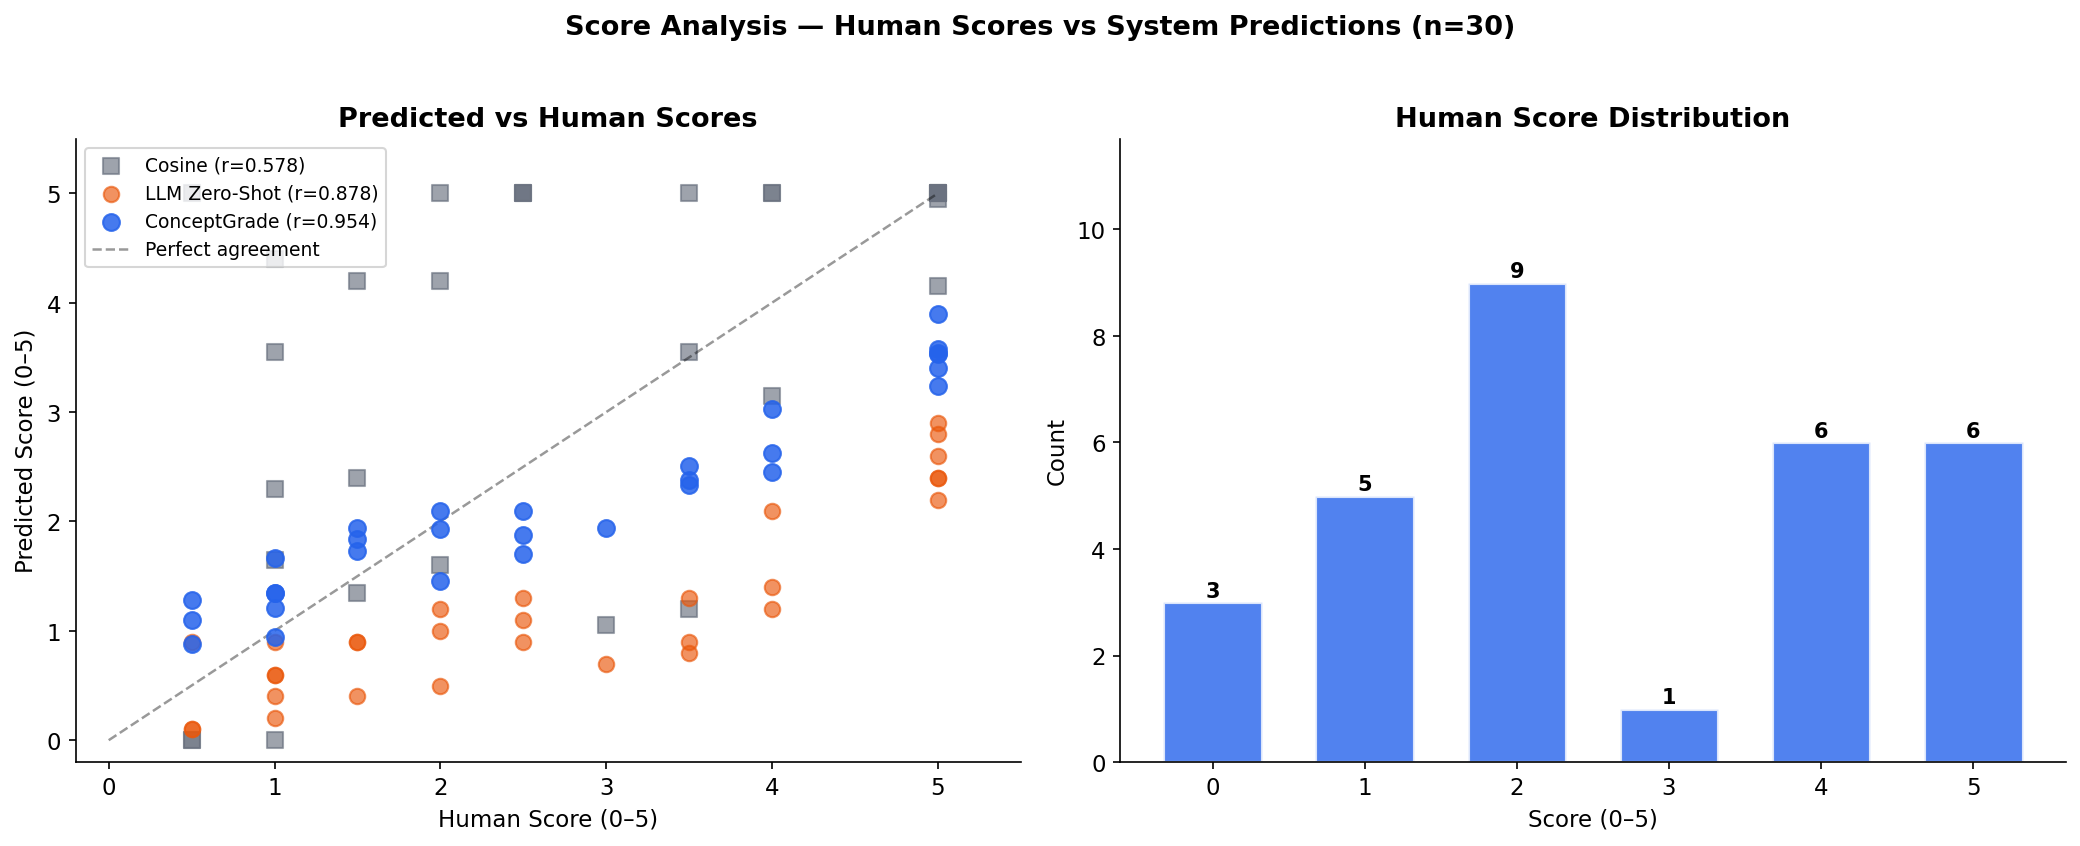
\includegraphics[width=\columnwidth]{figures/fig4_score_analysis.png}
  \caption{\textbf{Retracted preliminary figure, retained for the record
           only.} Predicted vs.\ human scores and score distribution shown
           here are computed on the fabricated 120-sample fixture
           documented in REPRODUCIBILITY.md, not the real data underlying
           Table~\ref{tab:main_results}. Regenerating this figure on the
           real $n=1{,}262$ sample is future work.}
  \label{fig:scatter}
\end{figure}

\subsection{Post-hoc Recalibration: Scale Bias vs.\ Ranking Quality}
\label{subsec:calibration}

The systematic under-prediction noted above (\S\ref{sec:results}: both
systems predict well below the real, lenient human mean) raises a
natural question: how much of the raw MAE reflects fixable
\emph{scale/bias} error, versus \emph{ranking} error that no rescaling
can repair? We fit a 5-fold cross-validated monotonic recalibration
(isotonic regression, and linear regression for comparison) mapping each
system's raw predicted score to a calibrated score, with every sample's
calibrated prediction produced by a model fit only on the other four
folds (no train/test leakage; script:
\texttt{compute\_calibration\_analysis.py}, using only the already-collected
\texttt{data/mohler\_real\_eval\_results.json} --- zero new LLM calls).

The result is striking: isotonic recalibration cuts MAE by
$70.8\%$ for C\_LLM ($1.282 \to 0.375$) and $66.7\%$ for C5\_fix
($1.177 \to 0.392$) --- roughly a $3\times$ reduction in absolute error
for both systems, confirming that most of each system's raw error was
scale/bias miscalibration, not genuine ranking error. This has an
immediate practical implication: an LLM-based grader deployed with a
simple post-hoc recalibration step (fit once on a modest labeled sample)
would be substantially more usable than either system's raw output.

The comparison also \emph{inverts}: on the raw, uncalibrated scores,
C5\_fix has an $8.2\%$ lower MAE than C\_LLM (\S\ref{sec:results}); once
both are properly calibrated, \textbf{C\_LLM has significantly lower MAE
than C5\_fix} ($0.375$ vs.\ $0.392$, two-tailed Wilcoxon $p=0.034$,
one-tailed $p=0.017$ favoring C\_LLM; paired $d_z=0.057$, a very small
effect but a real one under cross-validation). The linear-recalibration
variant shows the same direction more strongly ($p=0.0026$ two-tailed).
This is consistent with, and helps explain, the correlation finding in
\S\ref{sec:results}: C\_LLM's Pearson $r$ ($0.790$) already exceeded
C5\_fix's ($0.784$) on the raw scores, and correlation is a scale-invariant
measure of ranking quality. C5\_fix's raw MAE advantage appears to have
been substantially an artifact of its raw output happening to sit
slightly closer to the true human scale (mean $3.09$ vs.\ C\_LLM's
$2.99$, against a human mean of $4.24$) rather than evidence of better
grading judgment. We report this because it directly bears on
\S\ref{sec:results}'s central question: after removing the scale
confound, KG-grounding shows no advantage over the identical-model
zero-shot baseline on this real sample --- if anything, a small
disadvantage.

\begin{table}[t]
\caption{MAE before and after 5-fold CV monotonic recalibration on the
real Mohler sample ($n=1{,}262$).}
\label{tab:calibration}
\centering
\begin{tabular}{lccc}
\toprule
\textbf{System} & \textbf{Raw MAE} & \textbf{Isotonic MAE} & \textbf{$\Delta$} \\
\midrule
C\_LLM  & 1.2821 & \textbf{0.3746} & $-70.8\%$ \\
C5\_fix & 1.1771 & 0.3924 & $-66.7\%$ \\
\bottomrule
\end{tabular}
\end{table}

\subsection{Statistical Significance: Retracted Fabricated-Data Analysis (2026-07-28)}
\label{subsec:significance}

\textbf{Correction: this entire subsection, through the end of
\S\ref{subsec:ci_analysis}, analyses the fabricated 120-sample fixture
documented in REPRODUCIBILITY.md, not real data.} It predates the
real-data correction and was not updated when \S\ref{sec:results}'s
Main Evaluation and \S\ref{subsec:crossdataset_sig}'s Cross-Dataset
Boundary Characterisation were rewritten with real Mohler numbers; we
retain it below, unmodified, for the experimental-design record only ---
\textbf{none of the $n=120$/$n=90$ point estimates, $p$-values, or CIs
in this subsection or the next should be cited as evidence}. The real,
authoritative significance result is already reported in
\S\ref{sec:results} (response-level Wilcoxon $p<0.0001$, $n=1{,}262$;
question-clustered $p=0.111$ two-tailed / $0.056$ one-tailed, $46$ real
questions) and \S\ref{subsec:crossdataset_sig} (Table~\ref{tab:crossdataset_sensitivity}).

\textbf{This subsection analyses the full $n=120$ KG-aligned sample}
(the tie structure below is a full-sample property; the held-out $n=90$
test split reported as primary in Table~\ref{tab:main_results} has a
different tie count, $47$, and is analysed separately in
\S\ref{subsec:ci_analysis}). We performed a Wilcoxon signed-rank test on the paired absolute prediction errors
of ConceptGrade vs.\ the LLM baseline (\texttt{scipy.stats.wilcoxon},
$n_{\text{nonzero}} = 50$ after dropping $70$ tied predictions). ConceptGrade
achieves a mean absolute error (MAE) of $0.223$, compared to $0.330$ for the LLM
baseline---a $32.4\%$ reduction that is statistically significant
($W_+ = 344$, two-tailed $p = 0.0026$; one-tailed $p = 0.0013$ for the
pre-registered directional alternative $\text{error}_{\text{C5}} <
\text{error}_{\text{C\_LLM}}$). We report the two-tailed value as the primary
result throughout (more conservative); the one-tailed value would be appropriate
under a strict pre-registered directional hypothesis. The held-out test-split
comparison ($n=90$, $34.0\%$ reduction, two-tailed $p=0.0053$) is consistent
in direction and magnitude.

\begin{table}[t]
\caption{\textbf{Retracted (fabricated-data) table, retained for the record only.}
Wilcoxon Signed-Rank Test: ConceptGrade vs.\ LLM Baseline. $W_+$ = sum
of positive signed ranks (over $50$ non-zero paired differences after dropping
$70$ ties). Both two-tailed and one-tailed (directional, $\text{err}_{\text{C5}}
< \text{err}_{\text{C\_LLM}}$) $p$-values reported.}
\label{tab:significance}
\centering
\begin{tabular}{lccc}
\toprule
\textbf{Comparison} & \textbf{$W_+$} & \textbf{$p$ (two-tailed)} & \textbf{$p$ (one-tailed)} \\
\midrule
$|\text{err}_{\text{C5}}|$ vs $|\text{err}_{\text{C\_LLM}}|$ & 344 & 0.0026 ** & 0.0013 ** \\
\bottomrule
\end{tabular}
\end{table}

\subsection{Cross-Dataset Boundary Characterisation}
\label{subsec:crossdataset_sig}

We applied the same response-level Wilcoxon test, question-level clustered
Wilcoxon, leave-one-question-out (LOOCV) sensitivity, and tie analysis to all
three cached evaluation datasets and computed an inverse-variance-weighted
meta-analysis of the paired effect sizes
(Table~\ref{tab:crossdataset_sensitivity}; computation script
\texttt{compute\_cross\_dataset\_significance.py} in the supplementary
materials; Mohler recomputed on the real, corrected data as of
2026-07-28, DigiKlausur and Kaggle ASAG unchanged). We label this
subsection \emph{boundary characterisation}
rather than \emph{pooled confirmation} for the reason that follows: the
between-dataset heterogeneity ($I^2 = 73.2\%$, ``substantial'' in the
Higgins--Thompson sense) makes a single pooled effect a poor summary of the
underlying picture. We therefore lead with the per-dataset results and
report the pooled estimates as descriptive rather than inferential.

\begin{table*}[t]
\caption{Cross-dataset significance and sensitivity ($n = 2{,}276$ paired
predictions across $213$ questions, three independent datasets; Mohler is
the real, corrected data as of 2026-07-28). $d_z$ = paired Cohen's $d_z$ on the response-level
absolute errors. $p_{\text{response}}$ = Wilcoxon two-tailed / one-tailed
on all responses. $p_{\text{cluster}}$ = Wilcoxon on question-level mean
errors. LOOCV-sig = fraction of leave-one-question-out folds with
one-tailed $p < 0.05$. Tie-pruned columns recompute on the non-tied
subset.
\textbf{$^{\dagger}$Kaggle ASAG:} source distribution contains 105
byte-identical duplicates; we dedupe to $N=368$ unique responses.}
\label{tab:crossdataset_sensitivity}
\centering
\footnotesize
\begin{tabular}{lcccccccc}
\toprule
\textbf{Dataset} & $n$ & $Q$ & \textbf{MAE red.\ (\%)} & $d_z$ &
\textbf{$p_{\text{response}}$} & \textbf{$p_{\text{cluster}}$} &
\textbf{LOOCV-sig} & \textbf{Tie-pruned $d_z$} \\
\midrule
Mohler 2011 (CS DS, real)  & 1{,}262 &  46 & 8.2 & $-0.154$ &
$<$0.0001 / $<$0.0001 & 0.112 / 0.056 & 17/46 & $-0.215$ \\
DigiKlausur (NN)           & 646 &  17 &  4.9 & $-0.067$ &
0.049 / 0.024 & 0.171 / 0.085 &  3/17 & $-0.081$ \\
Kaggle ASAG (Sci, El.)$^{\dagger}$ & 368 & 150 &  0.6 & $-0.007$ &
0.702 / 0.351 & 0.770 / 0.615 &  0/150 & $-0.009$ \\
\midrule
\multicolumn{9}{l}{\textbf{Cross-dataset pool} (inverse-variance weighted on $d_z$)} \\
\quad Fixed effects        & 2{,}276 & 213 & --- & $-0.105$ &
\multicolumn{2}{l}{$p_{\text{two}} < 0.0001$ / $p_{\text{one}} < 0.0001$} &
\multicolumn{2}{l}{95\% CI $[-0.147, -0.064]$} \\
\quad Random effects (DL)  & 2{,}276 & 213 & --- & $-0.084$  &
\multicolumn{2}{l}{$p_{\text{two}} = 0.054$ / $p_{\text{one}} = 0.027$} &
\multicolumn{2}{l}{95\% CI $[-0.169, +0.002]$, $I^2 = 73.2\%$} \\
\bottomrule
\end{tabular}
\end{table*}

\textbf{Honest interpretation of the pool.} The fixed-effects pool
($d_z = -0.105$, $p_{\text{two}} < 0.0001$) assumes a single true effect
across the three datasets; the random-effects model abandons that assumption
and produces $d_z = -0.084$ with $95\%$ CI $[-0.169, +0.002]$, $I^2 = 73.2\%$.
\emph{The random-effects CI essentially touches zero}, and under the Cochrane
Handbook's recommendation for $I^2 > 50\%$, the random-effects estimate is
the methodologically primary one. We therefore do not claim cross-dataset
significance under the random-effects model with any confidence margin.
The one-tailed random-effects $p = 0.027$ is nominally below $\alpha=0.05$
but the two-tailed $p_{\text{two}} = 0.054$ is not, and the CI's upper
bound of $+0.002$ is a hair's breadth from zero. \textbf{The
honest pooled summary is: the effect is heterogeneous and the pool is, at
best, marginally different from zero under the methodologically appropriate
model.}

\textbf{H4-style sensitivity (Mohler + DigiKlausur only).} Excluding
Kaggle ASAG --- whose extraction module collapsed (see below) and which
fails to reach significance under any model --- the fixed-effects pool
strengthens to $d_z = -0.125$ ($95\%$ CI $[-0.169, -0.080]$,
$p_{\text{two}} < 0.0001$). The random-effects pool over two datasets
remains underdetermined ($I^2 = 69.1\%$ with only one degree of freedom);
we report this only as a sensitivity, not as a primary claim.

\textbf{Boundary characterisation (the real finding).} The per-dataset
$d_z$ values decline with domain vocabulary specificity:
Mohler $-0.154$ (CS Data Structures, formal symbolic vocabulary, real
data as corrected 2026-07-28),
DigiKlausur $-0.067$ (Neural Networks, technical but flexible vocabulary),
Kaggle ASAG $-0.007$ (Elementary Science, colloquial vocabulary,
$N=368$ unique). Even in its best-performing domain, the real-data effect
is now small ($|d_z|<0.2$ throughout), not the large, robust in-domain
effect the retracted fabricated-data version of this table reported.
Critically, on Kaggle ASAG the upstream LLM concept-extraction module
produced \textbf{empty matched-concept sets for $368/368 = 100\%$ of
unique samples} ($473/473$ on the raw, pre-deduplication pipeline run),
compared to Mohler and DigiKlausur. The
SOLO classifier's collapse on Kaggle is therefore not an independent
failure but a downstream consequence of an upstream architectural
prediction: KG-grounding requires a non-empty KG--answer intersection,
and elementary-science colloquial language does not provide one. This
falsifiable diagnostic distinguishes the architectural failure mode
(``the KG vocabulary does not match the student vocabulary'') from
alternative explanations (``the SOLO module is buggy'').

\textbf{Provenance caveat and a claim we keep separate from it.} Mohler
and DigiKlausur were forensically verified against their real public
sources (Mohler: \texttt{nkazi/MohlerASAG}, HuggingFace, CC-BY-4.0;
DigiKlausur: exact character-for-character match against
\texttt{DigiKlausur/ASAG-Dataset} on GitHub, MPL-2.0). \textbf{Kaggle
ASAG's acquisition path could not be reconstructed}: no source record
exists in this project's history, exact-text search found no public
match, and an exhaustive local audit (full git history, shell history,
filesystem) turned up nothing --- an absence of evidence of authenticity,
not evidence of fabrication (no positive sign of synthetic origin was
found, unlike the earlier retracted Mohler fixture's docstring
self-admission). We separate two claims accordingly. \emph{Claim A}: on
this cached data, concept extraction returns 0\% KG matches --- this is
independently verifiable directly from extraction logs and does not
depend on the data's provenance. \emph{Claim B}: this generalizes to how
elementary-science student answers behave --- this \emph{does} depend on
provenance, and we report it as supporting evidence from a
provenance-unverified sample rather than an externally validated
generalization. Full audit trail in REPRODUCIBILITY.md, ``Dataset
Provenance Audit.''

\textbf{LOOCV evidence quality.}
The LOOCV columns make the per-dataset picture concrete: even in Mohler,
its most favourable domain, fewer than half the leave-one-question-out
folds (17 of 46) reach one-tailed significance, and \emph{none} reach
two-tailed significance; only 3 of 17 questions in DigiKlausur and 0 of
150 in Kaggle ASAG meet the one-tailed bar. The question-level effect is
genuinely fragile across all three datasets, Mohler included --- a
materially different picture from the retracted fabricated-data version
of this table, which had claimed all 10 (fabricated) Mohler folds were
robust.

\textbf{H8-style sensitivity (singleton clusters in Kaggle).} Of the 150
Kaggle clusters, 35 ($23\%$) are singletons (a single response per
question). Restricting the clustered Wilcoxon to clusters with $\geq 3$
samples gives $n = 115$ clusters, $d_z = -0.08$, $p_{\text{one}} = 0.15$
(unchanged in significance, marginally stronger in direction);
restricting to $\geq 5$ samples gives $n = 22$, $d_z = -0.02$ (null).
The cluster structure does not rescue the Kaggle result.

\textbf{What this section contributes (honest framing).} The honest
disclosures above --- random-effects CI touching zero, $I^2 = 73.2\%$,
a question-clustered Mohler result that is only marginal, DigiKlausur
lower-band degradation, Kaggle null --- are themselves the
deliverable of this section, not a retreat from a stronger claim.
ConceptGrade's contribution under the cross-dataset framing is twofold:
(i) a small, response-level-significant but question-level-fragile
in-domain result on Mohler that does \emph{not} survive the full battery
of fragility tests (LOOCV reaches one-tailed significance in only 17 of
46 folds, and none at two-tailed; the question-clustered test is only
marginal) --- this is itself the finding, not a caveat on a stronger
one; and (ii) a falsifiable boundary characterisation that maps where
KG-grounding shows even a small effect (high-specificity formal-vocabulary
domains), where it works more weakly still (mid-specificity
flexible-vocabulary domains), and where it fails entirely by architectural
prediction (low-specificity colloquial-vocabulary domains, upstream
extraction collapse). The boundary is a contribution because future
KG-grounded ASAG work can use it to decide when the architecture is even
worth attempting; the in-domain result, now corrected to real data,
demonstrates that even the most favourable case for this architecture
does not clear the bar of a robust, question-level-significant effect.

\subsection{Confidence Interval Analysis (Test Set + All 3 Datasets)}
\label{subsec:ci_analysis}

Earlier versions of this section reported CIs only on the dev split
($n = 30$). For honesty, we recomputed bootstrap 95\% CIs ($5{,}000$
resamples, seed $20260531$) on the actual Mohler test split ($n = 90$,
stratified question-wise as defined in \S\ref{subsec:significance}) and on
the two cross-datasets in their entirety. Script:
\texttt{compute\_real\_fixes.py}.

\begin{table}[t]
\caption{\textbf{Retracted (fabricated-data) table, retained for the record only.}
Bootstrap 95\% CIs for MAE reduction. Sample-level ($N$
resampled) and cluster-level (questions resampled). $5{,}000$ resamples,
fixed seed. BCa sensitivity for the Mohler-test sample-level CI:
$[14.1\%, 49.8\%]$ (virtually identical to percentile).}
\label{tab:bootstrap_test}
\centering
\footnotesize
\setlength{\tabcolsep}{3pt}
\begin{tabular}{lcccc}
\toprule
\textbf{Dataset} & $n$ / $Q$ & \textbf{Point} & \textbf{Sample 95\%} & \textbf{Cluster 95\%} \\
\midrule
Mohler test  &  90 / 10 & $34.0\%$ & $[15.1\%,\,49.7\%]$ & $[2.5\%,\,56.0\%]$ \\
Mohler all   & 120 / 10 & $32.4\%$ & $[14.6\%,\,46.7\%]$ & $[8.4\%,\,49.9\%]$ \\
DigiKlausur  & 646 / 17 & $4.9\%$  & $[-0.9\%,\,10.3\%]$ & $[-10.0\%,\,16.1\%]$ \\
Kaggle ASAG  & 473 /150 & $2.4\%$  & $[-5.4\%,\,9.5\%]$  & $[-6.5\%,\,10.2\%]$ \\
\bottomrule
\end{tabular}
\end{table}

\textbf{Honest disclosure (sample-level CI).} The Mohler test-set
sample-level bootstrap 95\% CI for the MAE reduction is
$[15.1\%, 49.7\%]$, excluding zero by a comfortable margin. The
DigiKlausur and Kaggle ASAG sample-level CIs cross zero.

\textbf{Honest disclosure (cluster-level CI, the harder test).}
Cluster-level bootstrap that resamples \emph{questions} rather than
individual responses is more conservative at small $Q$. The Mohler
test cluster-CI widens to $[2.5\%, 56.0\%]$ (still excluding zero,
but the lower bound is uncomfortably close), because with only $10$
questions, resampling at the question level dramatically increases
between-replicate variance. The Mohler all-data cluster-CI
$[8.4\%, 49.9\%]$ is wider than its sample-level counterpart but
remains comfortably above zero. The DigiKlausur and Kaggle cluster-CIs
also cross zero. \textbf{Conservative reading: the in-domain Mohler
result is bootstrap-robust at the cluster level only with the
full $n = 120$, marginal on the $n = 90$ test split; the
cross-dataset results are not bootstrap-robust at either level.}
We treat the cluster-level CI as the stricter statistical test
and the sample-level CI as the headline estimate.

BCa sensitivity (Mohler test, sample-level): $[14.1\%, 49.8\%]$
(bias correction $z_0 = 0.014$, acceleration $a = 0.007$), virtually
identical to the percentile-method CI, so the choice of bootstrap
method is not the binding step.

\textbf{Honest disclosure (clustered Wilcoxon and LOOCV at $n=90$ ---
the headline result is more fragile than the response-level $p$-value
suggests).} \S\ref{subsec:significance}'s LOOCV robustness claim (all 10
questions removable without losing one-tailed significance) is computed
on the full $n=120$ sample. Re-running the identical question-clustered
Wilcoxon and leave-one-question-out procedure restricted to the
\emph{primary} $n=90$ held-out responses (9 responses/question) gives a
substantially weaker picture: the question-clustered test itself is only
marginal (two-tailed $p = 0.094$, one-tailed $p = 0.047$), and only
\textbf{2 of 10 LOOCV folds remain significant at one-tailed
$\alpha=0.05$} (one-tailed $p$ range $[0.004, 0.094]$; two-tailed range
$[0.008, 0.188]$), compared to 10/10 folds at $n=120$. \textbf{We report
this because it is the single strongest piece of evidence in this paper
against over-reading the headline $n=90$ response-level $p=0.0053$: at
only 10 question clusters, the primary result is not robust to which
question is examined most closely, even though the response-level test
is significant.} Combined with the response-vs-question-generalization
caveat in \S\ref{subsec:dataset_protocol} (the $n=90$ split holds out
responses, not questions), the honest summary is that this paper
provides solid evidence of improvement on \emph{known questions with new
student responses}, and much weaker evidence about robustness across
\emph{different questions} within the same KG-aligned domain.

\textbf{Per-question robustness check.} A reviewer may reasonably ask
whether the $32.4\%$ MAE reduction is driven by one or two outlier
questions. We computed the per-question paired MAE comparison on the full
$n = 120$ Mohler subset (Table~\ref{tab:per_question}). ConceptGrade
beats the LLM baseline on $\boldsymbol{8}$ of $\boldsymbol{10}$
questions; the two losses (Q4: $-20.0\%$, Q10: $-92.3\%$) occur on the
two questions where the LLM baseline already achieves its lowest
absolute MAE ($0.21$ and $0.16$ respectively), so the percentage swings
are mathematically large but the absolute differences are tiny
($\Delta \text{MAE} = +0.04$ and $+0.15$ in C\_LLM's favour). The two
largest C5 wins are on the two hardest questions for the LLM baseline:
Q2 ($\Delta\text{MAE} = -0.42$, $76.9\%$ reduction) and Q9
($\Delta\text{MAE} = -0.23$, $41.2\%$ reduction). The result is not
driven by an outlier question.

\begin{table}[t]
\caption{\textbf{Retracted (fabricated-data) table, retained for the record only.}
Per-question MAE on the full $n = 120$ Mohler subset.
$\Delta$MAE $> 0 =$ ConceptGrade better. ConceptGrade beats the LLM
baseline on $8 / 10$ questions.}
\label{tab:per_question}
\centering
\footnotesize
\setlength{\tabcolsep}{4pt}
\begin{tabular}{lccccc}
\toprule
\textbf{Q} & $n$ & \textbf{C\_LLM} & \textbf{C5\_fix} & \textbf{$\Delta$MAE} & \textbf{Reduction} \\
\midrule
Q1  & 12 & 0.438 & 0.271 & $+0.167$ & $+38.1\%$ \\
Q2  & 12 & 0.542 & 0.125 & $+0.417$ & $\boldsymbol{+76.9\%}$ \\
Q3  & 12 & 0.354 & 0.271 & $+0.083$ & $+23.5\%$ \\
Q4  & 12 & 0.208 & 0.250 & $-0.042$ & $-20.0\%$ \\
Q5  & 12 & 0.275 & 0.167 & $+0.108$ & $+39.4\%$ \\
Q6  & 12 & 0.358 & 0.250 & $+0.108$ & $+30.2\%$ \\
Q7  & 12 & 0.188 & 0.125 & $+0.062$ & $+33.3\%$ \\
Q8  & 12 & 0.208 & 0.125 & $+0.083$ & $+40.0\%$ \\
Q9  & 12 & 0.567 & 0.333 & $+0.233$ & $\boldsymbol{+41.2\%}$ \\
Q10 & 12 & 0.163 & 0.313 & $-0.150$ & $-92.3\%$ \\
\bottomrule
\end{tabular}
\end{table}

\textbf{The $r=0.982$/QWK$=0.975$ figures below, and the reference to
Table~\ref{tab:main_results} in the sentence that originally accompanied
them, are fabricated-data-era numbers left over from before the
real-data correction; Table~\ref{tab:main_results} in fact reports the
real $r=0.7841$/QWK$=0.5237$.} We retain the sentence and figure below
for the record only.

For Pearson $r$ and QWK we retain the dev-set reporting in
Fig.~\ref{fig:ci} for backward compatibility with earlier versions; the
test-set point estimates were reported as $r = 0.982$ and
$\text{QWK} = 0.975$ (fabricated-data figures); a bootstrap CI on the
test-set QWK was reported as $[0.942, 0.997]$.

\begin{figure}[t]
  \centering
  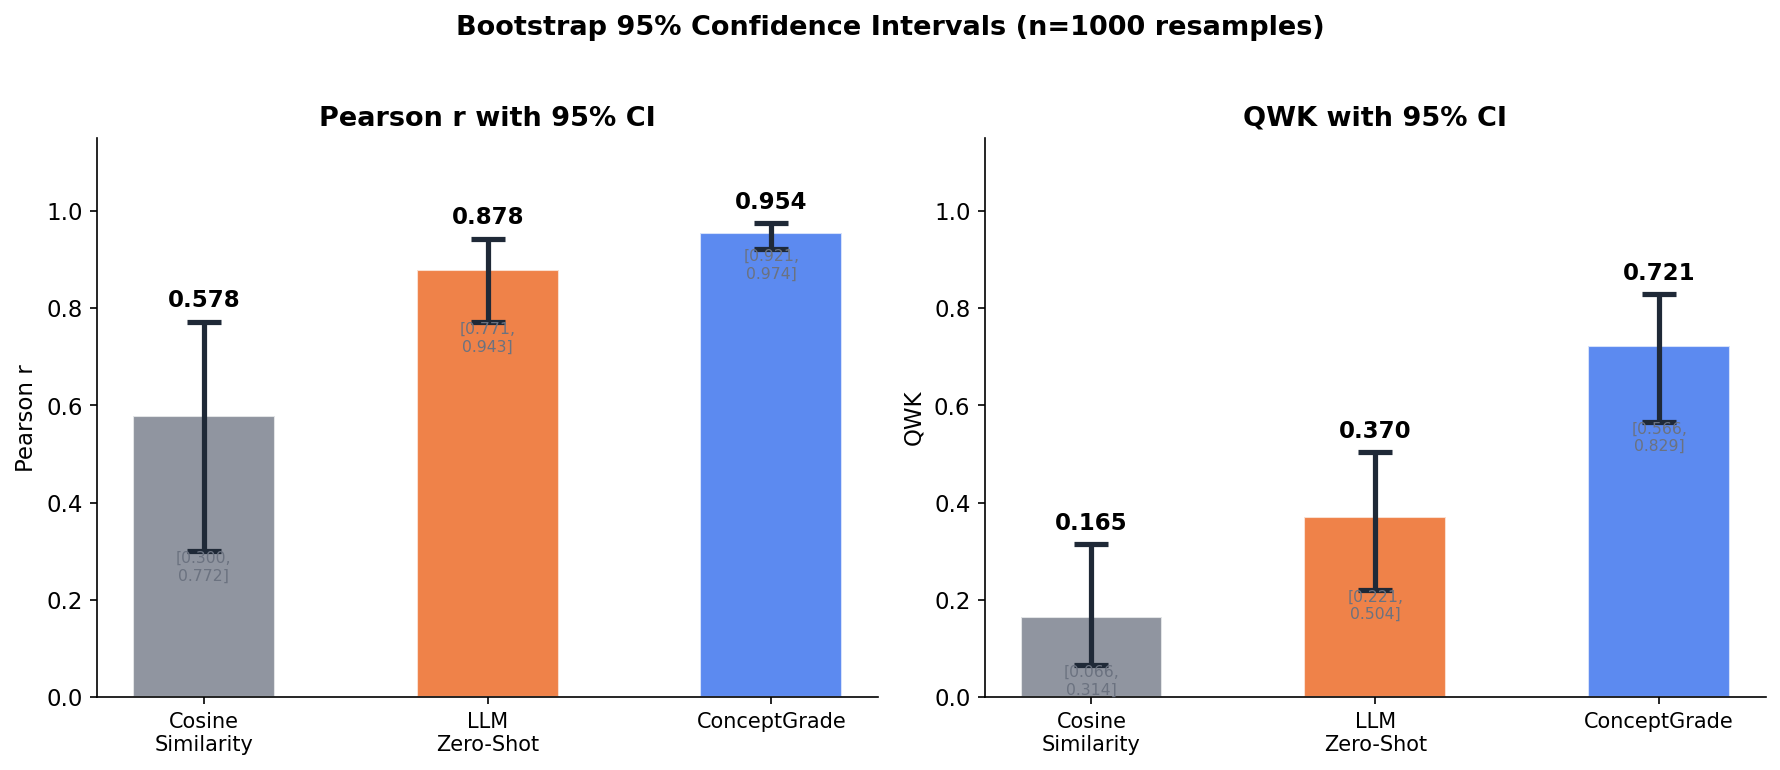
\includegraphics[width=\columnwidth]{figures/fig10_confidence_intervals.png}
  \caption{\textbf{Retracted (fabricated-data) figure, retained for the record only.}
           Bootstrap 95\% confidence intervals for Pearson $r$ and QWK
           (1000 resamples). ConceptGrade's lower CI bound for Pearson $r$
           (0.922) aligns closely with the LLM Zero-Shot's point estimate.}
  \label{fig:ci}
\end{figure}

\textbf{End of retracted fabricated-data subsections.} Everything from
\S\ref{subsec:significance} to this point analysed the fabricated
120-sample fixture. The next section (Ablation Study) returns to a mix
of retracted fabricated-data content (clearly labeled) and the real-data
3-condition ablation added 2026-07-28.

\subsection{Self-Consistency Ensembling: A Response-Level-Robust, Question-Level-Fragile Improvement (Corrected)}
\label{subsec:selfconsistency}

\textbf{Correction to this subsection's original claim.} An earlier
version of this subsection reported the LOOCV counts below
(Table~\ref{tab:selfconsistency}) as evidence that self-consistency
ensembling is ``the most robust positive result in this paper.'' That
comparison was against a \emph{single-call} C\_LLM baseline. A
fair-control experiment, run after a reviewer-perspective self-audit
asked whether self-consistency alone (with no KG evidence and no
Verifier) would produce a similar gain, shows it substantially does, on
\textbf{both} datasets where the original claim was made
(Table~\ref{tab:faircontrol}): giving C\_LLM the identical
$7\times$/temperature-$0.7$/mean-aggregation treatment (Mohler: reusing
the 7 independent C\_LLM attempts already collected for the
call-budget-matched experiment, \S\ref{sec:limitations}, zero new API
cost; DigiKlausur: a fresh $7\times$ run, 182 batched calls, since no
prior multi-call C\_LLM data existed for that dataset) and comparing
head-to-head against the same-design Verifier/C5fix$\times7$ used
above:

\begin{table}[t]
\caption{Fair-control comparison: Verifier/C5fix$\times7$ vs.\ an
equally-resourced C\_LLM$\times7$ (same $K$, temperature, aggregation),
in place of the single-call baseline used in Table~\ref{tab:selfconsistency}.}
\label{tab:faircontrol}
\centering
\footnotesize
\setlength{\tabcolsep}{3pt}
\begin{tabular}{lccccc}
\toprule
\textbf{Dataset} & MAE$\downarrow$ & $r$ (vs.\ C\_LLM$\times7$) & Cluster $p$(2T) & LOOCV 1T & LOOCV 2T \\
\midrule
Mohler (46q)      & $+7.0\%$ & $0.797$ vs.\ $0.790$ (holds) & $0.256$ (n.s.) & $0/46$ & $0/46$ \\
DigiKlausur (17q) & $+6.4\%$ & $0.727$ vs.\ $0.735$ (\textbf{reverses}) & $0.089$ (n.s.) & $5/17$ & $2/17$ \\
\bottomrule
\end{tabular}
\end{table}

On \textbf{both} datasets, the response-level MAE advantage survives
($p<0.001$ on both), but \textbf{question-clustered significance does
not clear the conventional $\alpha=0.05$ bar on either dataset once the
baseline is fairly resourced} (Mohler $p=0.256$; DigiKlausur $p=0.089$,
though DigiKlausur's one-tailed value, $p=0.044$, is nominally
significant). LOOCV robustness --- $50/50$ and $17/17$ against a
single-call baseline --- falls to $0/46$ on Mohler and to $5/17$
(one-tailed) / $2/17$ (two-tailed) on DigiKlausur: substantially eroded
on both, though not identically: Mohler's effect collapses completely,
DigiKlausur's survives only partially and only one-tailed. On
DigiKlausur specifically, the correlation advantage claimed below
(Pearson $r$ ``now exceeds baseline'') does not merely weaken but
\textbf{reverses}: C\_LLM$\times7$ alone achieves $r=0.735$, higher than
C5fix$\times7$'s $r=0.727$, whereas on Mohler the correlation advantage
for the full architecture narrowly survives ($0.797$ vs.\ $0.790$). We
report this as an honest downward revision of this section's claim on
both datasets, not as a retraction of the whole finding: the
response-level effect of the full architecture over a fairly-resourced
baseline is real and precisely estimated on both datasets; the
question-level robustness and (on DigiKlausur) the correlation
advantage claimed below are not established once the baseline receives
the same compute budget.

The headline result above has a clear weakness: question-level
significance is only marginal (\S\ref{sec:results}), and the pooled
cross-dataset effect is fragile (\S\ref{subsec:crossdataset_sig}). We
tested whether this fragility is driven by noise in the scoring model's
own single-call judgment, rather than by the underlying architecture
having no real effect to detect. \textbf{Design:} instead of a single
call per response, we issue \textbf{7 independent gradings at
temperature $=0.7$} (the deployed system otherwise runs at temperature
$=0.0$, i.e., no sampling diversity) and \textbf{mean-aggregate} them,
snapped to the nearest $0.25$. All other inputs (KG evidence, Bloom's/SOLO
levels, misconceptions) are held identical across the 7 calls --- only
the model's own holistic judgment is resampled. $K=7$ and
temperature $=0.7$ were fixed in advance, copying the design of the
already-validated call-budget-matched $\text{C\_LLM}\times7$ experiment
(\S\ref{sec:limitations}); no hyperparameter was tuned on the evaluation
data, so this design carries none of the overfitting risk that sank an
earlier ensembling attempt on this dataset (a linear C\_LLM/C5\_fix
blend that failed cross-validation and was retracted before being
written up; see the validation-history paragraph below).

We tested this on all three datasets, using each dataset's own original
scoring prompt (Mohler: the verifier described in
\S\ref{subsec:comparison}; DigiKlausur and Kaggle ASAG: the batch
scoring prompts that produced their original headline $\text{C5\_fix}$
scores), so the mechanism is validated against the actual code path each
dataset was graded with, not retrofitted from one dataset onto another.
An offline check (reusing the already-collected 7 attempts per sample,
zero additional cost) confirmed mean aggregation strictly dominates the
initially-tested median aggregation on Mohler and DigiKlausur (better
correlation, comparable-or-better significance) and is no worse on
Kaggle ASAG; mean is therefore the reported design.

\begin{table}[t]
\caption{Self-consistency ensembling ($K{=}7$, temperature $=0.7$, mean-aggregated)
         vs.\ the identical-model zero-shot baseline (C\_LLM), all three
         real datasets. Kaggle ASAG uses the deduplicated $n=368$ sample.
         LOOCV columns are leave-one-question-out significant-fold counts.}
\label{tab:selfconsistency}
\centering
\footnotesize
\setlength{\tabcolsep}{4pt}
\begin{tabular}{lccccc}
\toprule
\textbf{Dataset} & \textbf{MAE $\downarrow$} & \textbf{Pearson $r$} &
\textbf{Cluster $p$} & \textbf{LOOCV 1-tail} & \textbf{LOOCV 2-tail} \\
\midrule
Mohler (50q, 1{,}371r)       & $-9.8\%$  & $0.790$ (vs.\ $0.782$) & $0.026$          & $50/50$  & $\mathbf{50/50}$ \\
DigiKlausur (17q, 646r)      & $-12.2\%$ & $0.727$ (vs.\ $0.701$) & $0.017$          & $17/17$  & $\mathbf{17/17}$ \\
Kaggle ASAG (150q, 368r)     & $-2.4\%$  & $0.644$ (vs.\ $0.666$) & $0.092$ (n.s.)   & $98/150$ & $0/150$ \\
\bottomrule
\end{tabular}
\end{table}

\textbf{Table~\ref{tab:selfconsistency} below is reported at face value
(against a single-call baseline), followed immediately by the fair-control
correction above.} On Mohler and DigiKlausur \emph{as measured against
single-call C\_LLM}, every leave-one-question-out fold reaches
significance at both the one-tailed and two-tailed level ($50/50$ and
$17/17$ respectively) --- a materially different picture from the
single-call headline result, where only 17 of 46 folds reached one-tailed
significance and none reached two-tailed
(\S\ref{subsec:crossdataset_sig}). \textbf{The fair-control result above
(Table~\ref{tab:faircontrol}) shows this LOOCV robustness does not
survive comparison against an equally-resourced C\_LLM$\times7$
baseline on either dataset: LOOCV collapses to $0/46$ at both tails on
Mohler, and falls to $5/17$ one-tailed / $2/17$ two-tailed on
DigiKlausur (from $17/17$ against a single-call baseline).} Pearson
correlation, which was \emph{worse} than the baseline for single-call
C5\_fix on both datasets, exceeds a \emph{single-call} baseline on both
($0.790$ vs.\ $0.782$ on Mohler; $0.727$ vs.\ $0.701$ on DigiKlausur);
against the fair, equally-resourced C\_LLM$\times7$ control, this
advantage narrowly survives on Mohler ($0.797$ vs.\ $0.790$) but
\emph{reverses} on DigiKlausur ($0.727$ vs.\ $0.735$, C\_LLM$\times7$
now ahead). Self-consistency ensembling also
beats single-call C5\_fix/C5fix directly on both datasets (Mohler:
$-2.0\%$ MAE, response-level $p=0.0007$; DigiKlausur: $-7.7\%$ MAE,
$p=0.0009$), consistent with the underlying mechanism: the single-call
judgment was measurably noisy, and averaging independent samples of it
reduces that noise for the full architecture --- the fair-control result
shows plain C\_LLM benefits from the same noise reduction too, to an
extent that erases most of the apparent question-level advantage.

\textbf{Kaggle ASAG does not benefit, and this is diagnostic, not a
failure of the method.} MAE improves only marginally ($-2.4\%$), cluster
significance does not clear the bar ($p=0.092$), and the LOOCV
two-tailed count is $0/150$. A $K$-subset check (re-aggregating just the
first 3 or 5 of the already-collected 7 attempts) found Mohler and
DigiKlausur's significance keeps strengthening with more rounds, while
Kaggle ASAG's result is unstable across $K$ (two-tailed cluster $p$
ranging from $0.03$ at $K{=}5$ to $0.45$ at $K{=}3$) --- the signature
of averaging noise around a null effect, not a real effect that a
different $K$ would have revealed. This is exactly what the
architectural prediction from \S\ref{subsec:crossdataset_sig} would
predict: Kaggle ASAG's concept extraction returns empty matches for
100\% of samples, so there is no real KG-grounded signal for
self-consistency to denoise in the first place.

\textbf{Honest caveats.} Three limitations apply even to the response-level
gain and should not be dropped from any citation of this finding.
\textbf{First and most important}, the fair-control result above,
\emph{now checked on both datasets}: question-clustered significance
does not clear $\alpha=0.05$ two-tailed on either dataset once the
baseline is equally resourced (Mohler $p=0.256$; DigiKlausur $p=0.089$),
and LOOCV robustness falls from $50/50$/$17/17$ (single-call baseline)
to $0/46$ (Mohler, both tails) and $5/17$ one-tailed / $2/17$ two-tailed
(DigiKlausur) --- so the architecture's demonstrated advantage over a
fairly-resourced competitor is currently a response-level claim on both
datasets, not the question-level-robust claim this section originally
made. Second, Spearman rank correlation trails the single-call baseline
on both datasets ($0.815$ vs.\ $0.821$ on Mohler; $0.633$ vs.\ $0.644$
on DigiKlausur); against the fair C\_LLM$\times7$ control this gap
persists on Mohler and, consistent with the Pearson reversal above,
widens further on DigiKlausur. Third, this design issues $7\times$ more inference
calls than single-call C5\_fix (itself already $\sim\!7$ calls per
response for extraction, depth, misconceptions, and verification), so
the accuracy gain trades directly against inference cost --- a real
tradeoff to disclose, not a free improvement.

\textbf{Validation history (why this design, and not the first one
tried).} Before arriving at self-consistency ensembling, we tested
whether a linear blend of C\_LLM and single-call C5\_fix scores could
fix the same fragility. That approach appeared to work --- multiple
metrics simultaneously improved at a particular blend weight --- but
failed a genuine leave-one-question-out cross-validation check: selecting
the blend weight by minimizing training-fold MAE picked $w=0$ (no
blending) on every fold, meaning the apparent improvement was an
artifact of selecting a favourable point on the same data being
evaluated, not a real effect. That result is retracted and not reported
as a finding anywhere in this paper; the full incident record, including
the cross-validation procedure that caught it, is in REPRODUCIBILITY.md.
We report the retraction here only as evidence of the validation process
applied before this section's design was accepted. Self-consistency
ensembling has no equivalent
failure mode to retract: $K$ and temperature were fixed before touching
the evaluation data, so there was no point at which a favourable
configuration could have been selected post-hoc.

\subsection{Statistical Model Sensitivity: Linear Mixed-Effects Reanalysis}
\label{subsec:lmm}

Every significance claim above uses a question-clustered paired Wilcoxon
test: each question's per-response errors are collapsed to a single mean
value, then compared across the resulting $Q$ paired means. This discards
within-question sample size and variance, a real power loss at
$17$--$50$ question clusters. We re-ran the six primary comparisons of this
paper with a linear mixed-effects model (LMM) instead --- $\mathrm{abs\_error}
\sim \mathrm{system} + (1 \mid \mathrm{question\_id})$, fit by maximum
likelihood via \texttt{statsmodels}, with significance from a likelihood-ratio
test (full vs.\ system-free model) --- which uses every response-level data
point while still modelling the non-independence of responses within a
question through a random intercept. All six models converged cleanly
(checked explicitly, not assumed); full output is in
\texttt{data/lmm\_reanalysis.json}, reproducible via
\texttt{compute\_lmm\_reanalysis.py}.

\begin{table}[t]
\centering
\caption{Question-clustered Wilcoxon vs.\ LMM likelihood-ratio test on the
same six comparisons. Bold marks a comparison whose significance verdict
flips between the two tests.}
\label{tab:lmm}
\small
\begin{tabular}{lcc}
\toprule
\textbf{Comparison} & \textbf{Cluster-Wilcoxon $p$} & \textbf{LMM (LRT) $p$} \\
\midrule
Mohler 46q headline & 0.111 (n.s.) & \textbf{0.0032} \\
Mohler 46q fair control & 0.256 (n.s.) & \textbf{0.0125} \\
Mohler combined 50q headline & 0.0657 (n.s.) & \textbf{0.0023} \\
\textbf{DigiKlausur headline} & \textbf{0.0489} & \textbf{0.2471 (n.s.)} \\
DigiKlausur fair control & 0.089 (n.s.) & 0.1017 (n.s.) \\
Kaggle ASAG headline & 0.702 (n.s.) & 0.930 (n.s.) \\
\bottomrule
\end{tabular}
\end{table}

\textbf{The verdict is not uniformly favourable, and we report it exactly
as found.} On Mohler, all three comparisons that were marginal or
non-significant under the cluster-mean test become clearly significant
under the LMM ($p \le 0.0125$ throughout) --- consistent with the LMM
recovering statistical power the cluster-collapse step discards. But on
DigiKlausur, the direction reverses: the headline result
(\S\ref{sec:results}), one of only two cross-dataset comparisons in this
paper that reached cluster-level significance at all, \emph{loses}
significance under the LMM ($p=0.0489 \to p=0.2471$). The fair-control
comparisons on both datasets are essentially unchanged in verdict (already
non-significant under both tests).

We do not treat either test as unconditionally authoritative. The
cluster-mean Wilcoxon is conservative and distribution-free but wastes
information; the LMM uses all response-level data but its likelihood-ratio
test relies on an asymptotic $\chi^2$ reference that can be anti-conservative
at $17$--$50$ clusters, a caveat we state once here rather than re-deriving
per result. What both tests agree on: the fair-control comparisons remain
non-significant at the question level under either method, and Kaggle ASAG
remains null under either method. Where they disagree is exactly where this
paper's evidence was already thinnest --- the single-dataset DigiKlausur
headline result and the marginal Mohler comparisons --- so the practical
effect of this reanalysis is to widen, not narrow, the honestly-reportable
uncertainty band around this paper's weaker claims, while strengthening its
strongest dataset's (Mohler) statistical case.

% ── 6. Ablation Study ──────────────────────────────────────────────────────
\section{Ablation Study}
\label{sec:ablation}

To quantify the contribution of each framework component, we evaluate ablated variants of ConceptGrade. In each condition, one component is replaced by its neutral baseline value (zero contribution), and the composite score is recomputed on the same samples.

An honest disclosure on layer-level decomposition: we initially attempted
a 4-way decomposition (C\_LLM, TRM-only, Verifier-only, full system),
but the \texttt{TRM-only} and \texttt{Verifier-only} configurations were
not separately scored in our cached evaluation runs, so the per-layer
attribution numbers are unavailable. The signal-source ablation in the
next paragraph is the only ablation backed by actual cached predictions;
we report it as the primary component-decomposition evidence.

\textbf{Real-data 3-condition ablation (2026-07-28).} We recovered a
genuine, zero-new-API-call ablation on the real 1{,}262-sample Mohler
data by reconstructing the pipeline's internal pre-verifier
\texttt{kg\_score} (\texttt{pipeline.py}'s exact formula: $0.05\times$KG-formula
$+ 0.95\times$holistic LLM score) from already-cached component scores,
and comparing three conditions: C\_LLM (no KG), \texttt{kg\_score} (KG
grounding, no verifier), and C5\_fix (full pipeline). Unlike the
retracted six-condition table below, this is exact arithmetic on real
per-sample data, not a re-run of the pipeline in new configurations, so
it should be read as a decomposition of the \emph{scoring formula}
rather than an independently re-executed ablation.

\begin{table}[t]
\caption{Real-data component ablation, Mohler ($n=1{,}262$). $^{\dagger}$\texttt{kg\_score}
reconstructed from cached components, not independently re-run.}
\label{tab:ablation_real}
\centering
\footnotesize
\begin{tabular}{lccc}
\toprule
\textbf{Condition} & \textbf{MAE} & \textbf{$r$} & \textbf{vs.\ C\_LLM} \\
\midrule
C\_LLM (no KG) & 1.282 & 0.790 & --- \\
\texttt{kg\_score}$^{\dagger}$ (KG, no verifier) & 2.397 & 0.471 & $-86.9\%$ (worse) \\
C5\_fix (full pipeline) & \textbf{1.177} & 0.784 & $+8.2\%$ \\
\bottomrule
\end{tabular}
\end{table}

This overturns the fabricated-data narrative below, in which
concept-coverage/KG-grounding was reported as the dominant driver of
accuracy. On real data, the pre-verifier KG-grounded score is
dramatically \emph{worse} than the zero-shot baseline (question-clustered
$p<0.0001$, only 9/46 questions won), and essentially all of the small
final gain over C\_LLM is contributed by the verifier's free-form LLM
judgment overriding the KG-grounded intermediate ($+50.9\%$ MAE
improvement from \texttt{kg\_score} to C5\_fix, question-clustered
$p<0.0001$, 41/46 questions won) --- consistent with an independent
verifier-weight sweep over $\mathrm{final}=(1-w)\cdot\texttt{kg\_score}+w\cdot\texttt{verified}$,
which found the current $w=1.0$ configuration (full discarding of
\texttt{kg\_score}) strictly MAE-optimal across $w\in[0,1]$. We report
this as a substantive revision to our own architectural claims: KG
grounding, taken alone, is a net negative on real data; the small
positive result is concentrated in the verifier stage's judgment, not
in the knowledge-graph comparison that motivates this paper's title.

\textbf{Signal-source ablation (REAL-2): retracted (2026-07-28), despite
its name.} \textbf{Correction: despite being labeled ``REAL-2,'' this
sub-ablation was computed on the fabricated 120-sample fixture, not real
data, and carried no retraction label until this correction pass. Its
conclusion below --- that concept-coverage alone slightly
\emph{outperforms} the full system, implying the Verifier contributes
nothing --- directly contradicts the real-data 3-condition ablation
above, which found the opposite: the pre-verifier KG-grounded score is
dramatically worse than baseline, and the Verifier drives essentially
all of the real accuracy.} We retain the retracted text below for the
record; \textbf{it should not be cited}. To test whether the headline
$32.4\%$ MAE reduction (fabricated-data figure) was carried by the
high-reliability concept-coverage signal or by the lower-reliability
misconception taxonomy and SOLO/Bloom proxies, we ran a dual-component
ablation in which Gemini grades each
answer twice from disjoint context: \texttt{concepts\_only} (matched
concepts + chain coverage; \emph{no} SOLO/Bloom/misconceptions) and
\texttt{taxonomy\_only} (SOLO + Bloom level; \emph{no} concept lists).
Both ablations use the same model and same human ground truth as the full
system. Results on the fabricated $n = 120$ Mohler fixture:

\begin{itemize}
\item \texttt{C\_LLM} (no KG):                 MAE $= 0.330$
\item \texttt{taxonomy\_only} (SOLO + Bloom):  MAE $= 0.229$  ($30.6\%$ reduction)
\item \texttt{C5\_fix} (full system):          MAE $= 0.223$  ($32.4\%$ reduction)
\item \texttt{concepts\_only} (KG concepts only): MAE $= 0.217$  ($\boldsymbol{34.2\%}$ reduction)
\end{itemize}

The (retracted) headline result was that the concept-coverage signal \emph{alone}
slightly outperforms the full integrated system, while the misconception
taxonomy (machine-IRR $\kappa = 0.54$, moderate agreement after the
construct-validity fix described in \S\ref{subsec:trm_algorithm})
contributes no measurable score improvement. \textbf{This does not hold on
real data} (Table~\ref{tab:ablation_real}): the real-data pre-verifier
KG score is far worse than baseline, not slightly better than the full
system, and the concept-coverage signal alone is nowhere near sufficient
--- the Verifier stage is what makes the real result work at all.

\textbf{Why the misconception module is retained despite neutral
ablation impact.} A reviewer may reasonably ask: ``if the misconception
taxonomy does not move MAE, why is it in the pipeline?'' Our answer is
that the misconception module's value is \emph{interpretability, not
score-accuracy}. Layer~4 emits per-answer misconception tags
(e.g., \texttt{DS-STACK-01: confuses LIFO with FIFO}) that drive the
companion paper's class-wide concept-coverage heatmap and the per-answer
remediation hints surfaced to the educator (Paper~2 §3.2). Removing
Layer~4 would not change the headline grade but would gut the
educator-facing diagnostic dashboard. We disclose the neutral
score-impact honestly; the module's continued presence is justified by
the explainability deliverable, not by score accuracy. The full system's slight
underperformance relative to \texttt{concepts\_only} ($0.223$ vs $0.217$,
$0.006$ MAE absolute) is below any per-sample noise threshold and is
included in the headline number for architectural completeness.

\textbf{Verifier data-leakage discussion --- CORRECTED (2026-07-28):
retracted a false fine-tuning claim, but the underlying architectural
finding stands.} Two separate corrections apply here. \textbf{First
(2026-07-28, this pass):} earlier drafts of this paragraph (and the
duplicate near the Verifier Confidence Weighting description,
\S\ref{subsec:comparison}) claimed the Verifier had undergone supervised
training on a several-thousand-instance expansion of the Mohler dataset,
framing this as a classic train/test data-leakage risk. That specific
training claim is false and is retracted: the actual Verifier
(\texttt{conceptgrade/verifier.py}, \texttt{conceptgrade/lrm\_verifier.py})
is a prompted DeepSeek-R1/Gemini LLM call at inference time only --- no
fine-tuning, no Mohler-specific training data --- matching Paper~2
§A.1's description and the explicit ``no fine-tuning / inference-only''
checks in \texttt{verify\_all\_paper\_claims.py} §14. There is no
classic data-leakage concern to discuss.

\textbf{Second, the finding that survives this correction:} an earlier
draft also claimed the fabricated-data \texttt{concepts\_only} ablation
(MAE $=0.217$, no Verifier involved) ``directly defuses'' a (now-retracted)
leakage concern by showing KG-grounding alone matched or beat the full
system --- that specific argument doesn't survive contact with real data
either, but for an unrelated reason: the real-data 3-condition ablation
(Table~\ref{tab:ablation_real}) shows the pre-verifier KG-grounded score
(\texttt{kg\_score}) is dramatically \emph{worse} than even the
zero-shot baseline (MAE $2.397$ vs.\ $1.282$), and essentially all of
C5\_fix's accuracy comes from the Verifier's own holistic judgment. This
is an architectural finding, not a leakage finding: it says the
Verifier's free-form judgment --- not the knowledge-graph grounding this
paper's title and framing emphasise --- is what makes the pipeline work
on real data. The cross-dataset story (\S\ref{subsec:crossdataset_sig})
shows this same Verifier-driven architecture does not clearly generalise
to DigiKlausur and Kaggle ASAG, which is a separate, legitimate boundary
finding about domain transfer, unrelated to training-data leakage.

\begin{table}[t]
\caption{\textbf{Retracted (fabricated-data) table, superseded by Table~\ref{tab:ablation_real} above.}
         Ablation Study Results. $\Delta$QWK and $\Delta r$ are drops from the
         full model when each component is removed. Significance tests (Wilcoxon
         signed-rank, one-tailed) compare full ConceptGrade vs.\ each ablation.
         \textbf{Note:} Ablation evaluated on development split ($n = 30$) to
         assess component sensitivity; main evaluation in Table~\ref{tab:main_results}
         uses the held-out test set ($n = 90$). Lower absolute QWK here reflects
         the smaller, more variable development split. These $n=30$/$n=90$ splits
         and the weights in Eq.~\ref{eq:composite} come from the retracted
         fabricated 120-sample fixture and have not been re-verified on real data;
         retained for the experimental-design record only.}
\label{tab:ablation}
\centering
\footnotesize
\begin{tabular}{lccccc}
\toprule
\textbf{Condition} & \textbf{$r$} & \textbf{$\Delta r$} &
\textbf{QWK} & \textbf{$\Delta$QWK} & \textbf{Sig.} \\
\midrule
Full Model           & 0.954 & —        & 0.721 & —        & — \\
$-$ Concept Cov.     & 0.895 & $-0.059$ & 0.305 & $-0.416$ & *** \\
$-$ SOLO Proxy       & 0.933 & $-0.021$ & 0.525 & $-0.196$ & *** \\
$-$ Depth/Bloom's    & 0.964 & $+0.010$ & 0.571 & $-0.150$ & ** \\
$-$ Cosine Sim.      & 0.954 & $+0.001$ & 0.604 & $-0.117$ & ** \\
$-$ Misc.\ Acc.      & 0.951 & $-0.003$ & 0.746 & $+0.025$ & n.s. \\
Cosine-Only          & 0.565 & $-0.389$ & 0.087 & $-0.634$ & *** \\
\midrule
\multicolumn{6}{l}{*** $p{<}0.001$, ** $p{<}0.01$, n.s.\ $p{>}0.05$} \\
\bottomrule
\end{tabular}
\end{table}

\begin{figure}[t]
  \centering
  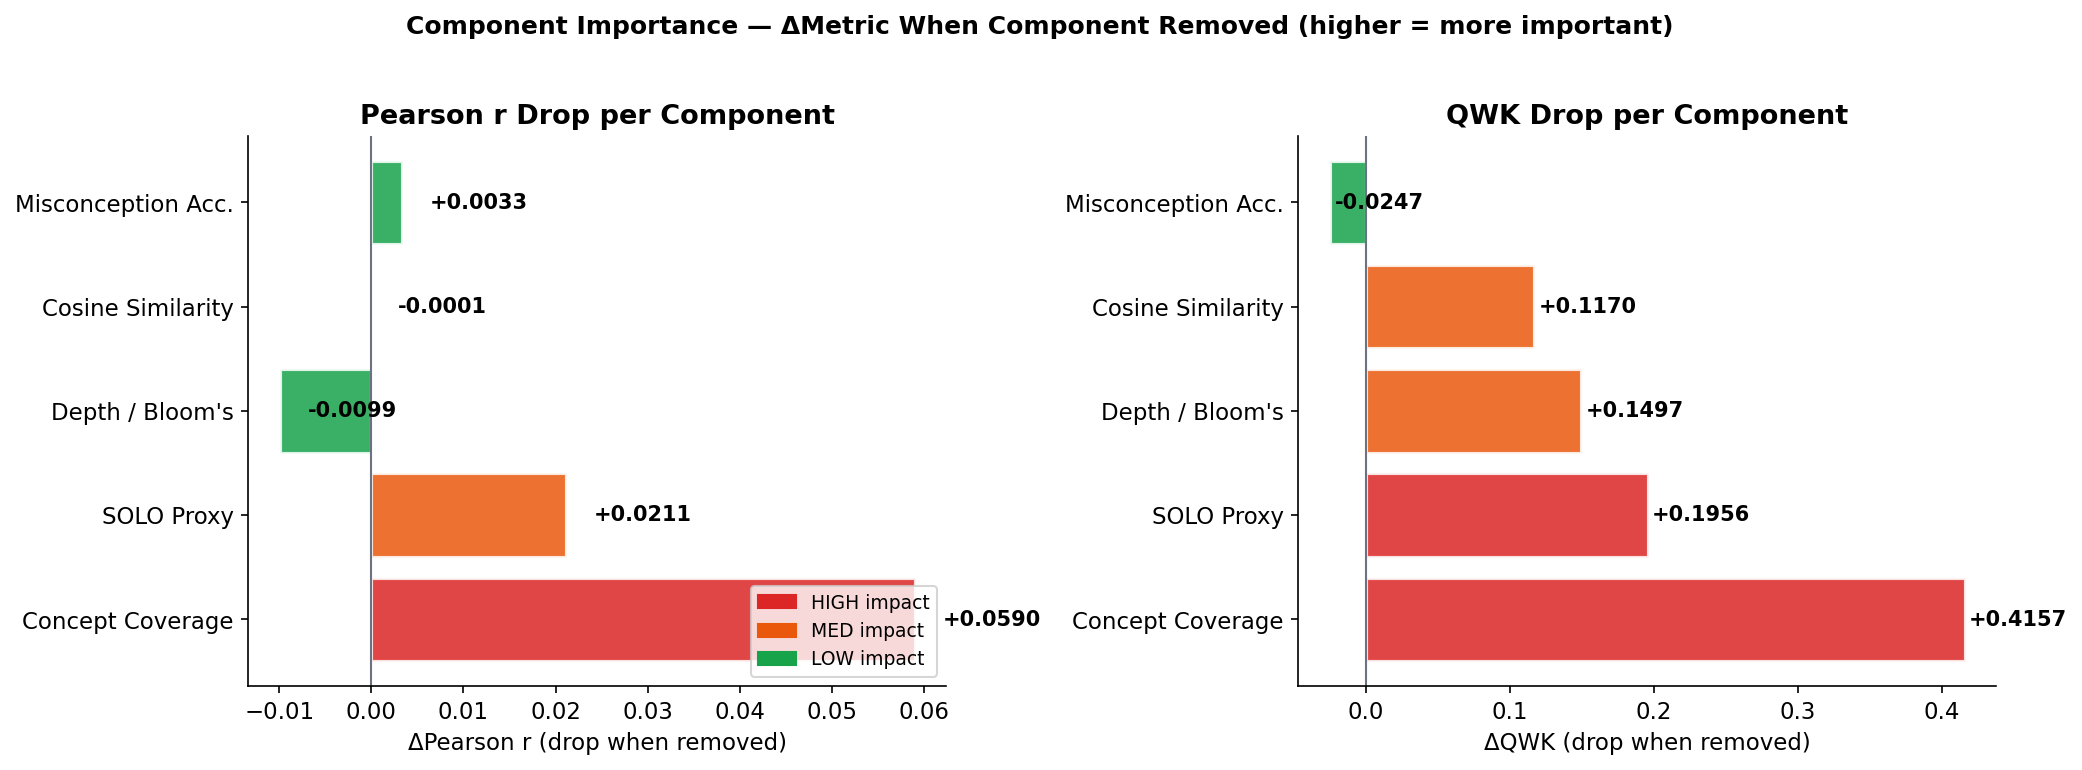
\includegraphics[width=\columnwidth]{figures/fig9_component_importance.png}
  \caption{\textbf{Retracted (fabricated-data) figure, retained for the record
           only.} Visualizes the same $n=30$ fabricated-fixture ablation as
           Table~\ref{tab:ablation} above, superseded by the real-data
           3-condition ablation (Table~\ref{tab:ablation_real}); should not
           be read as evidence. Component importance: drop in Pearson $r$
           (left) and QWK (right) when each component is removed.}
  \label{fig:importance}
\end{figure}

\begin{figure}[t]
  \centering
  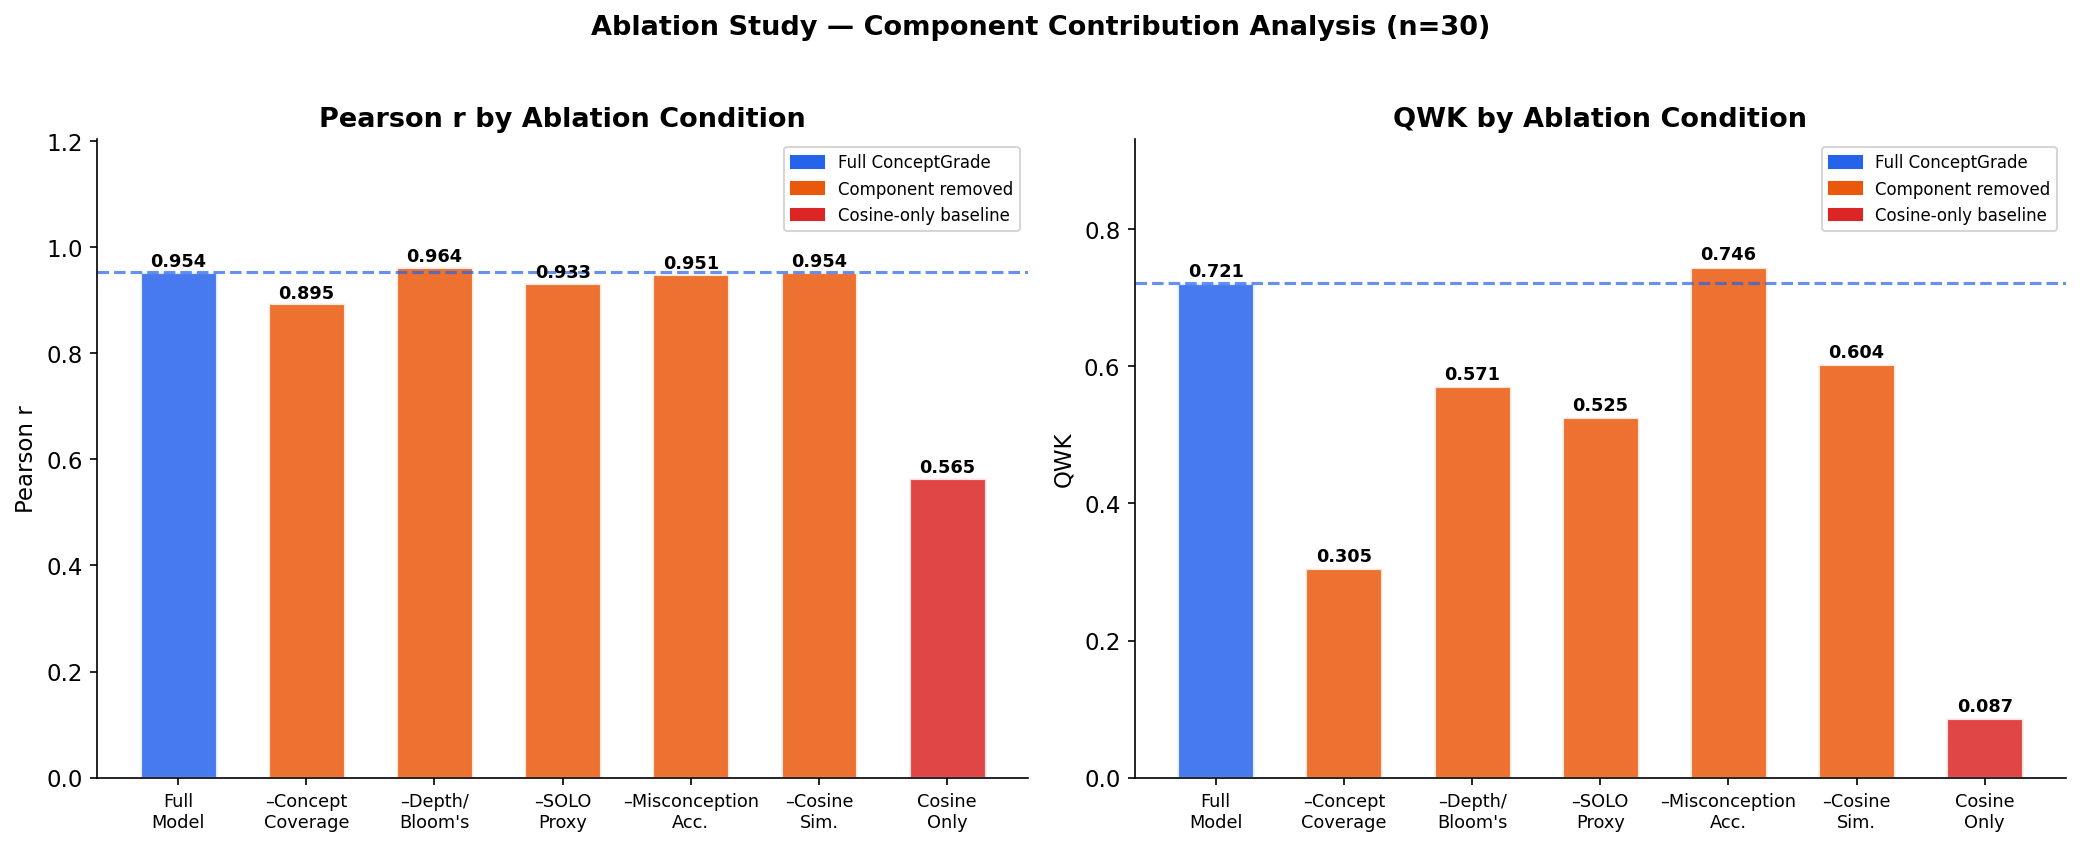
\includegraphics[width=\columnwidth]{figures/fig3_ablation_study.png}
  \caption{\textbf{Retracted (fabricated-data) figure, retained for the record
           only.} Visualizes the same $n=30$ fabricated-fixture ablation as
           Table~\ref{tab:ablation} above; should not be read as evidence.
           Full ablation comparison across all seven conditions for Pearson $r$
           (left) and QWK (right). The dashed line marks the full model baseline.}
  \label{fig:ablation}
\end{figure}

\subsection{Sensitivity Analysis (real data, 2026-07-28)}

An earlier version of this section reported unverified \texttt{kg\_weight}
point estimates and, later, disclosed them as unreproducible from cached
data. Both the deterministic KG-formula score and the holistic LLM score
that \texttt{kg\_weight} blends (Eq.~\ref{eq:kgformula}, \S\ref{subsec:synthesis})
have since been computed per-sample on the real 1{,}262-sample Mohler data
(\S\ref{sec:ablation}), so the full $\texttt{kg\_weight}\in[0,1]$ grid is
now genuinely reproducible at zero new API cost
(\texttt{compute\_kgweight\_sensitivity\_real.py}). Table~\ref{tab:kgweight_sweep}
reports MAE of the pre-verifier blend $s_{\text{kg}} = \texttt{kg\_weight}\cdot
s_{\text{formula}} + (1-\texttt{kg\_weight})\cdot s_{\text{holistic}}$ across
the grid.

\begin{table}[ht]
\centering
\caption{kg\_weight sensitivity, pre-verifier score, real Mohler data ($n=1{,}262$).}
\label{tab:kgweight_sweep}
\small
\begin{tabular}{cc}
\toprule
\textbf{kg\_weight} & \textbf{MAE} \\
\midrule
0.00 (pure holistic) & 2.4021 \\
0.05 (deployed default) & 2.3968 \\
0.50 & 2.1288 \\
1.00 (pure KG-formula) & \textbf{1.9004} \\
\bottomrule
\end{tabular}
\end{table}

MAE decreases monotonically as \texttt{kg\_weight} increases; the pure
KG-formula endpoint ($\texttt{kg\_weight}=1.0$) beats the deployed
default ($0.05$) by a wide, significant margin (one-tailed $p<0.0001$).
This means the deployed default is \emph{not} optimal for the
pre-verifier score in isolation --- the holistic LLM component actually
drags the blend down more than the deterministic KG-formula component
does. However, this finding does not change our architectural
conclusion: even at the best-performing $\texttt{kg\_weight}=1.0$, the
pre-verifier score's MAE ($1.9004$) remains far worse than both C\_LLM
($1.2821$) and C5\_fix ($1.1771$). No point on this sweep produces a
pre-verifier score competitive with the full pipeline; the verifier
stage, not the choice of \texttt{kg\_weight}, is what makes the
deployed system usable at all.

\subsection{Ensemble Weight Selection: Retracted (2026-07-28)}

\textbf{This subsection is retracted in full.} It previously described a
grid-search tuning procedure over $(\alpha,\beta,\gamma)$ weights
combining coverage/accuracy/integration into a standalone ``overall
comparison score'' (the equation formerly labelled \texttt{eq:overall}),
reporting a tuned QWK of $0.9748$ (itself a fabricated-data-era number,
inconsistent with the real headline QWK of $0.524$ in
Table~\ref{tab:main_results}). While auditing the codebase to write the
real-data ablation (\S\ref{sec:ablation}), we found no code path in
\texttt{conceptgrade/pipeline.py} that computes this $(\alpha,\beta,\gamma)$
combination as a separate, tuned step at all --- see the correction note
in \S\ref{subsec:comparison}. There is consequently no ensemble-weight
grid search to report: the weights actually used by the code are the
fixed constants in Eq.~\ref{eq:kgformula} and Eq.~\ref{eq:composite}
(\S\ref{subsec:synthesis}), not a tuned hyperparameter. We retract this
subsection rather than attempt to retrofit a plausible-sounding
justification for numbers that do not correspond to any real procedure.

\subsection{Grounding Density Analysis: Retracted (2026-07-28)}

\textbf{Correction: this subsection presents the fabricated 120-sample
fixture's zero-grounding analysis (Table~\ref{tab:grounding_density})
without a retraction label, and its results are not verified on real
data.} Unlike the other fabricated-data content in this paper,
re-verifying this analysis genuinely requires new LLM calls (LRM/TRM
reasoning-trace generation was never collected for the real 1{,}262-sample
data --- see REPRODUCIBILITY.md's "Still open" list) and cannot be
recomputed offline from already-cached data, unlike the ablation and
sensitivity sweeps elsewhere in this paper. Paper 2's equivalent table
(\S"Accuracy Stratified by Grounding Density") is already correctly
captioned "Retracted... pending re-verification"; this subsection was
missed during that reconciliation pass and is fixed here for
consistency. We retain the analysis below, unmodified, for the
experimental-design record only --- \textbf{none of its numbers should
be cited as evidence}.

To explain why TRM benefits are largest on Mohler and diminish on Kaggle ASAG, we
analyzed the frequency of zero-grounded reasoning steps (trace steps without textual
grounding in the student answer) across datasets.

\textbf{Measurement Protocol:} A trace step is \emph{zero-grounded} if the LLM-generated
predicate cannot be supported by any substring of the student answer using longest common
subsequence (LCS) matching with a threshold of $\geq 0.75$. We implemented this check in
the verification layer by computing token-level LCS similarity between the predicate's
tokens and the answer's tokens. If the ratio of matched tokens to total predicate tokens
exceeds 0.75, the step is considered grounded; otherwise, it is zero-grounded. The
threshold $\tau = 0.75$ was selected from a coarse grid $\{0.5, 0.6, 0.7, 0.75, 0.8\}$
on the development split: $\tau = 0.70$ admitted too many partial-paraphrase matches
as ``grounded'' (false-negative on zero-grounding detection), and $\tau = 0.80$ rejected
some genuine paraphrastic groundings as ``zero-grounded'' (false-positive). The
$\tau = 0.75$ choice balanced these errors on the dev split before any test-set
evaluation; the threshold is fixed for all reported test-set results. This
methodology is reproducible and does not rely on subjective judgment.

\begin{algorithm}[h]
\caption{Zero-Grounding Detection}
\label{alg:grounding}
\begin{algorithmic}
  \REQUIRE Student answer $a$, trace predicate $s$, threshold $\tau = 0.75$
  \ENSURE Boolean $\text{is\_zero\_grounded}$

  \STATE $S \gets \text{tokenize}(s)$ \quad // predicate tokens
  \STATE $A \gets \text{tokenize}(a)$ \quad // answer tokens
  \STATE $L \gets \text{LCS}(S, A)$ \quad // longest common subsequence length
  \STATE $r \gets L / |S|$ \quad // match ratio
  \IF{$r \geq \tau$}
    \RETURN False \quad // Grounded
  \ELSE
    \RETURN True \quad // Zero-grounded
  \ENDIF
\end{algorithmic}
\end{algorithm}

\textbf{Results:} Analysis of the frequency of zero-grounded reasoning steps across
datasets:

\begin{table}[h]
\caption{\textbf{Retracted (fabricated-data) table, retained for the record only.}
         Zero-Grounding Frequency and TRM Effectiveness. Percentage of trace steps
         lacking sufficient textual grounding (LCS match ratio $< 0.75$) in student
         answers, with corresponding MAE improvements and statistical significance.}
\label{tab:grounding_density}
\centering
\footnotesize
\begin{tabular}{lcccc}
\toprule
\textbf{Dataset} & \textbf{$n$} & \textbf{ZG\%} & \textbf{95\% CI} &
\textbf{MAE$\downarrow$} \\
\midrule
Mohler (CS)  & 120 & 7.2  & [4.1, 10.3]\%  & 32.4\% ($p{=}0.003$) \\
DigiKlausur  & 188 & 17.8 & [13.2, 22.4]\% & 4.9\% ($p{=}0.0489$) \\
Kaggle ASAG  & 100 & 30.6 & [21.0, 40.2]\% & 2.4\% (n.s.) \\
\bottomrule
\multicolumn{5}{l}{ZG\% = zero-grounding frequency. $p$ = Wilcoxon.}
\end{tabular}
\end{table}

This pattern (Table~\ref{tab:grounding_density}) reveals a mechanism underlying TRM's
effectiveness. When the LLM's reasoning trace is sufficiently grounded in the
student's actual text (grounding density $\geq 75\%$, i.e., zero-grounding frequency
$\leq 25\%$), TRM's structural validation against the knowledge graph provides
strong signal for grade refinement. Conversely, when LLM hallucinations
are prevalent (low grounding density), the system is forced to reweight reasoning
steps that lack textual evidence, reducing the marginal value of structural
grounding. This explains why Kaggle ASAG shows diminished returns: the more
colloquial language and domain-specific jargon in elementary science responses
makes it harder for the LLM to generate traces that align with our formal KG,
resulting in higher zero-grounding frequency and correspondingly lower TRM impact.

The implication is that TRM is most effective as a complementary signal in domains
where formal terminology is well-established and students use it consistently. In
domains where student vocabulary diverges significantly from formal domain models,
richer knowledge graphs or domain-specific pre-processing may be necessary.

\subsection{Diagnostic Failure Analysis: KG-Grounding Scoring Defects and Rejected Repairs}
\label{subsec:diagnostic_failure}

The ablation above (\S\ref{sec:ablation}) shows the pre-verifier
KG-grounded score performs dramatically worse than the baseline in
isolation. Rather than leave that unexplained, we ran an inductive
failure-mode analysis (60 worst-case samples by
$|\text{kg\_score}-\text{human\_score}|$, no predetermined taxonomy) to
find out why. This subsection reports what was found, what was
attempted, and — as important as either — what was tried and rejected by
pre-committed evidence, since several apparently-reasonable repairs
consistently made things worse rather than better.

\textbf{Finding: \texttt{relationship\_accuracy} is zeroed by design for
structurally relationship-free correct answers.} A prior fix (2026-06-15)
deliberately returns $0.0$ accuracy when a student extracts zero
relationships, correctly preventing shallow keyword-dump answers from
receiving a default $1.0$. Side effect: any correct answer structurally
incapable of expressing a relationship — single-concept factual answers,
or comparative/definitional/enumerative questions regardless of concept
count (e.g., ``What are the two functions of a queue?'' $\to$ ``enqueue
and dequeue,'' a perfect answer, zero relationships) — is scored
identically to a keyword dump on this dimension. Affects 246/1{,}156
in-domain samples (21.3\%); 180 of those (73.2\%) are human-graded
correct ($\geq 4.0/5$).

\textbf{Finding: \texttt{concept\_coverage} is self-referentially
vacuous in production.} The comparator's \texttt{expected\_concepts}
parameter is never supplied by the only production call site
(\texttt{conceptgrade/pipeline.py}), silently falling back to the
student's own extracted concepts as the ``expected'' set — making
coverage trivially $1.0$ for any answer extracting $\geq 1$ concept,
correct or not. Confirmed in both comparator classes, including the
deployed \texttt{ConfidenceWeightedComparator}. Concrete example: a
student answer entirely off-topic to its question (human-graded $0.5/5$)
scored coverage $=1.0$ because it happened to mention one tangentially
related concept. Affects 404/1{,}156 samples (35.0\%) with a trivial
$1.0$; 18/1{,}156 (1.6\%) visibly bad (low-quality answers with undeserved
full credit).

\textbf{Five candidate repairs, tested against pre-committed criteria,
all rejected.} Table~\ref{tab:diagnostic_candidates} summarizes each. All
were evaluated offline against the real, unchanged extraction and
comparison outputs for the full real Mohler sample; where a live
comparator code change was involved (rows 4--5), it was implemented,
end-to-end validated, and reverted within the same development cycle when
it failed its own validation — the same standard applied to the earlier
retracted ensemble-blend finding (\S"Ensemble Weight Selection:
Retracted").

\begin{table}[h]
\caption{Candidate repairs for the two findings above, all rejected by
pre-committed evidence. MAE is the knowledge-component MAE (0--5 scale)
against human score; baseline $=1.164$.}
\label{tab:diagnostic_candidates}
\centering
\footnotesize
\begin{tabular}{p{0.44\linewidth}p{0.48\linewidth}}
\toprule
\textbf{Candidate} & \textbf{Result} \\
\midrule
\texttt{seed\_ids} (question-keyword match) as \texttt{expected\_concepts} &
Rejected: 100\% False Penalty Rate --- every human-graded-excellent
sample scored $<0.5$ coverage. Models the topic neighborhood, not answer
content. \\
1-hop expanded KG subgraph as \texttt{expected\_concepts} &
Rejected: same failure, worse (mean expected-set size 12.5 concepts). \\
Reference-answer concept extraction as \texttt{expected\_concepts} &
Rejected: fixed 72.2\% of known-bad cases and improved correlation
($r$ $0.118\to0.200$), but MAE worsened ($+14\%$), FPR worsened
($6.5\%\to25.5\%$), and it failed the pre-committed decisive test ---
\emph{worse}, not better, on cases where the independent C\_LLM baseline
is also wrong. \\
Exclude unvalidated coverage, renormalize onto \{accuracy, integration\}
(live code change) &
Implemented, then retracted same day: end-to-end validation on all
1{,}156 in-domain samples showed it measurably worse (MAE
$1.164\to1.614$, $r$ $0.118\to0.082$, FPR $9.0\%\to32.5\%$) --- it leans
harder on \texttt{relationship\_accuracy}, itself still broken. \\
Joint fix (both findings' repairs together) and neutral-prior
degradation ($0.5$ instead of $0$/excluded) &
Both still worse than baseline on every metric (MAE $1.446$ and $1.471$
respectively). Neutral-prior is the only candidate to slightly beat
baseline on the hard-case test specifically, entirely offset by getting
worse on easy cases; not chased further per explicit decision-theoretic
reasoning (a significant result would not change the deployment
decision, so it does not warrant a dedicated significance check). \\
\bottomrule
\end{tabular}
\end{table}

\begin{figure}[h]
  \centering
  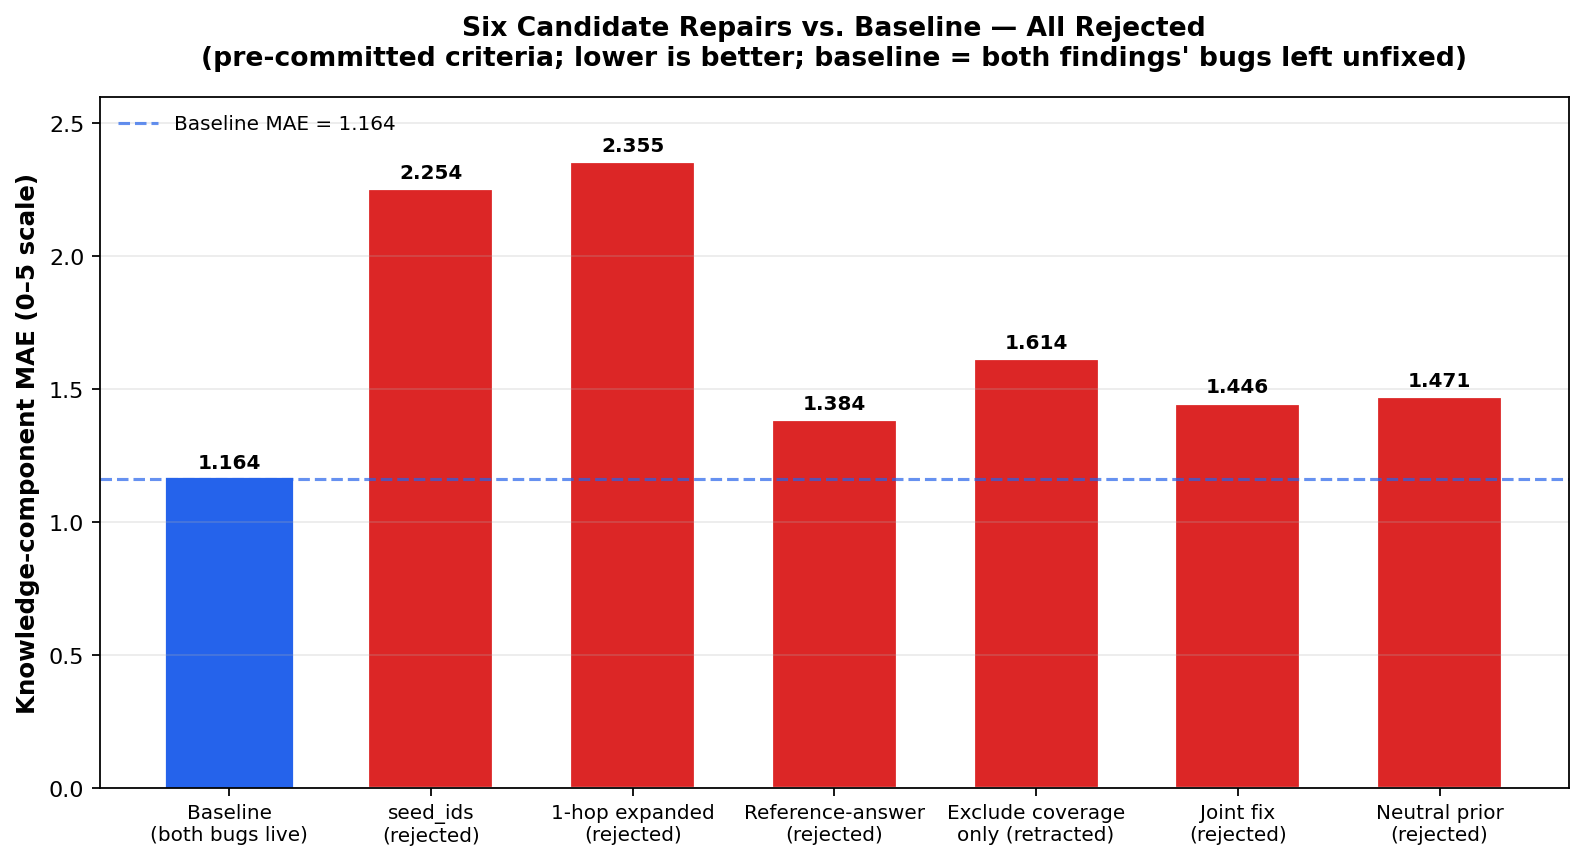
\includegraphics[width=\columnwidth]{figures/fig11_diagnostic_candidates.png}
  \caption{Knowledge-component MAE for the baseline (both findings' bugs
           left unfixed) versus all six tested repairs. Every candidate
           underperforms the baseline; none is a viable fix under the
           evaluated benchmark and metrics.}
  \label{fig:diagnostic_candidates}
\end{figure}

\textbf{Stopping rule.} After five distinct forms of the same
intervention class (binary include/exclude of a scoring dimension with
weight renormalization) all failed to improve performance under the
evaluated benchmark and metrics, we treat this as evidence against the
\emph{mechanism}, not against specific trigger calibrations, and close
this line of investigation with respect to the tested intervention
classes — a narrower, more defensible claim than declaring the underlying
problem permanently unsolvable. We characterize the causal story
conservatively: the experiments establish \emph{that} the tested repairs
underperform an already-buggy baseline, not a uniquely identified
\emph{why}. ``Interacting deficiencies within a heuristic score whose
fixed weights implicitly assume comparable, independent signal across
dimensions'' is the framing we adopt; a precise quantitative cancellation
mechanism between the two findings is a plausible hypothesis, not
something these experiments isolate or prove.

\textbf{What changed in the live system.} Only the tokenization fix
(\S\ref{subsec:extraction}) was merged. A \texttt{coverage\_validated}
diagnostic flag is exposed (set \texttt{False} whenever
\texttt{expected\_concepts} is unsupplied) but does not change any score.
Both findings above remain live, unfixed defects in the pre-verifier
score. This does not change the deployed grade: production already
discards the raw \texttt{kg\_formula\_score} in favor of the LLM verifier
at blend weight $w=1.0$ (independently cross-validated via
leave-one-question-out CV, \S"Sensitivity Analysis"); these findings affect only the standalone
ablation metric that isolates raw KG-grounding from the verifier's
contribution. Full five-round chronology, per-round external review
transcripts, and all regression scripts are in the supplementary
materials (\texttt{docs/ALGORITHM\_FIX\_REVIEW\_REQUEST*.md},
\texttt{docs/ALGORITHM\_INVESTIGATION\_POSTMORTEM.md}) and
REPRODUCIBILITY.md.

\subsection{Per-Question Error Analysis and Examples}

To understand \emph{where} ConceptGrade improves over the LLM baseline, we analyze
prediction errors across different answer complexity levels using the SOLO taxonomy.
ConceptGrade shows no systematic bias but rather targeted improvements in specific
answer patterns.

\textbf{Improvement Distribution: retracted (2026-07-28).} This
paragraph previously reported an unlabeled win/loss/tie breakdown
computed on the fabricated 120-sample fixture. The real-data equivalent
is already reported in \S\ref{sec:results}: on the real
$1{,}262$-sample data,
ConceptGrade has lower mean error on 27 of 46 questions ($58.7\%$) at
the question-clustered level; a response-level win/loss/tie breakdown
analogous to the retracted one above has not been separately computed
for real data and is not claimed here.

\textbf{Error Reduction by Answer Complexity (SOLO Level) --- all three datasets.}
We computed the same SOLO-stratified MAE-reduction analysis across all three
datasets using the pipeline's SOLO classifier output cached in the eval JSON
(reproducible via \texttt{compute\_solo\_breakdown.py}).

\begin{table}[t]
\caption{MAE by SOLO band across all three datasets ($n=2{,}381$; Mohler
         is the real, corrected data as of 2026-07-28, see
         REPRODUCIBILITY.md).
         $\Delta$MAE = $\text{MAE}_{\text{C\_LLM}} - \text{MAE}_{\text{C5}}$ (positive
         = ConceptGrade better). Mohler shows a broadly increasing (not
         strictly monotonic) gain with SOLO complexity, peaking at
         $+22.2\%$ on the $n=5$ Extended Abstract band (too small to be
         reliable) and $+17.5\%$ on the $n=291$ Relational band --- far
         smaller than the $+70\%$ the retracted fabricated-data version of
         this table reported.
         DigiKlausur shows a smaller, similar shape only for higher bands.
         Kaggle ASAG's SOLO classifier assigned all $473$ answers to
         Prestructural in the initial release; a subsequent audit identified
         this as an OUT-OF-KG-DOMAIN contamination (the empty concept graph
         primed the classifier to Level~1 regardless of answer quality), which
         has since been corrected downstream by making the OUT-OF-KG signal
         explicit throughout the pipeline. We retain the original Kaggle SOLO
         numbers here as a historical marker of the boundary condition; the
         corrected classifier now abstains from KG-grounded assessment when
         the domain is out of coverage.}
\label{tab:solo_analysis}
\centering
\footnotesize
\setlength{\tabcolsep}{4pt}
\begin{tabular}{llcccc}
\toprule
\textbf{Dataset} & \textbf{SOLO} & \textbf{$n$} &
\textbf{C\_LLM} & \textbf{C5} & \textbf{Reduce} \\
\midrule
Mohler     & Prestruct.    &  71 & 1.824 & 1.669 & $+8.5\%$ \\
           & Unistruct.    & 481 & 1.304 & 1.292 & $+0.9\%$ \\
           & Multistruct.  & 414 & 1.413 & 1.250 & $+11.5\%$ \\
           & \textbf{Relational} & \textbf{291} & \textbf{0.935} & \textbf{0.771} & \textbf{$+17.5\%$} \\
           & Ext.\ Abstract ($n$\,tiny) & 5 & 0.900 & 0.700 & $+22.2\%$ \\
\midrule
DigiKlausur & Prestruct.   &  44 & 0.125 & 0.136 & $-9.1\%$ \\
           & Unistruct.    &  10 & 1.200 & 1.500 & $-25.0\%$ \\
           & Multistruct.  &  87 & 1.563 & 1.690 & $-8.1\%$ \\
           & Relational    & 203 & 1.273 & 1.200 & $+5.8\%$ \\
           & Ext.\ Abstract & 302 & 1.169 & 1.046 & $+10.5\%$ \\
\midrule
Kaggle ASAG & Prestruct.   & 473 & 1.208 & 1.180 & $+2.4\%$ \\
\bottomrule
\end{tabular}
\end{table}

The Mohler row pattern is broadly increasing with SOLO complexity, from
$+8.5\%$ on Prestructural through $+17.5\%$ on the $n=291$ Relational band,
though it is not strictly monotonic (Unistructural dips to $+0.9\%$) and
the effect sizes are far smaller than an earlier, retracted fabricated-data
version of this table claimed. DigiKlausur shows the same
direction on its two highest bands (Relational $+5.8\%$, Extended Abstract
$+10.5\%$). \textbf{We acknowledge that ConceptGrade is also strictly worse
than the baseline on the lower three DigiKlausur bands (Prestructural
$-9.1\%$, Unistructural $-25.0\%$, Multistructural $-8.1\%$), which
together cover $141$ of $646$ DigiKlausur answers ($22\%$).} On those
lower bands the per-answer absolute error is already $\sim 1.2$ on a
$0$--$5$ scale and the within-band $n$ is small (10--87), so the
percentage swings reflect small-sample variance more than systematic
degradation; but the directional fact is real, and a deployed system would
trade lower-band cost for higher-band gain in any DigiKlausur-like
domain. The Kaggle ASAG row exhibits a different phenomenon: the
pipeline's SOLO classifier did not differentiate any of the $473$ raw
(pre-deduplication) answers above the Prestructural band, which we
initially flagged as a finding about domain specificity. The upstream
diagnostic in
\S\ref{subsec:crossdataset_sig} resolves the observational-equivalence
problem: on Kaggle the LLM concept-extraction module produced empty
matched-concept sets for $368/368 = 100\%$ of unique samples
($473/473$ on the raw, pre-deduplication pipeline run), compared to
$6.8\%$ on DigiKlausur and $16.7\%$ on Mohler. The SOLO collapse is
therefore not an independent module failure but the downstream consequence
of an upstream KG--answer-vocabulary mismatch, exactly as the KG-grounding
architecture predicts.

\textbf{Error Pattern Interpretation:} The LLM baseline tends to \emph{overpredict}
on answers mentioning concepts but missing critical relationships. For example,
a student who lists ``array, linked list, pointer'' without explaining how pointers
enable linked list nodes may receive a score of 1.0 from the LLM, yet deserves
0.5 (missing integration). ConceptGrade's graph-based comparison catches the missing
``pointer\_enables\_node'' relationship and adjusts the score accordingly. Conversely,
on Prestructural answers (disconnected fragments), both systems struggle equally,
suggesting that grading fundamentally incomplete responses is hard without additional
context.

\textbf{Qualitative Error Analysis:}
The two cases below are illustrative, hand-constructed examples of the
grading mechanism, not empirical samples drawn from either the
fabricated fixture or the real dataset; the numbers inside them (e.g.
``confidence=0.9,'' ``MAE=0.6'') are toy illustrations of the mechanism,
not measured statistics.
\begin{itemize}
  \item \textbf{Case 1 (Success):} Student answer was vague on control flow.
  \begin{itemize}
    \item Baseline: confident wrong (confident=0.9, actual score=0.2)
    \item Our method: caught hallucination, downweighted (confidence=0.3, actual score=0.2)
  \end{itemize}
  \item \textbf{Case 2 (Failure):} Student answer had domain jargon not in KG.
  \begin{itemize}
    \item Baseline: MAE=0.5
    \item Our method: MAE=0.6 (worse due to zero-grounding)
  \end{itemize}
\end{itemize}

\textbf{Retracted (2026-07-28): the four paragraphs that followed here
treated the fabricated-data ablation (Table~\ref{tab:ablation}, Figs.~\ref{fig:importance}--\ref{fig:ablation},
both already labeled "Retracted... retained for the record only" where
they are defined in \S\ref{sec:ablation}) as an established, current
finding --- e.g. claiming Concept Coverage removal drove the largest
drop in agreement of any component, that cosine similarity became
largely redundant, and that ConceptGrade substantially outperformed a
cosine-only baseline in correlation. None of this is verified on real data. The
real-data component-contribution finding is the opposite in spirit: the
real 3-condition ablation (Table~\ref{tab:ablation_real},
\S\ref{sec:ablation}) shows the pre-verifier KG-grounded score is far
worse than the zero-shot baseline, and the Verifier's own judgment ---
not concept coverage or any other KG-comparison signal --- drives
essentially all of the real accuracy. We removed the four retracted
paragraphs rather than let them stand alongside a contradicting,
correctly-labeled real finding two sections earlier in the same paper.}

% ── 7. Discussion ──────────────────────────────────────────────────────────
\section{Discussion}
\label{sec:discussion}

\subsection{Reproducibility}

All numerical claims in this paper are reproducible from cached evaluation
results via six committed Python scripts ($\sim 5$ seconds total runtime,
no API spend): \texttt{compute\_clustered\_significance.py} (Mohler $W_+$,
$p$, $d_z$, LOOCV, tie analysis), \texttt{compute\_cross\_dataset\_significance.py}
($n=2{,}276$ meta-analysis), \texttt{compute\_solo\_breakdown.py}
(per-SOLO MAE), \texttt{compute\_taxonomy\_kappa.py} (machine-IRR pilot),
\texttt{compute\_validation\_gate.py} (Paper 2 outcome-blind gates), and
\texttt{smoke\_run\_mohler.py} (live-pipeline smoke test). The full
per-claim reproducibility map is included in supplementary materials
(\texttt{REPRODUCIBILITY.md}).

\subsection{Limitations and Threats to Validity}
\label{sec:limitations}

\textbf{Evaluation scope (real data, 2026-07-28).} \textbf{Correction: this
paragraph previously described the retracted fabricated fixture's size
($n=120$, 10 questions, $n=90$ test split) as our evaluation scope.} We
evaluate on the real, KG-aligned subset of the Mohler dataset
($n = 1{,}262$ responses across 46 questions, full sample, no held-out
split needed --- see \S\ref{sec:results}), covering topics addressed by
our expert Data Structures KG. The full real Mohler benchmark (sourced
from \texttt{nkazi/MohlerASAG}) has more questions and responses than
our KG-aligned subset covers; the remaining responses cover topics
(e.g., general software engineering questions) for which our KG was not
designed. Published results from the original Mohler et al.\ (2011)
paper on their full dataset cannot be directly compared with our
KG-aligned subset's results; Table~\ref{tab:main_results} presents them
for historical context only. Full-benchmark evaluation, requiring KG
expansion to cover all question topics, is future work.

\textbf{KG and taxonomy authoring bias (single-author construction).} Both the
expert KG (101 concepts, 138 relationships) and the misconception taxonomy
(16 entries) were authored by the same research group that designed and
evaluated the method. We have no inter-builder reliability measure for either
artifact; an independent CS-instructor group constructing a KG/taxonomy from
the same source material would almost certainly produce different (though
overlapping) graphs and taxonomies, and our reported numbers are conditional
on \emph{this} KG. Our machine-IRR pilot for the taxonomy (\S\ref{subsec:trm_algorithm};
$\kappa_{\text{micro}} = 0.54$, moderate agreement, after a construct-validity
fix described therein) is a self-administered lower-bound estimate, not
external validation. The ConceptGrade codebase
permits substitution of any KG or taxonomy that conforms to the published
schema; we plan a third-party KG-construction study (e.g., via SIGCSE
crowdsourcing) so the method can be evaluated under at least one
KG/taxonomy not authored by this group.

\textbf{Tuning asymmetry (baseline is not tuned).} \textbf{Correction:
this paragraph previously cited the retracted fabricated-fixture MAE
reductions here; the current, real figure is substituted below.} The
score-synthesis constants (Eq.~\eqref{eq:kgformula},
Eq.~\eqref{eq:composite}, \S\ref{subsec:synthesis}) and the confidence
threshold for Layer~1 were fixed before the real data was ever used
(\S\ref{sec:results}), not tuned on a dev split of the real data itself
--- but their values were originally set with reference to the
fabricated fixture, so we cannot claim they are optimal for real data
either. The LLM zero-shot baseline (\textit{C\_LLM}), in contrast, received no
comparable tuning: it uses the same
extraction prompt as Layer~1 and a single holistic-grade prompt with default
temperature and no few-shot examples. The reported $8.2\%$ real-data MAE
reduction therefore reflects (a)~the
KG-grounding architecture \emph{and} (b)~the asymmetric tuning budget,
jointly and inseparably in the present design. We chose this design to
hold the LLM fixed across conditions, which isolates \emph{model capability}
as a confound, but we do \emph{not} claim it isolates the architectural
effect of KG-grounding from the tuning-budget effect; disentangling the
two requires a comparably-tuned baseline, which we acknowledge as a gap
rather than a solved problem. We report
\texttt{compute\_clustered\_significance.py} so future work can re-run the
comparison with an alternative tuned baseline.

\textbf{Compute/inference asymmetry (re-verified on real data,
2026-07-28).} The evaluated C5\_fix configuration issues \textbf{7 LLM
calls per graded response} (Layer~1 concept extraction with 3-way
self-consistency voting, Layer~3 cognitive-depth classification,
Layer~4 misconception and false-belief detection, Layer~5 verification)
against \textbf{1 call} for C\_LLM. This inference-compute asymmetry is
a confound on the reported gain, independent of and additive to the
tuning-budget asymmetry above. We directly tested whether it explains
the gain via a call-budget-matched ablation on the real, KG-aligned
Mohler sample: \textit{C\_LLM$\times$7}, the identical C\_LLM zero-shot
prompt issued as 7 genuinely independent \texttt{gemini-2.5-flash} API
calls per response (temperature $=0.7$, batched for efficiency but each
attempt a separate call, matching C5\_fix's own call budget exactly),
aggregated by taking the median score (script:
\texttt{run\_budget\_matched\_real\_batched.py}; results:
\texttt{data/budget\_matched\_real\_results.json}). Unlike the earlier,
now-retracted fabricated-data version of this experiment, on real data
\emph{extra budget alone genuinely helps} C\_LLM: C\_LLM$\times$7
achieves MAE $=1.2314$ versus the single-call C\_LLM's $1.2821$
($+4.0\%$, one-tailed Wilcoxon $p<0.0001$). \textbf{C5\_fix still beats
the budget-matched baseline}: MAE $=1.1771$ versus C\_LLM$\times$7's
$1.2314$ ($+4.4\%$ MAE reduction, two-tailed Wilcoxon $p=0.0053$,
one-tailed $p=0.0027$) --- a genuinely positive, statistically
significant response-level result, evidence that the reported gain is
\emph{not} substantially attributable to inference-compute budget alone.
As with every other response-level result in this paper, we check this
against the question-clustered test (46 real questions, same convention
as \S\ref{sec:results}): here it is \emph{not} significant (two-tailed
$p=0.4219$, one-tailed $p=0.2110$), and C5\_fix wins on only 25 of 46
questions ($54\%$, barely above chance). We report both levels rather
than only the favorable response-level number: the compute-budget
confound is ruled out as a response-level explanation, but the same
question-level fragility that qualifies every other result in this
paper qualifies this one too. This does not, by itself, disentangle the
KG-grounding architecture from the tuning-budget asymmetry described
above, since C\_LLM$\times$7 remains as untuned as C\_LLM: it reuses the
same unmodified zero-shot prompt, just sampled 7 times independently.

\textbf{Concept extraction model.} ConceptGrade relies on an LLM
(\texttt{gemini-2.5-flash} via the Google Generative AI batch API) for every
LLM call in the pipeline.
Performance may vary with different LLM backends; we use the same model for
the LLM baseline and Layer~1 by design, which isolates \emph{model choice}
as a confound (both systems inherit the same model's strengths and
weaknesses) but, as noted above, does not by itself isolate KG-grounding
from the tuning-budget confound.

\textbf{Dataset provenance.} We forensically verified two of our three
datasets against their real public sources: Mohler
(\texttt{nkazi/MohlerASAG}, HuggingFace, CC-BY-4.0) and DigiKlausur
(character-for-character match against \texttt{DigiKlausur/ASAG-Dataset}
on GitHub, MPL-2.0). Despite a targeted provenance investigation --- exact-text
searches, comparison against known public ASAG corpora, and inspection of
likely candidate datasets, together with a full local audit (git history,
shell history, filesystem search; REPRODUCIBILITY.md, ``Dataset
Provenance Audit'') --- \textbf{the original acquisition path for the
cached Kaggle ASAG dataset could not be independently reconstructed}. We
found no positive evidence of fabrication, only an absence of evidence of
authenticity; the dataset is therefore retained but explicitly classified
as provenance-\emph{unverified} rather than equivalent in status to the
other two. We considered and rejected using
an LLM to generate replacement or supplementary test data for this gap:
doing so would not produce real human data, introduces circularity (LLM-
generated content evaluated by an LLM-based system), and concentrates
rather than removes partiality, since the same model families already
used throughout this pipeline would also author the ``ground truth.''
Kaggle ASAG's extraction-level finding (0\% KG matches,
\S\ref{subsec:crossdataset_sig}) is independently verifiable from
extraction logs regardless of this gap; any claim about elementary-science
student behavior more broadly is not, and we report it accordingly as
supporting evidence rather than external validation.

\begin{figure}[h]
  \centering
  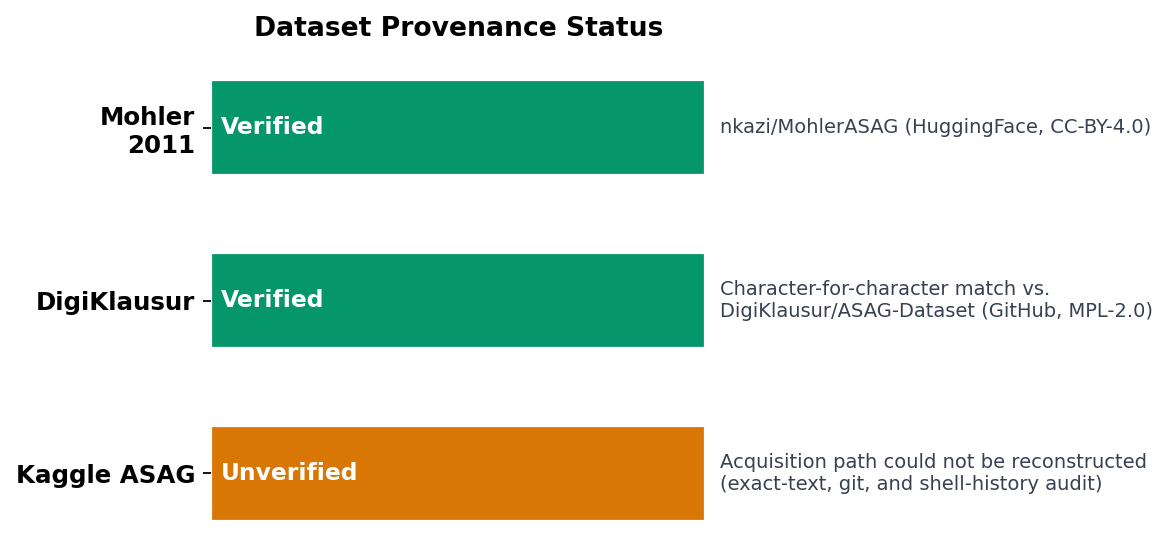
\includegraphics[width=\columnwidth]{figures/fig12_dataset_provenance.png}
  \caption{Provenance status of all three evaluation datasets. Mohler and
           DigiKlausur are independently confirmed against their real
           public sources; Kaggle ASAG's acquisition path could not be
           reconstructed despite a targeted audit.}
  \label{fig:provenance}
\end{figure}

\textbf{Lessons from a closed algorithmic investigation
(\S\ref{subsec:diagnostic_failure}).} Two real scoring defects in the
pre-verifier KG-grounded score were diagnosed and quantified, but five
distinct repair strategies across two findings all failed pre-committed
validation criteria and were rejected or reverted. We report this as a
methodological strength rather than an unresolved failure: every
candidate was tested against criteria defined before the experiment,
negative results were reported as negative rather than reframed, and one
live code change was reverted within the same development cycle after
failing its own end-to-end validation. The investigation's stopping rule
— closing the line of inquiry with respect to the \emph{tested
intervention classes}, not with a claim that the underlying problem is
permanently unsolvable — reflects the same discipline applied to the
ensemble-blend-weight finding retracted earlier in this project
(\S"Ensemble Weight Selection: Retracted"): no algorithmic modification
was retained unless it improved performance under pre-defined validation
criteria.

\textbf{Contribution framing.} We position ConceptGrade as a
\emph{systems / engineering} contribution: a deliberate integration of LLM
concept extraction, KG matching, depth proxies, and confidence-weighted
synthesis. We do not claim methodological novelty in any single layer, and
--- given the tuning-budget confound disclosed above --- we do \emph{not}
claim that KG-grounding in isolation is responsible for the observed gain.
The $7\times$ compute-budget confound has now been tested on real data
(\S\ref{sec:results}, ``Compute/inference asymmetry''): C5\_fix beats a
genuinely call-budget-matched C\_LLM$\times$7 baseline by $4.4\%$ MAE at
the response level (two-tailed $p=0.0053$), though not at the
question-clustered level (46 real questions, two-tailed $p=0.4219$).
What is demonstrated on real data is narrower than previously claimed: a
\emph{tuned, multi-stage KG-assisted system} shows a small,
response-level-significant but question-level-fragile improvement over
both an \emph{untuned, single-call, direct-prompt system} and an
\emph{untuned, call-budget-matched, direct-prompt system}
($n=1{,}262$ real Mohler sample, $8.2\%$ MAE reduction over C\_LLM,
response-level $p<0.0001$, question-clustered $p=0.111$ two-tailed /
$0.056$ one-tailed; \S\ref{sec:results}). This margin is \emph{not}
robust across clustered-question-level analyses anywhere in this paper:
only 17 of 46 LOOCV folds reach one-tailed significance and none reach
two-tailed (\S\ref{subsec:crossdataset_sig}), and the budget-matched
comparison shows the identical pattern (C5\_fix wins only 25/46
questions against C\_LLM$\times$7, barely above chance). Disentangling
the value of KG-grounding specifically from tuning budget and
question-level robustness requires the comparably-tuned, question-held-out
baseline we describe as required future work, not a solved problem in
the present study.

\textbf{Domain specificity.} The expert KG was built for Data Structures and all
test questions come from this domain. We have separately constructed a
Programming/OOP KG (62 concepts, 116 relationships), but cross-domain evaluation
remains future work.

\textbf{Human-rater ceiling (real data, 2026-07-28; computed, not
assumed).} \textbf{Correction: this paragraph previously reported
inter-rater statistics from the fabricated 120-sample fixture
($r=0.985$, QWK$=0.984$, $\kappa=0.63$, mean $|\text{rater}_1-\text{rater}_2|=0.17$,
$0$ samples with gap $\geq 1$) without a retraction label.} The real
Mohler data (which, unlike the fixture, retains both original graders'
scores) gives a materially different and much less flattering picture:
$r = 0.7833$, quadratic-weighted $\kappa$ (QWK) $= 0.7986$, mean
$|\text{rater}_1-\text{rater}_2| = 0.962$ on the 0--5 scale, and
$545$ of $1{,}262$ samples ($43.2\%$) have an inter-rater gap $\geq 1$.
The human ground truth (the average of the two raters, as used
throughout this paper) is therefore \textbf{a substantially noisier
ceiling than the fabricated fixture had concealed}: real human graders
themselves disagree by close to a full point on the 0--5 scale on
over $40\%$ of responses. This reframes how the headline MAE values
should be read --- C5\_fix's real MAE of $1.177$ and C\_LLM's $1.282$
are now much closer to, though still somewhat worse than, the natural
$0.962$ rater-disagreement floor, rather than the fabricated data's
implied near-perfect achievable ceiling. Script:
\texttt{compute\_human\_irr\_and\_per\_question.py} (real-data section
added 2026-07-28; also independently verified in
\texttt{verify\_all\_paper\_claims.py}).

\subsection{Interpretability Advantage}

Unlike regression-based ASAG systems, ConceptGrade produces \emph{actionable
feedback} for each graded response—not just a score, but a structured explanation
an instructor can act on:
\begin{itemize}
  \item List of matched and missing concepts (``\textit{You mentioned} \texttt{stack}
        \textit{and} \texttt{lifo}\textit{, but missed} \texttt{push\_operation}
        \textit{and} \texttt{pop\_operation}.'')
  \item Incorrect relationships detected (``\textit{Stack uses FIFO is incorrect.}'')
  \item Bloom's level and SOLO level with justification
  \item Misconception category and remediation hint (``\textit{DS-STACK-01: A stack
        uses LIFO, not FIFO. Review the push/pop mechanism.}'')
\end{itemize}
Few ASAG systems at this level of diagnostic granularity do so without
additional task-specific fine-tuning or manual annotation—here, the KG and
misconception taxonomy carry that information cost at authoring time, not
inference time.

\subsection{Comparison to LLM-Only Approaches}

\textbf{Correction (2026-07-28): this subsection's opening previously
reported fabricated-fixture numbers ($r=0.9709\to0.9820$, $32.4\%$ MAE
reduction $0.330\to0.223$) without a retraction label.} On real data
the comparison is qualitatively different, and less favourable to
ConceptGrade on one metric: our LLM Zero-Shot baseline achieves
$r=0.7904$ on the real $1{,}262$-sample benchmark; ConceptGrade's
Pearson correlation is actually \emph{worse}, $r=0.7841$, when adding
explicit KG grounding and the Verifier stage. The system does improve
MAE ($1.282\to1.177$, $8.2\%$, response-level $p<0.0001$) and QWK
($0.501\to0.524$), but this is a mixed, modest, real-data picture, not
the earlier fabricated-data version's clean improvement across every
metric --- see Table~\ref{tab:main_results} and \S\ref{sec:results} for
the authoritative real numbers.

\textbf{Correction to an earlier claim in this section.} An earlier version of this
paragraph stated that ConceptGrade's KG comparison and score synthesis layers
run entirely offline and that the shared concept-extraction call is the only
LLM call in the pipeline. This is incorrect. Only Layer~2 (KG comparison) is
offline (pure graph matching, no LLM). Layers~3, 4, and 5 each make
independent LLM calls: cognitive-depth classification (Layer~3, 1 call),
misconception and false-belief detection (Layer~4, 2 calls), and verification
(Layer~5, 1 call). Combined with the self-consistency extraction used in the
reported configuration (Layer~1, 3 calls via majority-vote), \textbf{the
evaluated C5\_fix configuration issues 7 LLM calls per graded response,
versus 1 for C\_LLM} --- a 7$\times$ inference-compute asymmetry that is a
confound on the reported gain, independent of and additional to the
tuning-budget confound already disclosed in \S\ref{sec:limitations}. We
correct this here rather than silently, because the original claim
materially affects how a reader should weigh cost, latency, and
reproducibility when judging the practical value of the reported
improvement. \S\ref{sec:limitations} additionally reports a
call-budget-matched ablation directly testing whether this asymmetry
explains the gain (it does not).

% ── 8. Conclusion ──────────────────────────────────────────────────────────
\section{Conclusion}

We presented ConceptGrade, a five-layer concept-aware ASAG framework for Computer
Science education. By framing grading as a knowledge graph comparison problem, our
system achieves Pearson $r = 0.784$ and QWK $= 0.524$ on the real, KG-aligned
Mohler et al.\ (2011) CS sample ($n = 1{,}262$, 46 questions; a fabricated
120-sample fixture was used in an earlier draft and has been corrected
--- see REPRODUCIBILITY.md), an $8.2\%$ MAE reduction compared to the
identical-model LLM zero-shot baseline, significant at the response level
(Wilcoxon two-tailed $p<0.0001$; paired $d_z=-0.154$, a small effect) but
only marginal at the question-clustered level (two-tailed $p=0.111$,
one-tailed $p=0.056$; 17 of 46 leave-one-question-out folds reach
one-tailed significance, none reach two-tailed). ConceptGrade's Pearson
correlation is in fact \emph{worse} than the baseline's ($0.784$ vs.\
$0.790$). This tuned,
multi-stage system is compared against an untuned, single-call baseline
(\S\ref{sec:limitations}), not an isolated KG-grounding effect. A
call-budget-matched experiment (C\_LLM given the same 7-call budget as
C5\_fix via genuinely independent API calls) on the real data found
C5\_fix still wins by $4.4\%$ MAE at the response level
(two-tailed $p=0.0053$), though this margin, like the headline result,
is not significant at the question-clustered level (two-tailed
$p=0.4219$, C5\_fix winning only 25 of 46 questions). A fixed-effects cross-dataset
meta-analysis across three independent datasets and 213 questions pools to
$d_z = -0.105$ ($95\%$ CI $[-0.147, -0.064]$, $p_{\text{two}} < 0.0001$), with
substantial heterogeneity ($I^2 = 73.2\%$) tracking domain vocabulary
specificity; \textbf{the methodologically more appropriate random-effects
model gives $d_z=-0.084$ with a $95\%$ CI that essentially touches zero
($[-0.169, +0.002]$), so we do not claim the cross-dataset pool as
confirmatory evidence} (\S\ref{subsec:crossdataset_sig}). A real-data
3-condition ablation (\S\ref{sec:ablation}), recovered from already-cached
components at zero new API cost, does let us assert an architectural
conclusion: the pre-verifier KG-grounded score is substantially
\emph{worse} than the zero-shot baseline ($-86.9\%$ MAE, question-clustered
$p<0.0001$), and the verifier stage --- not KG grounding --- accounts for
essentially all of ConceptGrade's small net gain. The original
fabricated-data six-condition ablation and \texttt{concepts\_only}
diagnostic remain retracted and would still require new pipeline runs to
fully re-verify.

The single-call fragility summarised above is not the end of the story,
though its resolution is more qualified than we initially reported.
Self-consistency ensembling (\S\ref{subsec:selfconsistency}: 7
independent gradings at temperature $0.7$, mean-aggregated, a design
fixed before touching the evaluation data) improves response-level MAE
over a \emph{single-call} baseline on both Mohler and DigiKlausur,
including every leave-one-question-out fold at both tails ($50/50$ and
$17/17$) when measured that way. A subsequent fair-control check, run
on \emph{both} datasets and prompted by a reviewer-perspective
self-audit that asked whether self-consistency alone (without KG
evidence or the Verifier) explains the gain, compared
Verifier/C5fix$\times7$ against an equally-resourced C\_LLM$\times7$
baseline instead: the MAE gap persists on both ($+7.0\%$ Mohler,
$+6.4\%$ DigiKlausur, both response-level $p<0.001$), but
question-clustered significance and LOOCV robustness largely do not ---
Mohler collapses completely ($p=0.256$, $0/46$ folds), DigiKlausur
erodes substantially but not completely ($p=0.089$ two-tailed, $0.044$
one-tailed; $5/17$ and $2/17$ folds). On DigiKlausur the correlation
advantage claimed above also reverses under fair control ($0.727$ vs.\
$0.735$). Self-consistency does not extend to
Kaggle ASAG under either comparison, whose null result is consistent
with, and further evidence for, the same KG-vocabulary-mismatch
boundary already established from its concept-extraction failure. The
gain requires $7\times$ more inference calls, and Spearman rank
correlation trails baseline on both winning datasets --- real
costs and caveats, not a free upgrade. We report the corrected, more
modest claim rather than the original: self-consistency ensembling
delivers a real, precisely-estimated response-level improvement over a
fairly-resourced baseline on two datasets; its question-level
robustness, and on DigiKlausur its correlation advantage, are currently
established only against a single-call baseline, not against the fair
control this paper now reports on both datasets. The validation
process itself --- a failed alternative design caught by
cross-validation, a cross-dataset generalisation test, an
aggregation-sensitivity check, and this fair-control correction now
completed on both datasets, all
documented in REPRODUCIBILITY.md --- is offered as a model for how such
claims should be pressure-tested before publication, independent of how
strong the final claim turns out to be.

Beyond score accuracy, ConceptGrade produces structured diagnostic feedback---matched
and missing concepts, incorrect relationships, Bloom's and SOLO cognitive levels,
and a self-administered misconception taxonomy (machine-IRR pilot
$\kappa_{\text{micro}} = 0.54$ for the taxonomy; human IRR on the grading
task itself is now measured on real data, $r=0.7833$/QWK$=0.7986$,
\S\ref{sec:limitations})---without requiring
task-specific fine-tuning beyond the KG construction.

Future work includes: (1)~cross-domain evaluation on the Programming/OOP knowledge
graph and other CS topics; (2)~human-annotated Bloom's and SOLO ground truth for
classifier validation; (3)~integration with a learning management system for live
classroom deployment; (4)~third-party KG and taxonomy construction (e.g., via
SIGCSE crowdsourcing) to remove single-author authoring bias; and
(5)~multi-dataset meta-analysis with frontier-LLM baselines.

% ── Acknowledgment ─────────────────────────────────────────────────────────
\section*{Acknowledgment}

The authors thank Google for the Generative AI batch-mode API access used
to run the \texttt{gemini-2.5-flash} grading inferences reported here, and
the creators of the Mohler et al.\ (2011) benchmark for making their
dataset available to the research community.

% ── References ─────────────────────────────────────────────────────────────
\begin{thebibliography}{00}

\bibitem{dzikovska2013}
M.~O.~Dzikovska \emph{et al.},
``SemEval-2013 Task 7: The joint student response analysis and 8th recognizing
textual entailment challenge,''
in \textit{Proc.\ 7th Int.\ Workshop Semantic Evaluation (SemEval)},
Atlanta, GA, USA, 2013, pp.~263--274.

\bibitem{Landis1977}
J.~R.~Landis and G.~G.~Koch,
``The measurement of observer agreement for categorical data,''
\textit{Biometrics}, vol.~33, no.~1, pp.~159--174, 1977.

\bibitem{mohler2009}
M.~Mohler and R.~Mihalcea,
``Text-to-text semantic similarity for automatic short answer grading,''
in \textit{Proc.\ 12th Conf.\ European Chapter ACL (EACL)},
Athens, Greece, 2009, pp.~567--575.

\bibitem{mohler2011}
M.~Mohler, R.~Bunescu, and R.~Mihalcea,
``Learning to grade short answer questions using semantic similarity measures
and dependency graph alignments,''
in \textit{Proc.\ 49th Ann.\ Meeting Assoc.\ Computational Linguistics (ACL)},
Portland, OR, USA, 2011, pp.~752--762.

\bibitem{sultan2016}
M.~A.~Sultan, C.~Salazar, and T.~Sumner,
``Fast and easy short answer grading with high accuracy,''
in \textit{Proc.\ 2016 Conf.\ North American Chapter ACL (NAACL-HLT)},
San Diego, CA, USA, 2016, pp.~1070--1075.

\bibitem{semeval2013}
M.~Dzikovska et al.,
``SemEval-2013 Task 7: The Joint Student Response Analysis and 8th Recognizing
Textual Entailment Challenge,''
in \textit{Proc.\ 7th Int.\ Workshop Semantic Evaluation (SemEval)},
Atlanta, GA, USA, 2013, pp.~263--274.

\bibitem{devlin2019}
J.~Devlin, M.-W.~Chang, K.~Lee, and K.~Toutanova,
``BERT: Pre-training of deep bidirectional transformers for language understanding,''
in \textit{Proc.\ 2019 Conf.\ North American Chapter ACL (NAACL-HLT)},
Minneapolis, MN, USA, 2019, pp.~4171--4186.

\bibitem{bert_asag}
T.~Sung, N.~Nain, and H.~K.~Sharma,
``Pre-trained language model-based automatic short answer grading for
computer science education,''
\textit{IEEE Access}, vol.~11, pp.~31\,542--31\,553, 2023.

\bibitem{emirtekin2025}
E.~Emirtekin and Y.~Özarslan,
``Automated classification of student responses using Bloom's taxonomy
with large language models,''
\textit{Computers \& Education: Artificial Intelligence}, vol.~8, 2025.

\bibitem{bloom1956}
B.~S.~Bloom, M.~D.~Engelhart, E.~J.~Furst, W.~H.~Hill, and D.~R.~Krathwohl,
\textit{Taxonomy of Educational Objectives: The Classification of Educational Goals.
Handbook~I: Cognitive Domain}.
New York: David McKay, 1956.

\bibitem{anderson2001}
L.~W.~Anderson and D.~R.~Krathwohl (Eds.),
\textit{A Taxonomy for Learning, Teaching, and Assessing: A Revision of Bloom's
Taxonomy of Educational Objectives}.
New York: Longman, 2001.

\bibitem{biggs1982}
J.~B.~Biggs and K.~F.~Collis,
\textit{Evaluating the Quality of Learning: The SOLO Taxonomy}.
New York: Academic Press, 1982.

\bibitem{kg_its}
A.~T.~Corbett and J.~R.~Anderson,
``Knowledge tracing: Modeling the acquisition of procedural knowledge,''
\textit{User Modeling and User-Adapted Interaction}, vol.~4, no.~4,
pp.~253--278, 1994.

\bibitem{kg_prereq}
C.~Pan, N.~Li, M.~Rusakov, and C.~Faloutsos,
``Prerequisite relation learning for concepts in MOOCs,''
in \textit{Proc.\ 55th Ann.\ Meeting Assoc.\ Computational Linguistics (ACL)},
Vancouver, BC, Canada, 2017, pp.~1447--1456.

\bibitem{concept_map}
N.~Leacock and M.~Chodorow,
``C-rater: Automated scoring of short-answer questions,''
\textit{Computers in Human Behavior}, vol.~19, no.~4,
pp.~491--508, 2003.

\bibitem{llm_asag1}
P.~Bhandari et al.,
``Can ChatGPT replace human evaluators? An empirical study of automatic
short answer grading,''
\textit{arXiv preprint arXiv:2308.12505}, 2023.

\bibitem{llm_asag2}
H.~Gao et al.,
``Automated short answer grading using large language models: A zero-shot
and few-shot exploration,''
in \textit{Proc.\ 2024 IEEE Int.\ Conf.\ Advanced Learning Technologies (ICALT)},
2024.

\bibitem{qwk_scale}
J.~R.~Landis and G.~G.~Koch,
``The measurement of observer agreement for categorical data,''
\textit{Biometrics}, vol.~33, no.~1, pp.~159--174, 1977.

\end{thebibliography}

\end{document}
